\part[Probabilidad]{Probabilidad\\[7ex]\makebox[0pt]{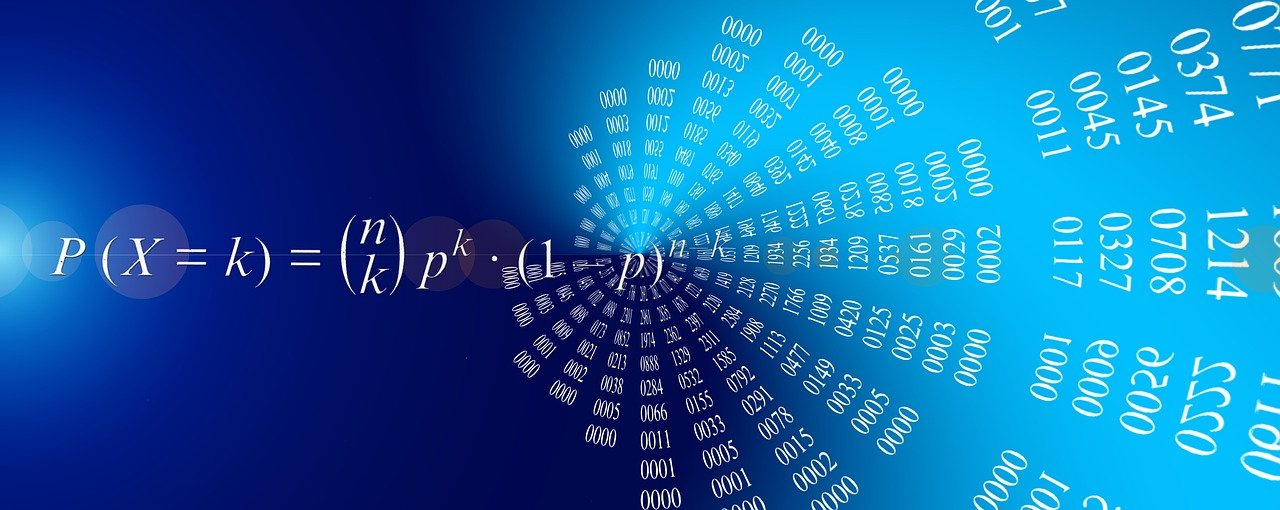
\includegraphics[width=1\textwidth]{imagenes/part2.png}}}

\chapter{Cálculo de probabilidades}

%*************************************************************************
% ATENcION: por cambio ordenación temas, 2 <--> 3, las imagenes de 3.Prob. 
%están en imagenes02 y las imágenes de 2.Estad 2D están en imagenes03.
%*************************************************************************



\begin{tikzpicture}
	\fill [left color=red!50, right color=teal!50] (0,0) rectangle (6.5,.1);
	\fill [left color=teal!50, right color=green!50] (6.5,0) rectangle (11.5,.1);
	\end{tikzpicture}
	
\section{Introducción}

La teoría de la probabilidad es un modelo matemático que se ocupa de analizar los fenómenos aleatorios en contraposición a los fenómenos deterministas (aquellos en los cuales el resultado del experimento que se realiza, atendiendo a determinadas condiciones, produce un resultado único y previsible que se repetirá la cantidad de veces que éste vuelva a hacerse siempre y cuando se respeten las mismas condiciones).

El origen de la probabilidad reside en la necesidad del ser humano de anticiparse a los hechos y de predecir en cierta medida el futuro para lo que  se construyen patrones y conexiones que intentan poder algo de orden en el caos.

El término probabilidad proviene probable, o sea, de aquello que es más posible que ocurra, y se entiende como el mayor o menor grado de posibilidad de que un evento \emph{aleatorio, estocástico o de azar} ocurra.

Estas tres palabras proceden de nuestras tres culturas:

\begin{itemize}
\item \emph{Aleatorio}, deriva del latín ``aleatorius'', es  `lo que no se puede predecir'. 

\item \emph{Estocástico}, del griego ``stochastikós''  y significa `hábil en conjeturar'.

\item \emph{Azar}, del árabe hispánico ``azzahr'' y hacía alusión a una flor, la misma que se pintaba en una taba (hueso utilizado antiguamente para jugar a algo parecido a los dados), de ahí que finalmente la palabra azar se relacionara con la buena o mala `fortuna'.
\end{itemize}

La idea de probabilidad es uno de esos conceptos que cualquier ser humano tiene preaprendido. Todos tenemos conocimiento intuitivo de lo que supone que una cosa sea muy difícil  que ocurra (acertar en la lotería) o de  algo que sea más fácil que ocurra (lanzar una moneda y que salga cara). Otra cosa es la definición matemática. Desde el punto de vista formal, el concepto de probabilidad  se puede abordar desde tres puntos de vista diferentes: \subrayado{$\textbf{Bernouilli, Laplace y Kolmogorov}$}, como veremos en próximas secciones.


La importancia de la probabilidad radica en que, mediante este recurso matemático, es posible ajustar de la manera más exacta posible los imponderables debidos al azar en los más variados campos tanto de la ciencia como de la vida cotidiana.

La teoría de la probabilidad se aplica en áreas variadas del conocimiento, tanto en ciencias (estadística, matemática, física, química, astronomía, meteorología, medicina) como en ciencias sociales (sociología, psicología social, economía).

\section{Sucesos}

\begin{definition}
.	\textbf{Experimento aleatorio, estocástico o de azar} es aquel que, aún repetido en análogas condiciones, tiene un \emph{resultado impredecible}, siempre da resultados diferentes.

Son experimentos aleatorios:

--- Lanzar una moneda al aire para observar si al caer sale cara o cruz.

--- Sacar y observar el resultado al extraer una carta de una baraja.

--- Lanzar un dado para observar la puntuación obtenida.

\end{definition}


\begin{myexampleblock}{Controversia}
\begin{small}
Existe cierta controversia\footnote{Angulo Bustíos, César (2011). `1'. Estadística. Universidad de Piura. ISBN 978-9972-48-137-6.} sobre si los fenómenos aleatorios existen realmente o simplemente surgen del desconocimiento de los factores que desencadenan el mismo o de las leyes físicas que lo rigen. Por ejemplo, si en el lanzamiento de un dado conociéramos exactamente la fuerza, altura al suelo y ángulo del lanzamiento, las dimensiones exactas del dado y las propiedades del suelo, se podría mediante complejos cálculos conocer el resultado final. Es por esto que algunas veces se define un fenómeno aleatorio como aquel en el que pequeños cambios en sus factores producen grandes diferencias en su resultado (teoría del caos).

\vspace{2mm} Esto no quiere decir necesariamente que exista un completo determinismo científico, sino que en ocasiones el azar es consecuencia de la ignorancia de un suceso o de la incapacidad para procesar toda la información que se tiene.

\vspace{2mm} Algunas propuestas realizadas desde la física, como la interpretación de Copenhague de la mecánica cuántica sostienen que a nivel atómico existen los fenómenos aleatorios genuinos.

\vspace{2mm} Recientemente ha aparecido la propuesta de que algunos sistemas físicos, en concreto los sistemas macroscópicos caóticos podrían ser genuinamente no-computables aunque deterministas, eso implica que aun siendo deterministas no es posible calcular con seguridad su evolución futura, mostrando un comportamiento aparentemente aleatorio.\end{small}
\end{myexampleblock}

\begin{definition}
.	\textbf{Espacio muestral} de un experimento aleatorio es `el conjunto de todos los resultados posibles de un experimento aleatorio', se representa por $E$ o $\Omega$.

--- Para el caso del lanzamiento de una moneda, $E=\{C,X\}$, esto es, sale cara o cruz. 

--- Para el resultado de extraer una carta de de una baraja española, $E=\{1oros, 2oros, \cdots 12bastos\}$, es decir, una cualquirera de las cuarenta cartas que componen la baraja \textcolor{gris}{($\{1,2,3,4,5,6,7,10=sota, 11=caballo, 12=rey ;\ oros, \ copas,\ espadas,\ bastos\}$)}.	

--- Para el lanzamiento de una dado, $E=\{1,2,3,4,5,6\}$
\end{definition}


\begin{theorem}
.	\textbf{Tipos de espacios muestrales}:

\begin{itemize}
	\item Espacios muestrales \textbf{Discretos o numerables}
		\begin{itemize}
			\item Espacios muestrales \textbf{finitos}.
			
			Constan de un número finito de elementos, por ejemplo, \emph{`lanzamiento de un dado'}: $\ E=\{1,2,3,4,5,6\}$
			\item Espacios muestrales \textbf{infinitos numerables}.
			
			Constan de un número infinito numerable de elementos, por ejemplo, \emph{`lanzar un dado hasta obtener un cinco'}: $\ E=\mathbb N$
		\end{itemize}
	\item Espacios muestrales \textbf{continuos}, que siempre son infinitos no numerables.	
	
	Constan de un número infinito no numerable de elementos, por ejemplo, \emph{elección al azar de un número del intervalo [0,1]}: $\ E=[0,1]$
\end{itemize}	
\end{theorem}


\begin{destacado}
Seria conveniente dar un vistazo al  apendice \ref{cjtos}  Conjuntos.	
\end{destacado}


\begin{definition}
.	\textbf{Suceso} aleatorio: es cada uno de os subconjuntos del espacio muestral.

--- En el experimento de lanzar un dado, $E=\{1,2,3,4,5,6\}$, son sucesos:

\begin{multicols}{2}
	$A=\{2,4,6\}: \text{ `ha salido par'}$
 
	$B=\{3,6\}: \text{ `es múltiplo de 3'}$

	$C=\{1\}: \text{ `sale el uno'}$

	etc 
\end{multicols}
\end{definition}

\subsection{Tipos de sucesos}

\begin{definition}
.	\textbf{Sucesos elementales:} están formados por un solo elemento del espacio muestral.

\textbf{Sucesos compuestos:} formados por dos o más elementos de espacio muestral (o por ninguno).

\vspace{2mm} \textbf{Suceso seguro:} es es que siempre se verifica, coincide con el espacio muestral $E$.

\textbf{Suceso imposible:} es el que nunca se verifica, se representa por $\emptyset$ (se trata del suceso formado por ningún elemento del espacio muestral, el conjunto vacío -- ver apéndice \ref{cjtos} --)

\vspace{2mm} \emph{Los sucesos son subconjuntos del espacio muestral, incluidos el propio $E$ y el conjunto vacío  $\emptyset$} (subconjuntos impropios).
\end{definition}

\begin{example}
. En el experimento de lanzar un dado, 	$E=\{1,2,3,4,5,6\}$,

\begin{multicols}{2}
\begin{small}
$\{1\}$ es un suceso elemental.

$\{1,2,3,4,5,6\}$ es el suceso seguro.

$\{2,4,6\}$ es un suceso compuesto.	

$\emptyset$ es el suceso imposible. \textcolor{gris}{$(\{-8.73\})$}
\end{small}
\end{multicols}
\end{example}

El conjunto de \emph{todos} los conjuntos de un espacio muestral recibe el nombre de \textbf{espacio de sucesos} y se deisgna por $\mathcal S$

\vspace{2mm} En el experimento del lamzamiento de una moneda:
$E=\{C,X\}$ y $\mathcal S= \left\{  {\emptyset, \{C\}, \{X\};  E} \right\} $ 

\begin{theorem}
. Si en un experimento aleatorio el espacio muestral tiene $n$ elementos, se puede hablar de hasta $2^n$ sucesos en el espacio de sucesos.

\vspace{2mm} Al número de elementos de un conjunto $X$ se le llama cardinal, $card(X)$. Entonces,

$$\text{Si } \ \boldsymbol{ card(E)\ = \ n \ \Rightarrow \ card(\mathcal S)\ = \ 2^n } $$ 
\end{theorem}

\begin{proof}
Como los sucesos no son más que subconjuntos, probar este teorema consiste en probar que para un conjunto de $n$ elementos, el conjunto de sus \emph{partes} (subconjutos) tiene $2^n$ elementos. Puede verse esta demostración en el apéndice \ref{cjtos}.	
\end{proof}

\begin{definition}
.	Dado un suceso cualquiera de un experimento aleatorios, $A\subset E$, se llama \textbf{suceso contrario o complementario} de $A$, que denotaremos por $A',\ \overline{A} \text{ o } A^C$ a aquel suceso que se verifica cuando no lo hace el suceso $A$. 

\vspace{2mm} Evidentemente, $\quad \boldsymbol {(A')'\ =\ A} $

\vspace{2mm} Al lanzar un dado, el suceso contrario a $A=$ \emph{`ha salido 2 o 5'} $=\{2,5\}$, es $A'=\{1,3,4,6\}$. 
\end{definition}

\subsection{Operaciones con sucesos}

\begin{definition}

Dados dos sucesos de un espacio muestral asociado a un experimento aleatorio, $A,\ B \ \subset \ E$, se definen:

\begin{multicols}{2}
	\vspace{4mm} \textbf{Suceso unión, $A\cup B$}, es el suseso que se verifica siempre que lo hagan $A$ o $B$ o ambos.
	
	$$\subrayado{\  \boldsymbol{A\ \cup \ B} \ }$$

	\begin{figure}[H]
			\centering
			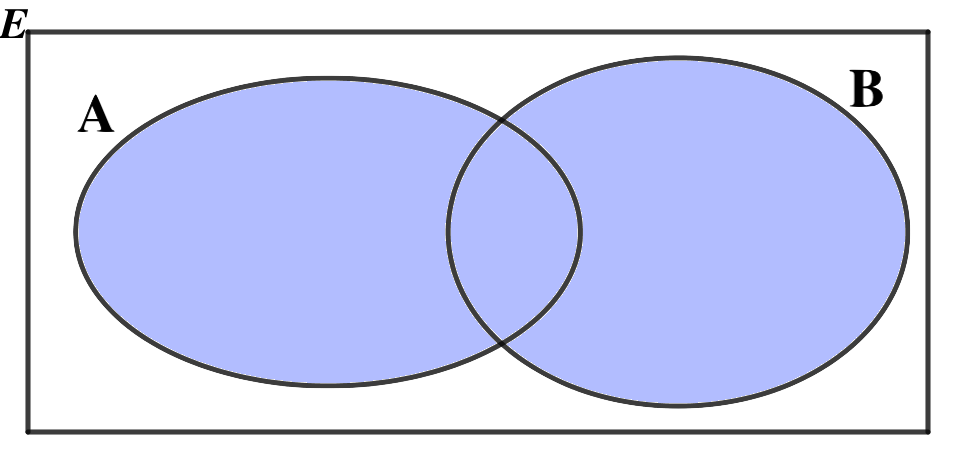
\includegraphics[width=0.5\textwidth]{imagenes/imagenes02/T02IM02.png}
	\end{figure}
\end{multicols}
	
	
\begin{multicols}{2}
	\vspace{4mm} \textbf{Suceso Intersección, $A\cap B$}, es el suseso que se verifica siempre que lo hagan $A$ y $B$ simultáneamente.
	
	$$\subrayado{\  \boldsymbol{A\ \cap \ B} \ }$$

	\begin{figure}[H]
			\centering
			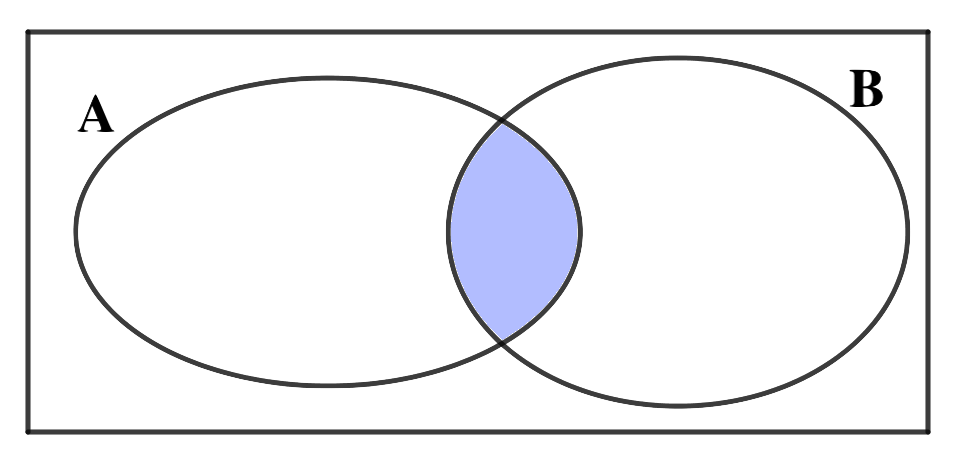
\includegraphics[width=0.5\textwidth]{imagenes/imagenes02/T02IM03.png}
	\end{figure}
\end{multicols}

\begin{multicols}{2}
	\vspace{4mm} \textbf{Suceso Complementario, $A'$}, es el suseso que se verifica siempre que no lo haga $A$.
	
	$$\subrayado{\  \boldsymbol{A'} \ }$$

	\begin{figure}[H]
			\centering
			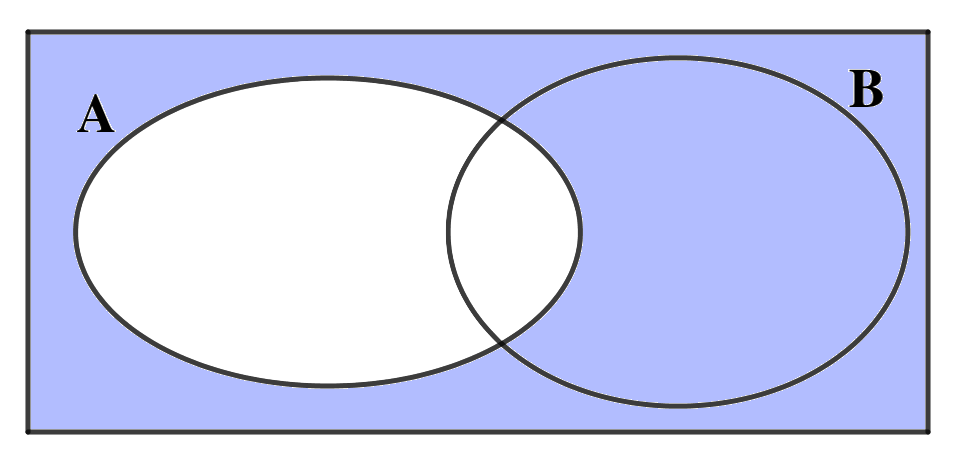
\includegraphics[width=0.5\textwidth]{imagenes/imagenes02/T02IM04.png}
	\end{figure}
\end{multicols}


\begin{multicols}{2}
	\vspace{4mm} \textbf{Suceso diferencia, $A - B$} o $A\ \backslash \ B$, o $A \sim B$, es el suseso que se verifica siempre que lo haga $A$ pero no lo haga $B$.
	
\vspace{-4mm}	$$\subrayado{\  \boldsymbol{A\ - \ B \ = \ A\ \backslash \ B \ = \ A \ \sim \ B} \ }$$

	\begin{figure}[H]
			\centering
			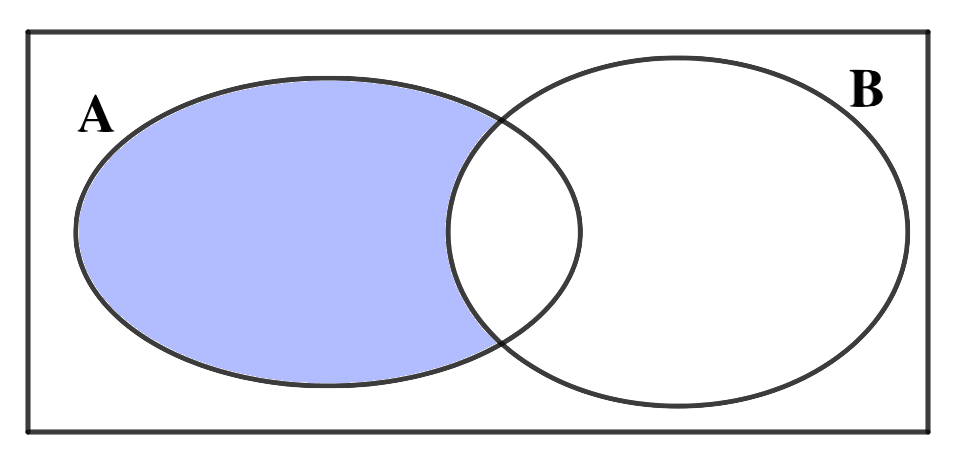
\includegraphics[width=0.5\textwidth]{imagenes/imagenes02/T02IM05.png}
	\end{figure}
\end{multicols}

\end{definition}

\begin{theorem}
.	$$A-B\ = \ A\cap B'$$	\label{dif-comp}
\end{theorem}

\begin{proof}
Presentamos estos diagramas de Ven como prueba. En el de la derecha, $A$ está rayado en vertical y $B'$ en horizontal, por tanto, la intersección es la zona en que se cruzan las líneas.	
	\begin{multicols}{2}
	\begin{figure}[H]
			\centering
			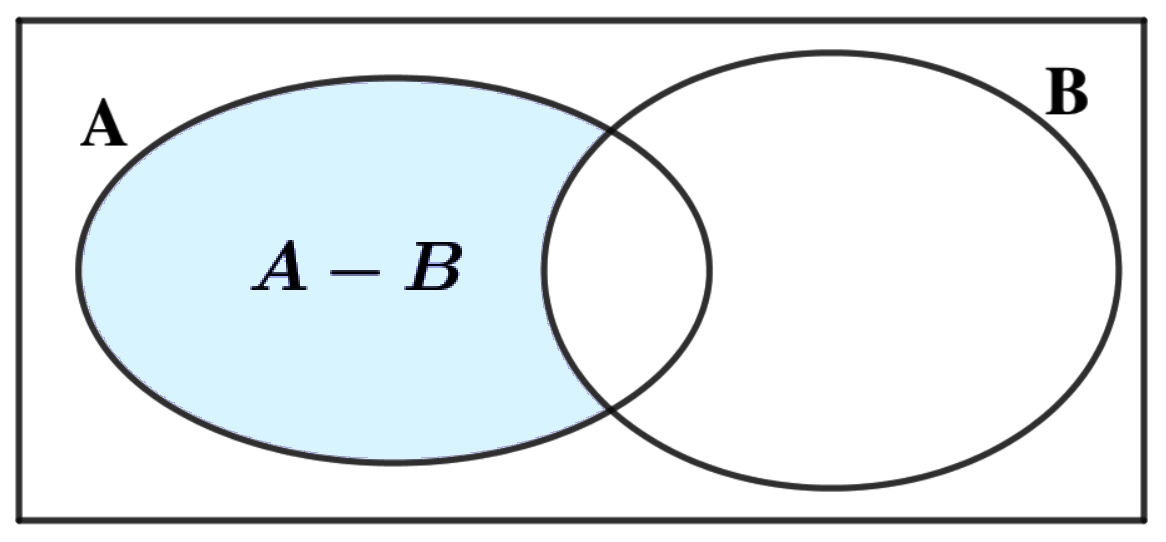
\includegraphics[width=0.5\textwidth]{imagenes/imagenes02/T02IM07.png}
	\end{figure}
	\begin{figure}[H]
			\centering
			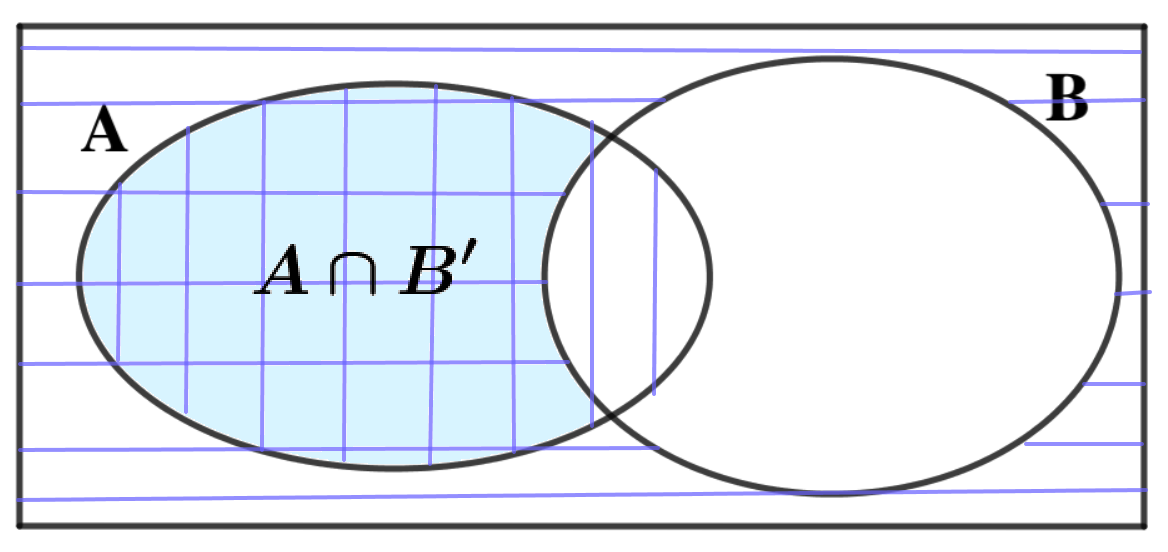
\includegraphics[width=0.5\textwidth]{imagenes/imagenes02/T02IM08.png}
	\end{figure}
	\end{multicols}
\end{proof}

\begin{definition}
.
\begin{multicols}{2}
	Dos sucesos $A \text{ y } B$ son \textbf{incompatibles} si no se verifican nunca simultáneamente, es decir,

$\boldsymbol{ A \text{ y } B  \textbf{ incompatibles si }}$

$\boldsymbol{ A\cap B=\emptyset }$	


	\begin{figure}[H]
			\centering
			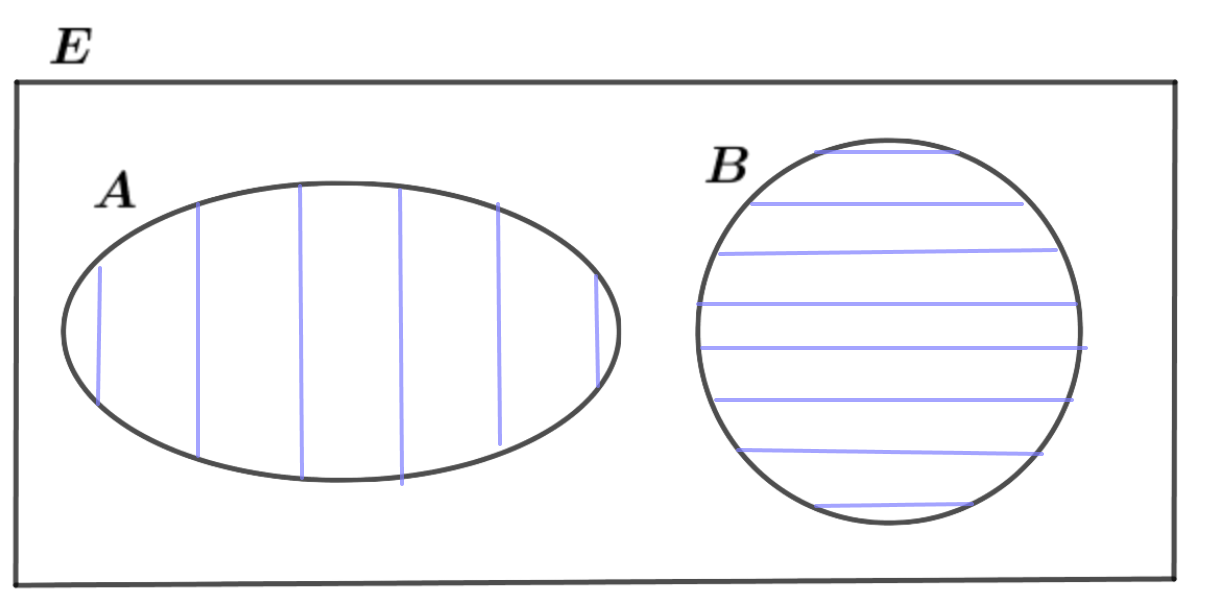
\includegraphics[width=0.5\textwidth]{imagenes/imagenes02/T02IM06.png}
	\end{figure}
\end{multicols}

Evidentemente, $A$ y $A'$ son incompatibles.

Si $A$ y $B$ sí pueden verificarse simultáneamente, $\boldsymbol{A\cap B\neq \emptyset}$, decimos que A y B son \textbf{compatibles}.
\end{definition}


Por ejemplo, los sucesos A=``sale par'' y B=``sale impar'' al lanzar un dado son sucesos incompatibles.

\begin{destacado}
En muchos casos, para obtener el espacio muestral, resulta conveniente dibujar un \emph{\textbf{``diagrama de árbol''}}  (Ver apéndice \ref{combinatoria} Combinatoria), sobre todo en \textbf{experimentos compuestos}, \emph{los que constan de dos o más partes}, como el lanzamiento de dos monedas (o dados) donde, para analizar todos los posibles resultados, consideramos que primero lanzamos la primera moneda y luego la segunda.
\end{destacado}


\begin{theorem}
. Propiedades de las operaciones con sucesos.

Sean $A,\ B, \text{ y } C$ sucesos. $E$ el suceso seguro y $\emptyset$ el seguro imposible, se cumple:

\begin{table}[H]
\centering
\begin{tabular}{l|c|c|}
\cline{2-3}
 & \textbf{Unión $\ \boldsymbol{\cup}$} & \textbf{Intersección $\ \boldsymbol{\cap}$} \\ \hline
\multicolumn{1}{|l|}{\textit{1. Asociativa}} & \begin{tabular}[c]{@{}c@{}}$A \cup (B \cup C)=$\\ $(A \cup B) \cup C$\end{tabular} & \begin{tabular}[c]{@{}c@{}}$A \cap (B \cap C)=$\\ $(A \cap B) \cap C$\end{tabular} \\ \hline
\multicolumn{1}{|l|}{\textit{2. Conmutativa}} & $A \cup B=B \cup A$ & $A \cap B = B \cap A$ \\ \hline
\multicolumn{1}{|l|}{\textit{3. Idempotente}} & $A \cup A =A$ & $A \cap A = A$ \\ \hline
\multicolumn{1}{|l|}{\textit{4. Simplificación}} & $A\cup (A\cap B)=A$ & $A\cap (B \cup A)=A$ \\ \hline
\multicolumn{1}{|l|}{\textit{5. Distributiva}} & \begin{tabular}[c]{@{}c@{}}$A\cup (B\cap C)=$\\ $(A \cup B) \cap (A\cup C)$\end{tabular} & \begin{tabular}[c]{@{}c@{}}$A\cap (B\cup C)=$\\ $(A \cap B) \cup (A\cap C)$\end{tabular} \\ \hline
\multicolumn{1}{|l|}{\textit{6. Neutro}} & $A \cup \emptyset = A$ & $A \cap E=A$ \\ \hline
\multicolumn{1}{|l|}{\textit{7. Absorción}} & $A \cup E=E$ & $A \cap \emptyset = \emptyset$ \\ \hline
\multicolumn{1}{|l|}{\textit{8. Complementario}} & $A \cup A'=E$ & $A \cap A'=\emptyset$ \\ \hline
\multicolumn{1}{|l|}{\textit{9. Leyes de Morgan}} & $(A \cup B)'= A' \cap B'$ & $(A\cap B)'=A' \cup B'$ \\ \hline
\end{tabular}
\end{table}
	
\end{theorem}




\begin{ejemplo}
\begin{ejre}
Encuentra el espacio muestral asociado al experimento aleatorio consistente en lanzar tres monedas al aire. Si se define el suceso A=\emph{`al menos una de las monedas es cara'}, ?`de cuántos sucesos elementales consta el suceso A?	Describe el suceso B=`salen dos caras' 
\end{ejre}
\vspace{4mm} 
% Set the overall layout of the tree
\tikzstyle{level 1}=[level distance=1.5cm, sibling distance=2cm]
\tikzstyle{level 2}=[level distance=1.5cm, sibling distance=1cm]
\tikzstyle{level 3}=[level distance=4.5cm, sibling distance=.5cm]

% Define styles for bags and leafs
\tikzstyle{bag} = [text width=2em, text centered]
\tikzstyle{end} = [circle, minimum width=3pt,fill, inner sep=0pt]

\begin{tikzpicture}[grow=right, sloped]
\node {}
    child {
        node[bag] {$X$}  
            child {
                node {$X$}{}
            		child {
            		node {$X \qquad \textcolor{gris}{XXX} \quad 2\cdot 2 \cdot 2 = 8 \text{ casos}$}
            		}
            		child {
            		node {$C  \qquad \textcolor{gris}{XXC} $}
            		}
            }
            child {
                node {$C$}{}
            		child {
            		node {$X  \qquad \textcolor{gris}{XCC} $}
            		}
            		child {
            		node {$C  \qquad \textcolor{gris}{XCX} $}
            		}
            }
    }
    child {
        node[bag] {$C$}   
            child {
                node {$X$} {}
                	child {
            		node {$X  \qquad \textcolor{gris}{CXX} $}
            		}
            		child {
            		node {$C  \qquad \textcolor{gris}{CXC} $ }
            		}
            }
            child {
                node {$C$} {}
               		child {
            		node {$X  \qquad \textcolor{gris}{CCX} $}
            		}
            		child {
            		node {$C  \qquad \textcolor{gris}{CCC} $}
            		}
            } 
    }
    ;
\end{tikzpicture}

$E=\{CCC,\ CCX,\ CXC,\ CXX,\ XCC,\ XCX,\ XXC,\ XXX  \}$

\textbf{En muchas ocasiones, para determinar un suceso es más sencillo si se piensa en el suceso contrario}: $A'=$ `no sale ninguna cara'=`todas son cruces' $=\{XXX \}$. Entonces, $A=E-A'=\{CCC,\ CCX,\ CXC,\ CXX,\ XCC,\ XCX,\ XXC,  \}$, el suceso A está formado por 7 elementos.

B=`salen dos caras'=`una de las monedas es cruz y las otras dos caras'=$\{XCC,\ CXC,\ CCX\}$, está formado por tres sucesos elementales.
\end{ejemplo}

\begin{ejemplo}
\begin{ejre}
Una bolsa contiene 10 bolas numeradas del 1 al 10. La experiencia aleatoria consiste en extraer una bola y observar su número. Sean A=`obtener número primo' y B=`obtener múltiplo de tres', describe los sucesos $A$, $B$, $A\cap B$, $A\cup B$, $A'$, $B'$, $A-B$, $B\cap A'$, $(A\cap B')'$	

\vspace{4mm} \textbf{En muchas ocasiones, para determinar operaciones con sucesos son muy útiles los diagramas de Venn}


	\begin{figure}[H]
			\centering
			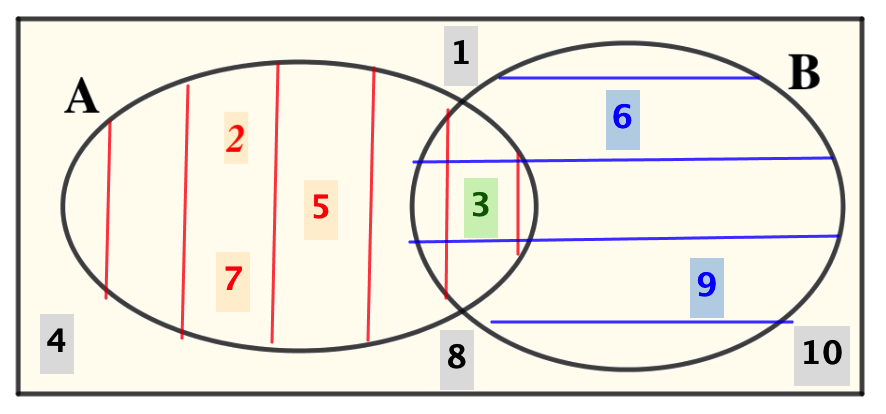
\includegraphics[width=0.6\textwidth]{imagenes/imagenes02/T02IM09.png}
	\end{figure}
	
	
	\begin{scriptsize} En la figura (diagrama de Venn), aparece $A$ dibujado con línea verticales rojas, $B$ con horizontales azules. Donde aparecen las rayas cruzadas es $A\cap B$, cualquier zona rayada es $A\cup B$. La zona rayada sólo verticalmente (rojo)es $A-B$, la rayada sólo horizontalmente (azul) $B-A$.\end{scriptsize}
	\begin{scriptsize} El complementario de $A$, $A'$ será toda la zona del rectángulo excepto la zona rayada con líneas verticales rojas. El complementario de la unión, $(A\cup B)'$, será toda la zona no rayada de ningún modo. Etc.\end{scriptsize}

$A=$`primo'=$\{2,3,5,7\};\qquad B=$` $\dot{3}$ '$=\{3,6,9\}$

$A\cap B=\{3\}; \qquad A\cup B=\{2,5,7,3,6,9\}$

$A'=\{1,4,6,8,9,10\};\qquad B'=\{1,2,4,5,7,8,10\}$

$A-B=\{2,3,5,7\}-\{3,6,9\}=\{2,5,7\}$

$B\cap A'=\{3,6,9\} \cap \{1,4,6,8,9,10\}=\{6,9\}=B-A$

$(A\cap B')' \ \to \ $ calculemos, previamente, $A\cap B'$, que sabemos que coincide con $A-B$ \textcolor{gris}{(Ver teorema \ref{dif-comp})} y tenemos su resultado:
$A \cap B'=A-B=\{2,5,7\} \ \to \ $

$\to \ (A\cap B')'=E-(A\cap B')=\{1,3,4,6,8,9,10\}$

\end{ejre}	
\end{ejemplo}

\begin{ejemplo}
\begin{ejre}
Se extraen dos cartas de una baraja española (sin reinserción)\footnote{\emph{La extracción de varias cartas de una baraja puede realizarse de dos modos distintos, \textbf{con reinserción} (devolviendo cada carta extraída de nuevo al mazo antes de la siguiente extracción) o \textbf{sin reinserción} (cada carta que se extrae no se vuelve a reinsertar en la baraja).}}

Se consideran los sucesos A=`las dos cartas son de copas' y B=` una carta es de copas y la otra es rey'. Calcula $A\cap B$ y $A\cup B$\footnote{Para la resolución de este ejercicio, consideramos las cartas marcadas con los números de 1 al 10, es decir, la sota será en 8, el caballo el 9 y el rey el 10.}
\end{ejre}
\vspace{4mm} 

Los casos en que se pueden extraer dos copas de una baraja son: la primera carta de copas puede ser una cualquiera de las diez que hay en la baraja. Extraída la primera, la segunda puede ser cualquier de las nueve copas que quedan. Total $10\cdot 9=90$ casos. PERO, hemos contado cada caso dos veces, por ejemplo, si la primera es el `siete de copas' y la segunda el `as de copas' o si la primera es el `as' y la segunda el `siete'; hay que divisor por 2, así, los diferentes casos en que se pueden dos copas de una baraja son 90/2=45.

Si recordamos la combinatoria \subrayado{$(\textbf{ver apéndice }$ \ref{combinatoria} $\textbf{ Combinatoria})$ }, tenemos un conjunto de 10 elementos (cartas  que sean copas en la baraja española) de la que vamos a extraer dos, \emph{sin que nos importe el orden y sin poder repetir} (sin reinserción). Tenemos 

$C_{10}^2=\mqty(10\\2)=\dfrac{10!}{(10-2)!\ 2!}=\dfrac {10\cdot 9\cdot \cancel{8!}}{\cancel{8!}\ 2}=45$

Esquemáticamente, si designamos por  $or,\ co,\ es,\ ba$ respectivamente a las cartas de oros, copas espadas y bastos (palos de la baraja) y por $n$ al número de la misma, $n\in \{1,2,3,\cdots, 9, 10\}$, el suceso pedido es:

$A=\{(n\text{-}co;\ m\text{-}co);\ con \ n<m\in \{1,2,3,\cdots, 9, 10\} \}$ \textcolor{gris}{(Al exigir $n<m$ evitamos que influya el orden y que haya repeticiones).}



El suceso B, usando esta misma notación, sería:

$B=\{(n\text{-}co; rey\text{-}or); \ (n\text{-}co; rey\text{-}co);\ (n\text{-}co; rey\text{-}es);\ (n\text{-}co; rey\text{-}ba);\ \ n\in \{1,2,\cdots 9\} \} U \{(rey-co;rey-or);\ (rey-co;rey-es);\ (rey-co;rey-ba)\}$, en total, $ 9+9+9+9+1+1+1=39$ casos.

Las distintas posibilidades de extraer dos cartas, sin reinserción, de una baraja española son, como se ha explicado anteriormente, $\dfrac{40\cdot 39}{2}=\textcolor{gris}{\mqty(40\\2)}=780$ casos posibles. \textcolor{gris}{(1or,2or), (1or,3or), $\cdots$, (caballo bastos,rey bastos)=(9-ba,rey-ba)}

	\begin{figure}[H]
			\centering
			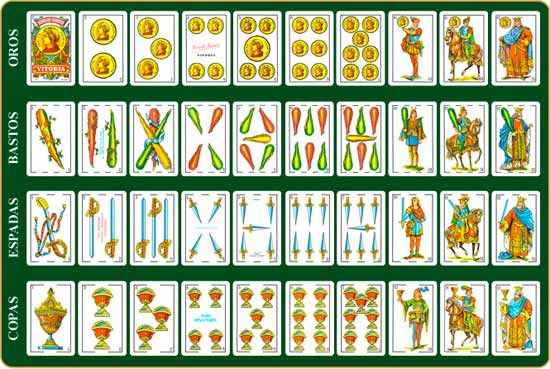
\includegraphics[width=.9\textwidth]{imagenes/imagenes02/T02IM10.png}
	\end{figure}

$\Rightarrow A\cap B=\{(n-co;rey-co);\ n\in \{1,2,\cdots, 9\}\}$, hay 9 casos.

$\Rightarrow A\cup B=  \{(n-co;m-co);\ n<m\ \in\{1,2,\cdots , 9\}\} \ \cup $

$\{(n-co;rey-co);\ n\in \{1,2,\cdots, 9\}\} \  \cup \ $

$\{(n-co;rey-or); (n-co;rey-es); (n-co;rey-ba);\ n\in \{1,\cdots, 9\}\} \ \cup \ $

$\{(rey-or;rey-co);(rey-es;rey-co);(rey-ba;rey-co) \}$

\begin{scriptsize}Es decir, $A\cup B$ está formado por cualquier `pareja de cartas donde una de ellas ha de ser de copas y la otra ha de ser o bien copas o bien un rey'.\end{scriptsize}
\begin{figure}[H]
			\centering
			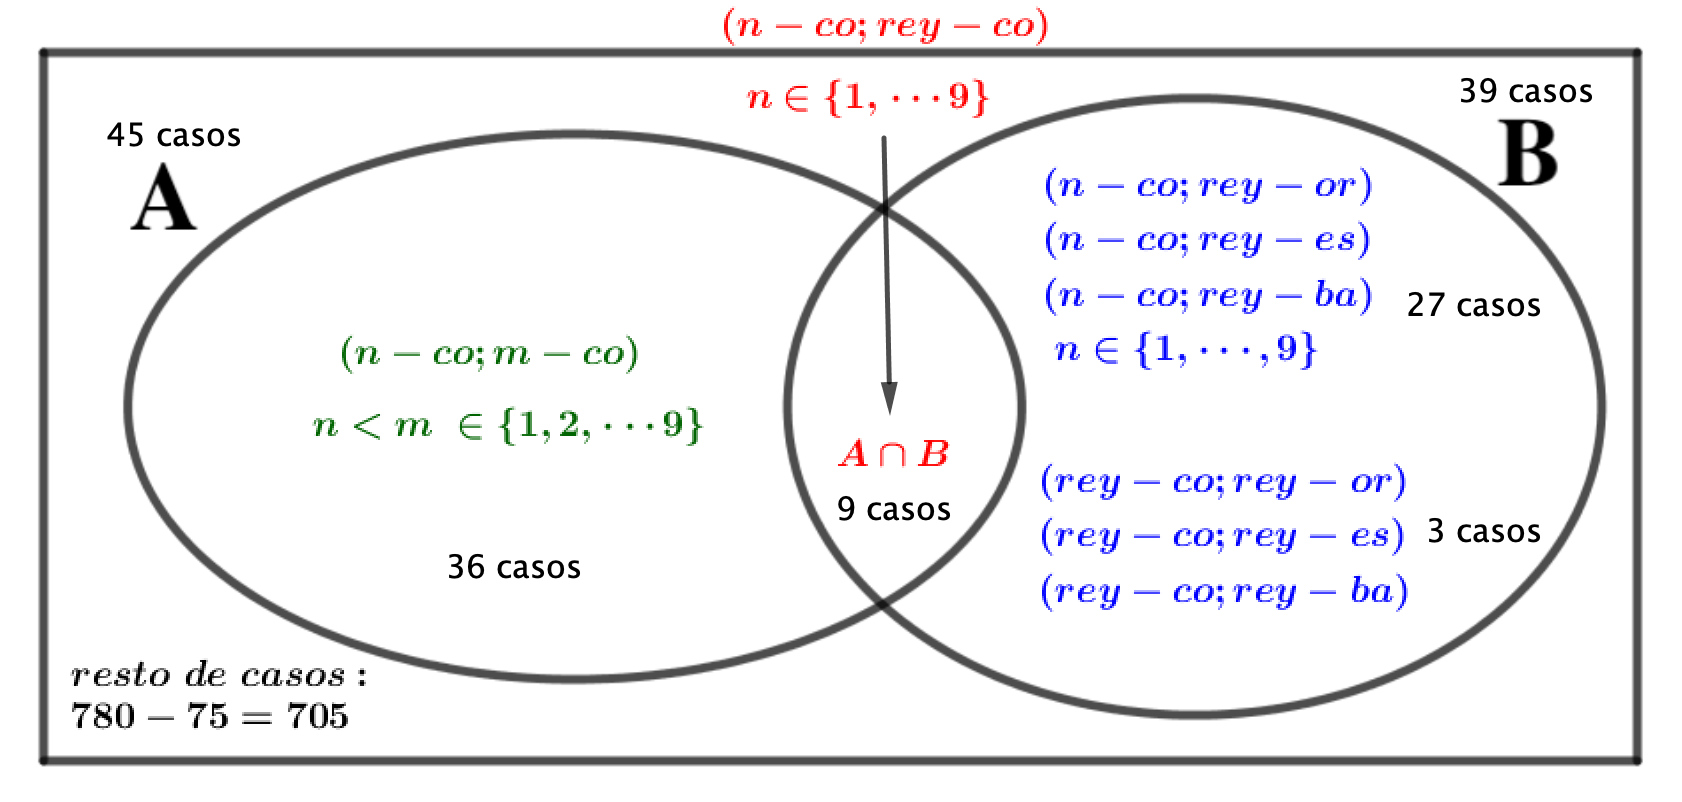
\includegraphics[width=1\textwidth]{imagenes/imagenes02/T02IM11.png}
	\end{figure}
\end{ejemplo}




\section{Probabilidad}

	\begin{figure}[H]
			\centering
			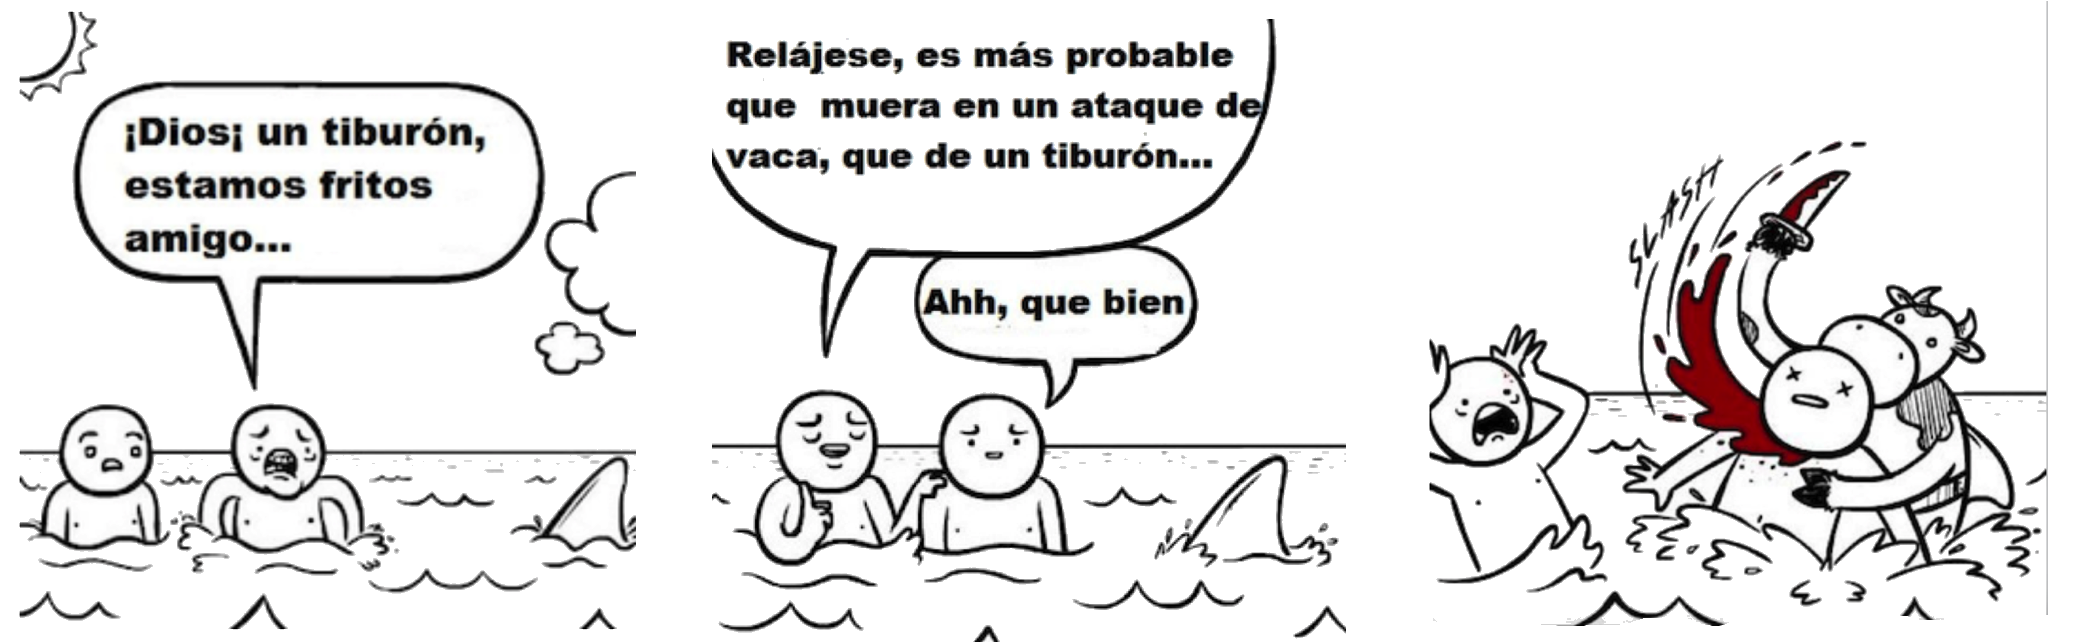
\includegraphics[width=1\textwidth]{imagenes/imagenes02/T02IM01.png}
	\end{figure}

\begin{myexampleblock}{Los inicios de la teoría de la probabilidad.}
\begin{small}La teoría matemática de la probabilidad tuvo como uno de sus primeros puntos de partida el intentar resolver un problema particular concerniente a una apuesta de juego de dados entre dos personas. El problema al que nos referimos involucraba una gran cantidad de dinero y puede plantearse de la siguiente forma:\footnote{Esto cure en la sociedad francesa de 1650, donde el juego era un entretenimiento muy corriente y no demasiado sujeto a restricciones legales. Los juegos eran numerosos y cada vez más complicados, y se apostaban grandes cantidades de dinero.} 

\vspace{2mm}\textit{\textsf{Dos jugadores escogen cada uno de ellos un numero del 1 al 6, distinto uno del otro, y apuestan 32 doblones de oro a que el número escogido por uno de ellos aparece en tres ocasiones antes que el número del contrario al lanzar sucesivamente un dado. Suponga que el numero de uno de los jugadores ha aparecido dos veces y el numero del otro una sola vez. ¿Cómo debe dividirse el total de la apuesta si el juego se suspende?}}

\vspace{2mm}Este problema, que data de la Edad Media, si no antes, es el conocido como ``el problema de la partida interrumpida’’ y fue propuesto por Antoine Gombaud, Caballero de Méré (1607-1684), escritor francés y matemático aficionado a Blaise Pascal (1623-1662) quien lo consultó con Pierre de Fermat (1601- 1665) e iniciarón un intercambio de cartas a propósito del problema. Esto sucede en el año 1654. Con ello se inician algunos esfuerzos por dar solución a éste y otros problemas similares que se plantean.  Con el paso del tiempo se sientan las bases y las experiencias necesarias para la búsqueda de una teoría matemática que sintetice los conceptos y los métodos de solución de los muchos problemas particulares resueltos a lo largo de varios años. 

	\begin{figure}[H]
			\centering
			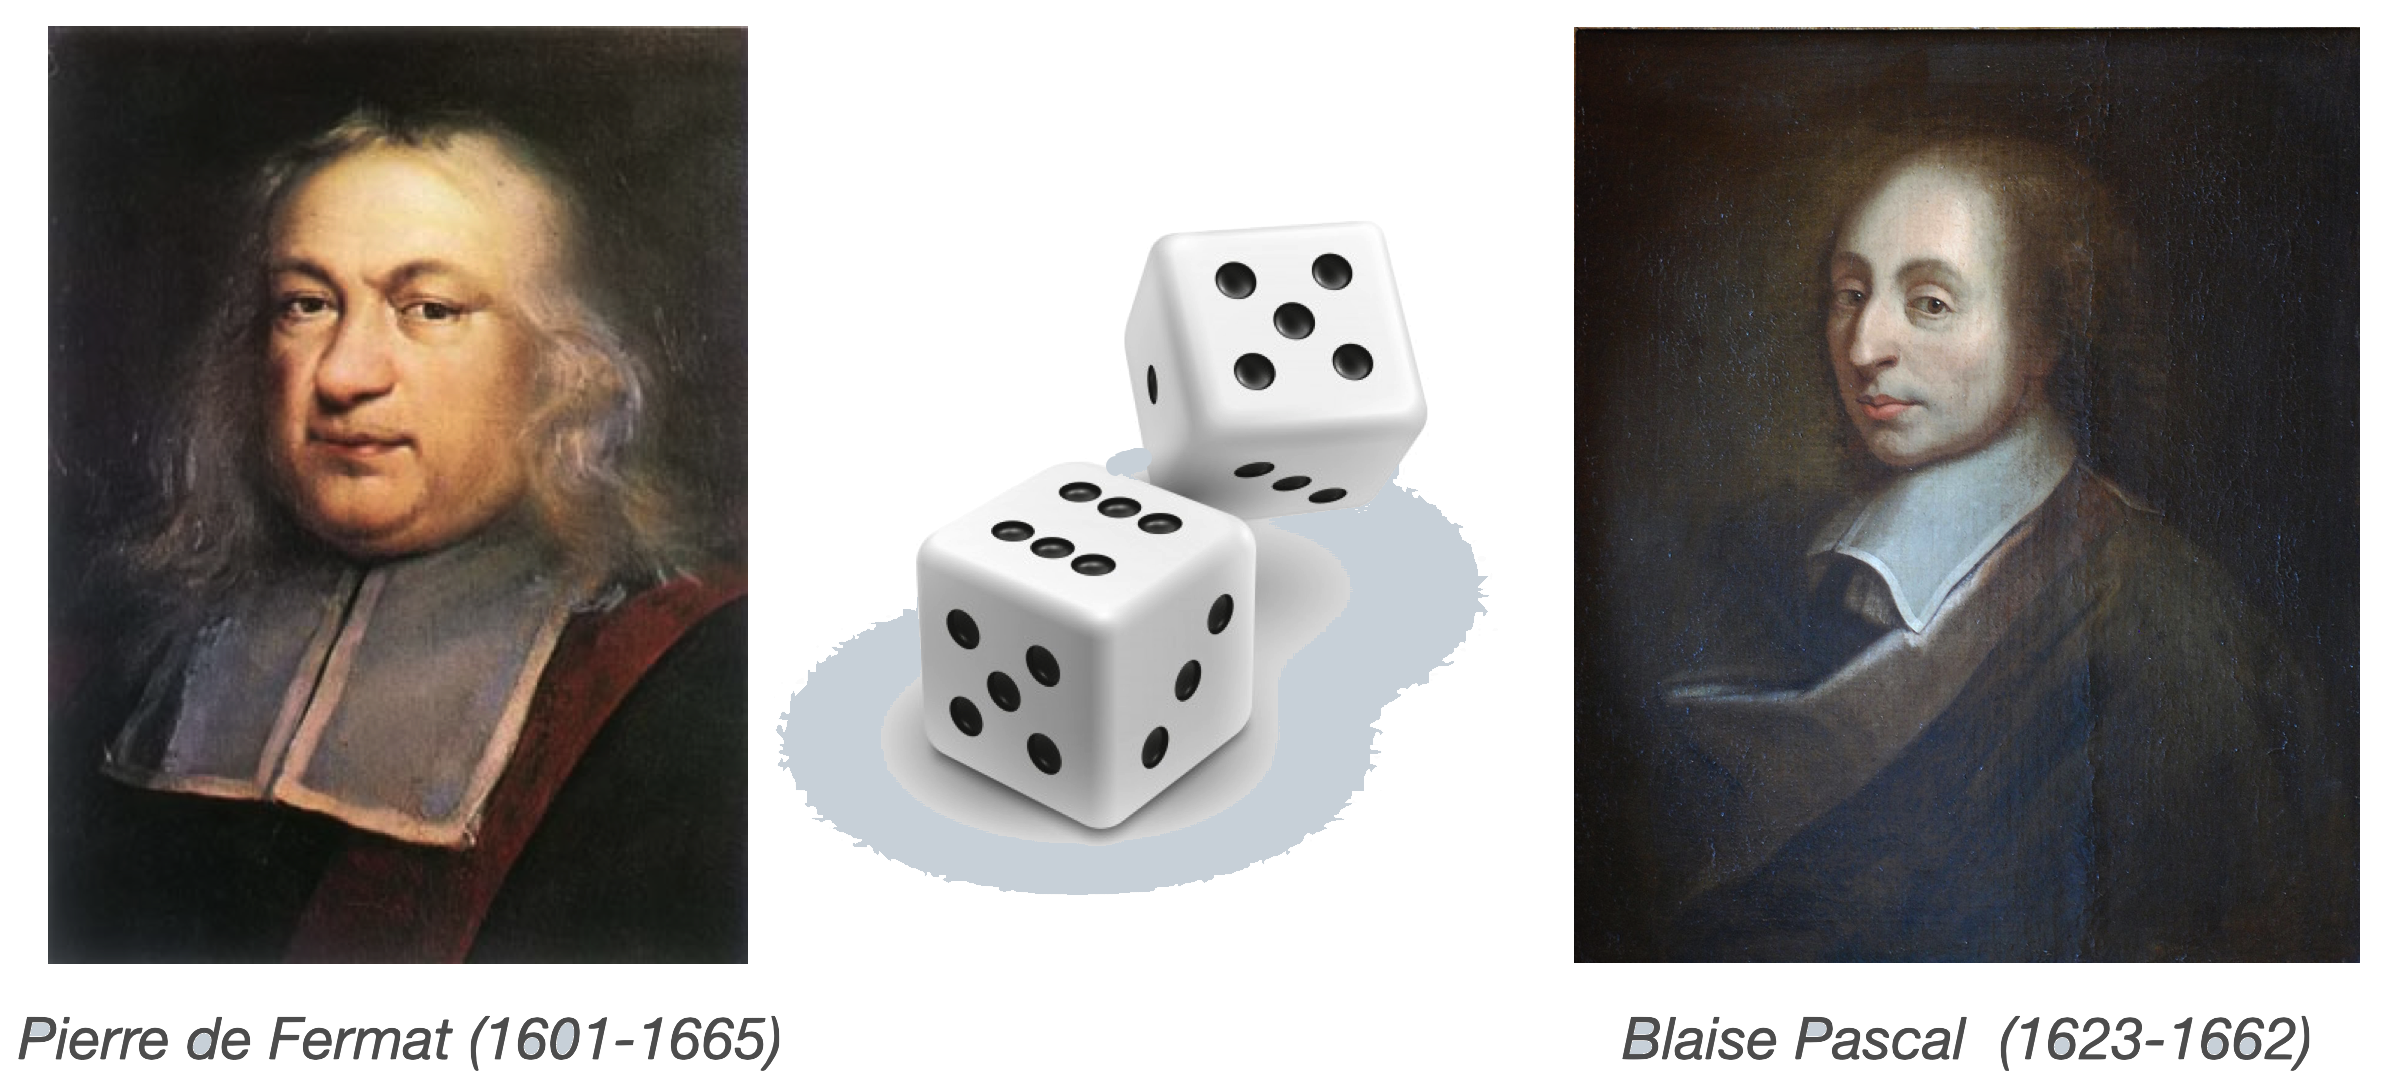
\includegraphics[width=.8\textwidth]{imagenes/imagenes02/T02IM12.png}
	\end{figure}


En el segundo congreso internacional de matemáticas, celebrado en la ciudad de Paris en 1900, el matemático David Hilbert (1862-1943) plantea 23 problemas matemáticos de importancia. Uno de estos problemas es el de encontrar axiomas o postulados a partir de los cuales se pueda construir una teoría matemática de la probabilidad. Aproximadamente treinta años después, en 1933, el matemático ruso A. N. Kolmogorov (1903-1987) propone ciertos axiomas que a la postre resultaron adecuados para la construcción de la teoría de la probabilidad.\end{small}
\end{myexampleblock}

\begin{definition}
.	\textbf{Frecuencia absoluta} de un suceso $A$, $N_A$, es el número de veces que se verifica $A$ cuando se realiza el experimento $N$ veces.

\vspace{2mm} \textbf{Frecuencia relativa} de un suceso es el cociente entre su frecuencia absoluta y el número $N$ de veces que se realiza el experimento, $N_A/N$.
	
\vspace{2mm} \textbf{Ley de los grandes números}: En un experimento aleatorio, al realizar un gran número de pruebas, $N$, la frecuencia relativa de un suceso $A$ tiende a estabilizarse alrededor de un número fijo, $\boldsymbol{p(A)}$, que se llama \textbf{probabilidad} de $A$:

$$\boldsymbol{p(A)\ = \  \mathrm{lim}_{N\to \infty}{\dfrac {N_A}{N}}} $$ 

Esta el la \textbf{\emph{definición frecuencial o ``a posteriori''}} de la probabilidad. Para asignar probabilidades a sucesos se recurre a la experimentación. 

Jacob $\subrayado{\textbf{Bernoulli}}$, 1689, definió la probabilidad usando la ley de los grandes números de Chebishev.
\end{definition}

	
\begin{figure}[H]
			\centering
			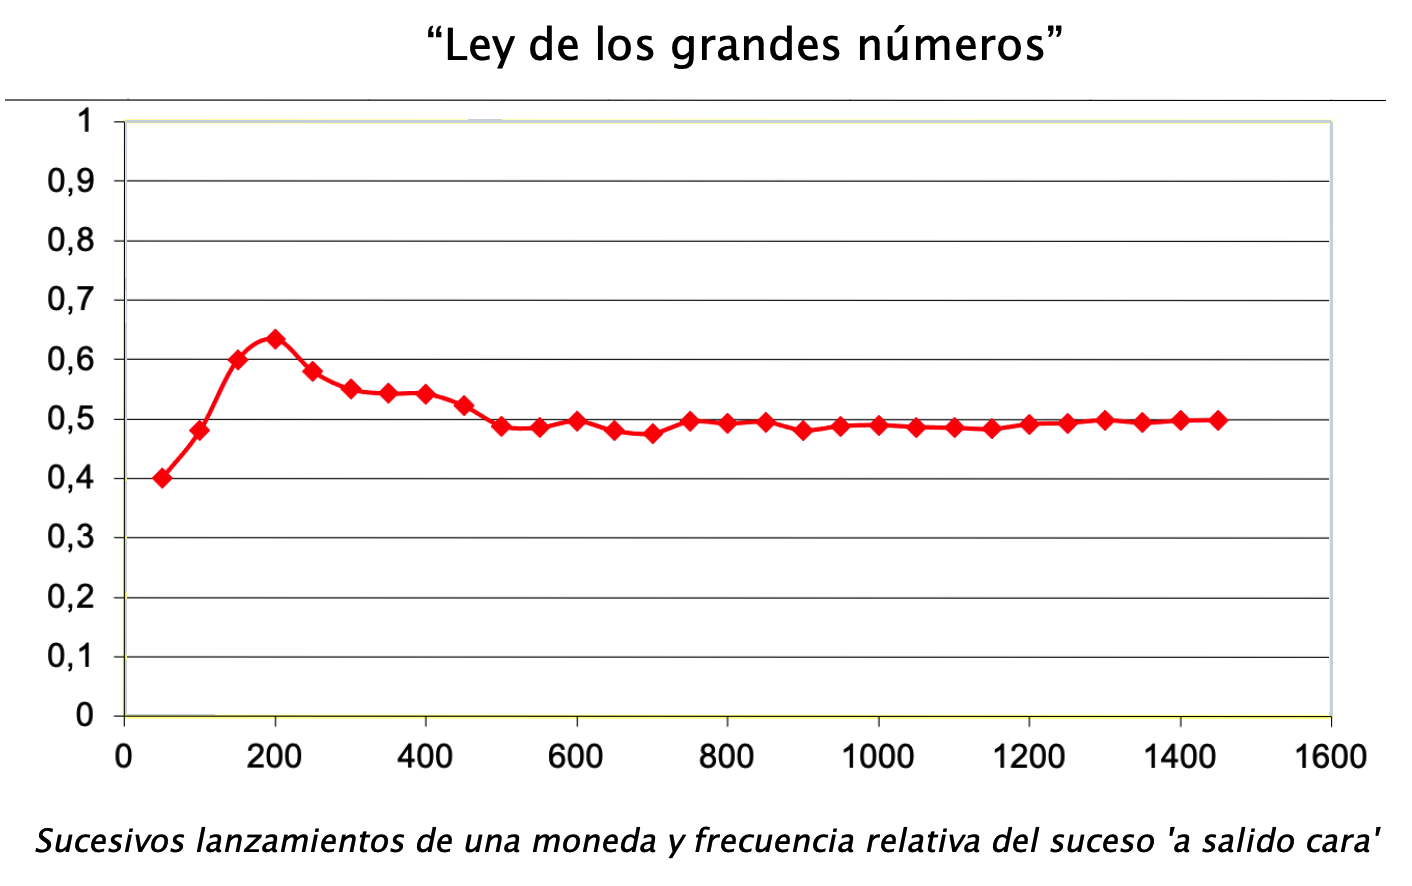
\includegraphics[width=.75\textwidth]{imagenes/imagenes02/T02IM13.png}
			\caption*{Ley de los grandes números}
	\end{figure}	
	
Que la frecuencia se va estabilizando cuando aumenta el número de experiencias es una \emph{verdad empírica}, no demostrable pero sí reiteradamente comprobable. Su enunciado es el \emph{principio básico del azar}, \emph{la ley de los grandes números}.	 
Aunque al principio parezca haber grandes fluctuaciones en la frecuencia relativa, a medida que aumente el número de experimentos éstas se van suavizando y la frecuencia relativa tiende a un número fijo, la probabilidad.
	
\begin{example}
	
Probabilidad de que al lanzar una chincheta sobre la mesa quede con la punta hacia arriba o apoyada en la mesa.

\vspace{2mm} A priori, no lo sabremos, tenemos que recurrir a la experimentación. 

\vspace{2mm} Si dejemos caer 100 chinchetas, y 23 de ellas caen con la punta hacia arriba, estimaremos la probabilidad de este suceso en 0.23. Si dejamos caer 1.000 y obtenemos 307 hacia arriba estimaremos su probabilidad en 0.307, siendo estimación es más segura que la anterior. Y, así sucesivamente, vamos adquiriendo seguridad sobre el valor que asignamos a la probabilidad de ese suceso a medida que aumentemos el número de experimentos realizados. Del mismo modo deberíamos proceder si tuviéramos la sospecha de que, por ejemplo un dado o una moneda están trucados.

	\begin{figure}[H]
			\centering
			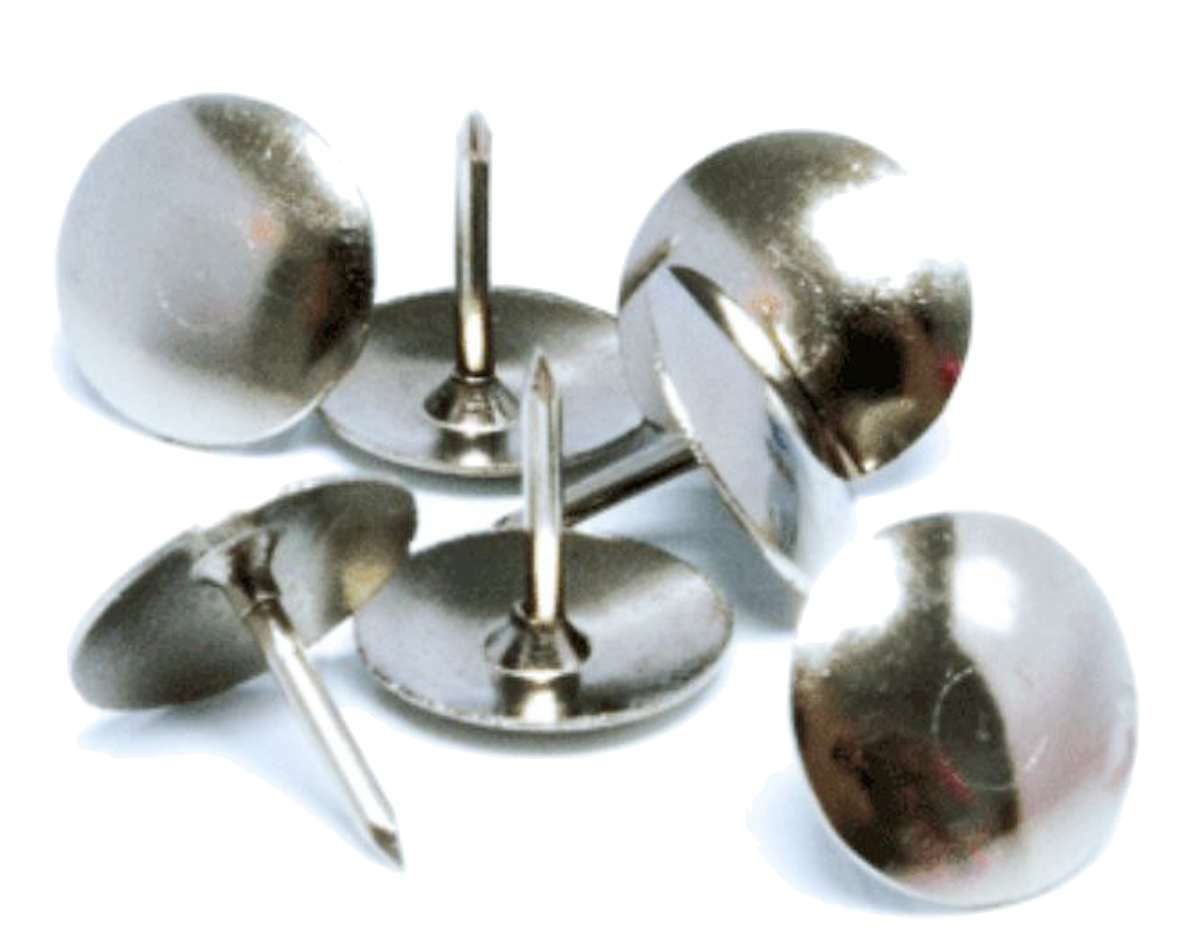
\includegraphics[width=.25\textwidth]{imagenes/imagenes02/T02IM14.png}
	\end{figure} 	
\end{example}	
	
	Esta definición de probabilidad tiene un inconveniente: es necesario realizar un gran número de pruebas para asignar como probabilidades el valor al que se aproximan las frecuencias relativas del suceso en estudio y además, siempre obtenemos un valor aproximado, en lugar del valor exacto de la probabilidad. Es la \emph{asignación de probabilidad $\subrayado{\textbf{``a porteriori''}}$}. En muchas ocasiones no hay otra manera de hacerlo (horas de duración de una batería, nivel de riesgo en una operación, etc).
	
\begin{definition}
. \textbf{Definición clásica de probabilidad. Regla de $\subrayado{\textbf{Laplace}}$}

\vspace{2mm} Pierre Simon Laplace (1749-1827) formula la primera definición que se conoce de probabilidad: \emph{\textbf{``La probabilidad de un suceso $A$, que representaremos por $p(A)$, es el cociente entre el número de casos favorables a dicho suceso y el número de casos posibles’’}}.

$$\boldsymbol{ p(A)\ =\ \dfrac{\textbf{número de casos favorables}}{\textbf{número de casos posibles}} }\textcolor{gris}{\left( = \dfrac{\textbf{ favorables}}{\textbf{ posibles}} \right)}$$

Para aplicar esta definición es necesario que que \emph{los sucesos elementales del espacio muestral han de ser igualmente probables (\textbf{equiprobables})}. 

\vspace{2mm} Son casos favorables los elementos que componen el suceso $A$, y los casos posibles todos los resultados del experimento, es decir, todo el espacio muestral. 

\vspace{2mm} Así, si una experiencia aleatoria consta de $n$ sucesos elementales y es razonable suponer que ninguno de ellos tiene más probabilidad de salir que los demás (equiproblables), la probabilidad de cada uno de ellos es $1/n$.  Para un suceso que conste de $k$ sucesos elementales, su probabilidad será $k/n$. 	
\end{definition}

Esta definición de probabilidad, muchas veces trivial, es en ocasiones muy complicada (determinar si los sucesos son o no equiprobables).  Es la \emph{asignación de probabilidades $\subrayado{\textbf{``a priori’’}}$.}

\begin{example}
.	Calcular la probabilidad de obtener suma $7$ al lanzar dos dados.

\vspace{2mm} El espacio muestral de lanzar dos dados y sumar las puntuaciones obtenidas es $E=\{ 2,3,4,\cdots, 12 \}$, pero, !`CUIDADO!, \underline{todos los sucesos no son equiprobables}. Por ejemplo, obtener suma $6$ se puede hacer con dos `tres'	, pero también con un `cuatro' y un `dos' (0 un 2 y un 4) o un `cinco' y un `uno'; en cambio, suma $12$ solo se obtiene si sales dos `seis'. Para solucionar este aparente problema, consideremos dos dados distintos, observemos los $36$ resultados posibles (por cada uno de los resultados del primer dado, hay $6$ del segundo) y sumemos las puntuaciones obtenidas.

\begin{multicols}{2}
% Please add the following required packages to your document preamble:
% \usepackage[table,xcdraw]{xcolor}
% If you use beamer only pass "xcolor=table" option, i.e. \documentclass[xcolor=table]{beamer}
\begin{table}[H]
\small
\centering
\begin{tabular}{c|c|c|c|c|c|c|}
 & {\color[HTML]{FE0000} \textbf{1}} & {\color[HTML]{FE0000} \textbf{2}} & {\color[HTML]{FE0000} \textbf{3}} & {\color[HTML]{FE0000} \textbf{4}} & {\color[HTML]{FE0000} \textbf{5}} & {\color[HTML]{FE0000} \textbf{6}} \\ \hline
{\color[HTML]{3531FF} \textbf{1}} & 2 & 3 & 4 & 5 & 6 & \underline{7} \\ \hline
{\color[HTML]{3531FF} \textbf{2}} & 3 & 4 & 5 & 6 & \underline{7} & 8 \\ \hline
{\color[HTML]{3531FF} \textbf{3}} & 4 & 5 & 6 & \underline{7} & 8 & 9 \\ \hline
{\color[HTML]{3531FF} \textbf{4}} & 5 & 6 & \underline{7} & 8 & 9 & 10 \\ \hline
{\color[HTML]{3531FF} \textbf{5}} & 6 & \underline{7} & 8 & 9 & 10 & 11 \\ \hline
{\color[HTML]{3531FF} \textbf{6}} & \underline{7} & 8 & 9 & 10 & 11 & 12 \\ \cline{2-7} 
\end{tabular}
\end{table}
	\begin{figure}[H]
			\centering
			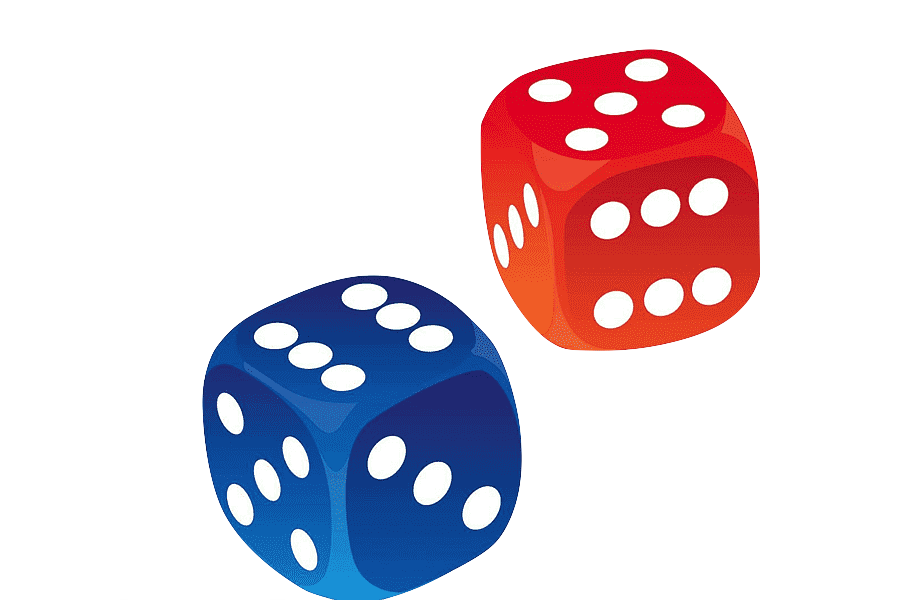
\includegraphics[width=.4\textwidth]{imagenes/imagenes02/T02IM15.png}
	\end{figure}
\end{multicols}
Ahora sí, vemos que de los 36 sucesos posibles, solo en \underline{6 ocasiones} la suma es siete, por lo que p(suma 7)=6/36 (es la suma más probable).	
\end{example}

\begin{myalertblock} {Probabilidades a priori y a posteriori} 

Son  \textbf{probabilidades a priori} aquellas que se pueden determinar de antemano, sin realizar ningún tipo de comprobación experimental, \textbf{en base a consideraciones teóricas}. Un ejemplo puede ser el de la probabilidad de obtener un cinco en el lanzamiento de un dado perfecto. 

\vspace{2mm} Son \textbf{probabilidades a posteriori} las que se determinan con posterioridad a la experimentación, \textbf{a través de la experiencia}. Es necesario estimar la probabilidad estudiando el valor límite al que se acercan las frecuencias relativas al realizar un gran número de pruebas en análogas condiciones. \textcolor{gris}{Es importante tener en cuenta, que las frecuencias relativas que se obtienen de un número reducido de pruebas no puede servir para realizar una estimación fiable de la probabilidad de un determinado suceso, es necesario un elevado número de pruebas, precisamente la garantía de que la definición de probabilidad a posteriori sea buena la da la Ley de los grandes números, $N\to \infty$.}
\end{myalertblock}

\begin{definition}
.	\textbf{Definición Axiomática\footnote{Un axioma es un principio o afirmación matemática que se acepta sin demostración. Para que un conjunto de axiomas sea válido, es necesario que a partir de ellos no se llegue a afirmaciones contradictorias.} de probabilidad.} Andrei Nicolaievich $\subrayado{\textbf{Kolmogorov}}$ (1903-1987).

\textbf{Axiomas:}
\begin{enumerate}[{A}1. ]
\item La probabilidad de un suceso es un número positivo	 o nulo: $\ \boldsymbol{p(A)\ge 0}$
\item La probabilidad del suceso seguro es uno: $\ \boldsymbol{p(E)=1}$

Es decir, $\ \subrayado{ \ \boxed{ \  \boldsymbol{0\le p(A) \le 1}  \ } \ }$
\item Si $A$ y $B$ son dos sucesos  \emph{incompatibles} de un experimento aleatorio ($A\cap B=\emptyset$), $\ \boldsymbol{ p(A\cup B)=p(A)+p(B)}$
\end{enumerate}

\textbf{Propiedades:}

\begin{enumerate}[P1. ]
\item Para sucesos complementarios\footnote{En ocasiones, es más sencillo calcular la probabilidad del suceso contrario al que nos piden. En estos casos, esta propiedad resulta de una relevante utilidad.}, $\ \subrayado{ \ \boxed{ \  \boldsymbol{p(A')=1-p(A)} \ } \ }$
\item La probabilidad del suceso imposible es cero: $\ \boldsymbol{p(\emptyset)=0}$
\item Si $A\subset B \to p(A) \le p(B)$
\item En general, para sucesos compatibles, 

$\subrayado{ \  \boxed{ \  \boldsymbol{p(A\cup B)=p(A)+ p(B)-p(A\cap B)} \ } \ }$
\end{enumerate}	
\end{definition}

\textcolor{gris}{$$p(A\cup P \cup C)=p(A)+p(B)+p(C)-p(A\cap B)-p(A\cap C)-p(B\cap C)+p(A\cap B \cap C)$$}

--- Los axiomas establecen que la probabilidad sea una \emph{``medida’’} en matemáticas. 

--- El segundo axioma fija la cantidad total de probabilidad. Pero podría ser cualquier número positivo,  el tomar $p(E) = 1$ es por similitud con las frecuencias relativas y significa que la ``cantidad de probabilidad’’ se dará en ``tantos por uno``. En ocasiones, las probabilidades se dan en \% (lo cual equivale a tomar $p(E)=100$). 

\begin{example}
.	Hallar la probabilidad de que al lanzar tres monedas se obtenga al menos una cara.

\vspace{4mm} Este es un caso en que es mucho más fácil calcular la probabilidad del suceso contrario	. (Propiedad P1).

\vspace{2mm} Sea A=`obtener al menos una cara en tres lanzamientos de una moneda'. Su suceso contrario será $A'$=`salen tres cruces.'

\vspace{2mm} Suponiendo monedas no cargadas y usando la \emph{ley de Laplace}, $P(A')=1/8$, ya que solo en una ocasión de las ocho posibles se obtienen tres cruces, XXX (primera moneda C,X; independientemente, la segunda puede ser C,X; lo mismo para el tercer lanzamiento, C,X).

\vspace{2mm} Luego, $\ p(A)=1-1/8=7/8$. En el siguiente diagrama de árbol pueden contabilizarse estos casos.

	
\textcolor{gris}{\rule{50mm}{0.1mm}}

\begin{footnotesize}
\textcolor{gris}{Distintos resultados en el lanzamiento de una monedas tres veces.}

% Set the overall layout of the tree
\tikzstyle{level 1}=[level distance=1.5cm, sibling distance=2cm]
\tikzstyle{level 2}=[level distance=1.5cm, sibling distance=1cm]
\tikzstyle{level 3}=[level distance=3cm, sibling distance=.5cm]

% Define styles for bags and leafs
\tikzstyle{bag} = [text width=2em, text centered]
\tikzstyle{end} = [circle, minimum width=3pt,fill, inner sep=0pt]
\begin{center}
\begin{tikzpicture}[grow=right, sloped]
\node {}
    child {
        node[bag] {$X$}  
            child {
                node {$X$}{}
            		child {
            		node {$X \qquad \textcolor{gris}{XXX}$}
            		}
            		child {
            		node {$C  \qquad \textcolor{gris}{XXC} $}
            		}
            }
            child {
                node {$C$}{}
            		child {
            		node {$X  \qquad \textcolor{gris}{XCC} $}
            		}
            		child {
            		node {$C  \qquad \textcolor{gris}{XCX} $}
            		}
            }
    }
    child {
        node[bag] {$C$}   
            child {
                node {$X$} {}
                	child {
            		node {$X  \qquad \textcolor{gris}{CXC} $}
            		}
            		child {
            		node {$C  \qquad \textcolor{gris}{CXX} $ }
            		}
            }
            child {
                node {$C$} {}
               		child {
            		node {$X  \qquad \textcolor{gris}{CCX} $}
            		}
            		child {
            		node {$C  \qquad \textcolor{gris}{CCC} $}
            		}
            } 
    }
    ;
\end{tikzpicture}
\end{center}		
\end{footnotesize}	
\end{example}	
	
\begin{example}
.	Al lanzar un dado de Laplace (sucesos elementales equiprobables; dado equilibrado, no lastrado), se consideran los sucesos A=`sale un número impar' y B='sale múltiplo de 3'. Calcular $p(A\cap B) \text{ y } p(A\cup B)$

\vspace{4mm} $A=\{1,3,5\};\ B=\{3,6\} \to A\cap B=\{3\};\ A\cup B=\{1,3,5,6\}$

\vspace{2mm} --- Usando la ley de Laplace, 	$\textcolor{gris}{\left(  \dfrac{\textbf{ favorables}}{\textbf{ posibles}} \right)}$, tenemos:

\vspace{2mm}$\Rightarrow p(A\cap B)= 1/6;\quad p(A\cup B)=4/6$

\vspace{2mm} --- Si usamos pa propiedad P5 de la axiomática de Kolmogorov,

\vspace{2mm}$\Rightarrow p(A\cup B)=p(A)+ p(B)-p(A\cap B)=3/6+2/6-1/6=4/6$
	
\vspace{2mm} --- Simplemente, al observar la figura (diagrama de Venn)

\vspace{2mm} $\Rightarrow p(A\cup B)=4/6$

\begin{figure}[H]
			\centering
			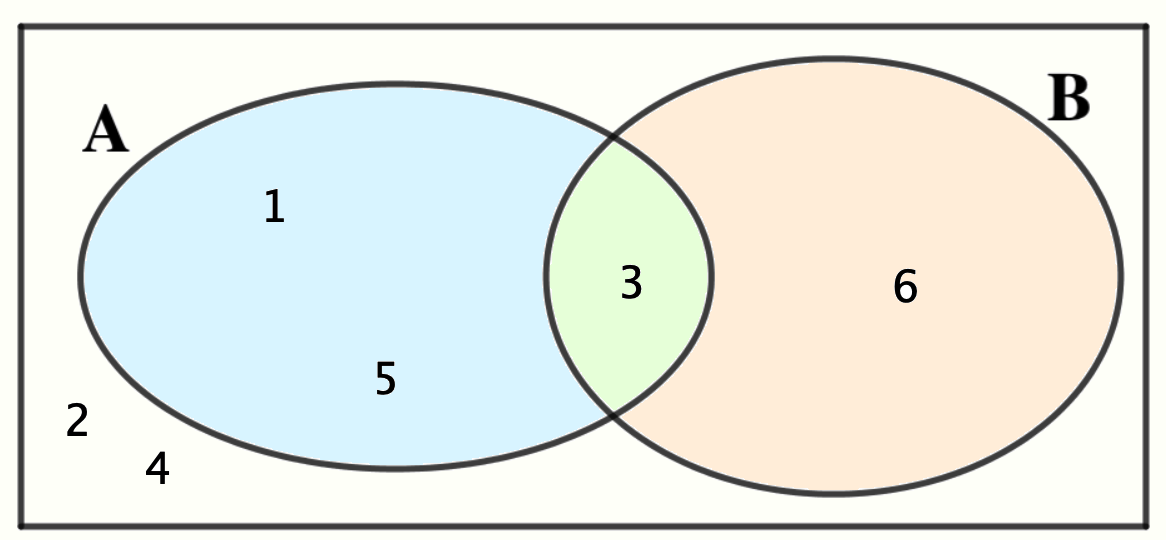
\includegraphics[width=.5\textwidth]{imagenes/imagenes02/T02IM16.png}
	\end{figure}
\end{example}

\begin{ejemplo}
\begin{ejre}
	Supóngase un determinado grupo de personas de entre las que se elige una al azar y en que se consideran los los siguientes sucesos: A='la persona elegida lleva gafas', B=`la persona elegida tiene los ojos marrones'. Se sabe, que en este grupo se dan las siguientes probabilidades: $p(A)=0.4; \ p(B)=0.7; p(A\cap B)=0.23$.
	
	Calcula la probabilidad de que una persona elegida al azar,
	
$a)\ \ $ No lleve gafas.

$b)\ \ $ Use gafas o tenga los ojos marrones.

$c)\ \ $ Lleve gafas pero no tenga los ojos marrones.	
\end{ejre}	

\vspace{4mm} Un \textbf{\emph{diagrama de Venn}} nos ayudará a resolver el problema.

\begin{figure}[H]
			\centering
			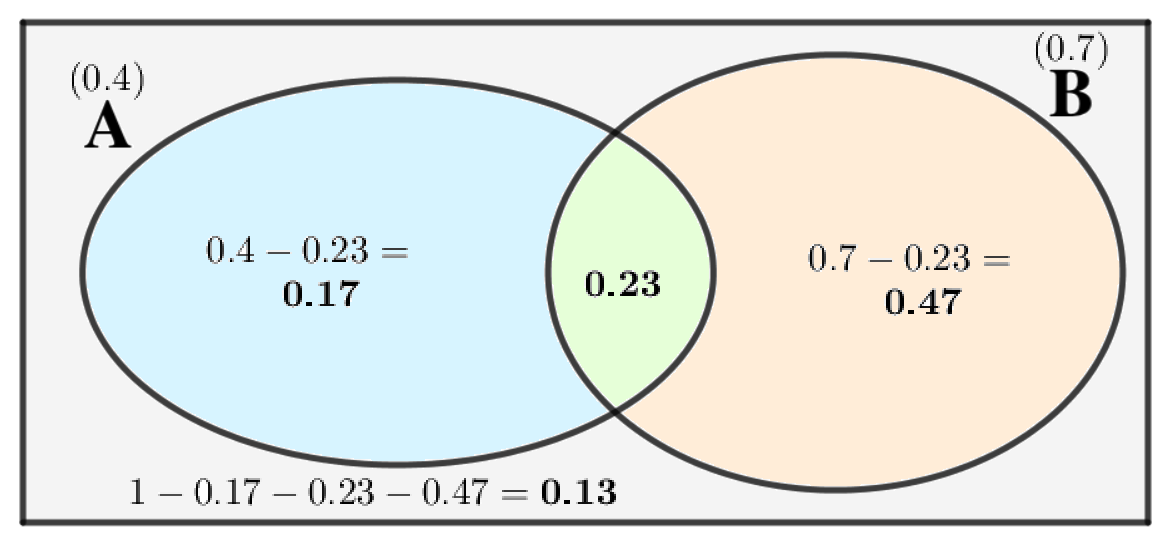
\includegraphics[width=.6\textwidth]{imagenes/imagenes02/T02IM17.png}
	\end{figure}
\begin{small}Colocando $0.23$ en la intersección, la zona azul $A-B$ (gafas pero no ojos marrones) tendrá una probabilidad de $0.4-0.23=0.17$, análogamente encontramos que la probabilidad de que la persona tenga ojos marrones pero no lleve gafas ($B-A$, zona naranja) es $0.47$ y que la probabilidad de que la persona elegida ni tenga ojos marrones ni use gafas, la zona del exterior, será $0.13$, puesto que la probabilidad total ha de ser uno.\end{small}

Sin más que observar el gráfico: 

$a)\ \ p(\text{no lleve gafas})=0.47+0.13=1-0.4=0.6$

$b)\ \ p(\text{use gafas o tenga ojos marrones})=0.17+0.23+0.47=1-0.13=0.87$

$c)\ \ p(\text{lleve gafas pero no tenga los ojos marrones})=0.17$

También podríamos resolver el problema sin necesidad de usar un diagrama de Venn.

$a)\ \ $ No llevar gafas es el suceso contrario a $A$, $A'$. 

Así, $p(A')=1-p(A)=1-0.4=0.6$

$b)\ \ $ Usar gafas o tener ojos marrones es el suceso unión, por ello, 

$p(A\cup B)=p(A)+p(B)-p(A\cap B)=0.4+0.7-0.23=0.87$

$c)\ \ $ Llevar gafas sin tener los ojos marrones es el suceso diferencia, $A-B$. Como los sucesos $A-B$ y $A\cap B$ son disjuntos (zona morada y zona verde), la probabilidad de su unión (el suceso A) es la suma de probabilidades (Axioma 3 de Kolmogorov):

$(A-B) \cap (A\cap B)=\emptyset \to $

$p(\ (A-B) \cup (A\cap B) \ )= p(A) =p(A-B) + p(A\cap B) \to $

$0.4=p(A-B)+0.23 \to p(A-B)=0.17$

\emph{Realmente, el uso del diagrama de Venn simplifica enormemente la resolución del problema.}
\end{ejemplo}
	
\begin{ejemplo}
\begin{ejre}
Una urna contiene 5 bolas azules, 3 rojas y 2 verdes. Consideremos el experimento consistente en extraer de la urna una bola al azar, calcular las siguientes probabilidades:

$a)\ $ Sale bola azul; $b)\ $ la bola extraída no es roja; $c)\ $ sale bola negra; $d)\ $ sale bola azul o verde.	
\end{ejre}

\vspace{4mm} En este caso, los sucesos A='bola azul', R='bola roja' y V=`bola verde' son mutuamente incompatibles por lo que podemos aplicar el axioma 3, pero, resolveremos el problema con la ayuda de un \textbf{\emph{diagrama de árbol}}, lo que facilitará mucho la resolución.	


% Set the overall layout of the tree
\tikzstyle{level 1}=[level distance=7cm, sibling distance=1cm]

% Define styles for bags and leafs
\tikzstyle{bag} = [text width=5.5cm, text centered]

\begin{center}
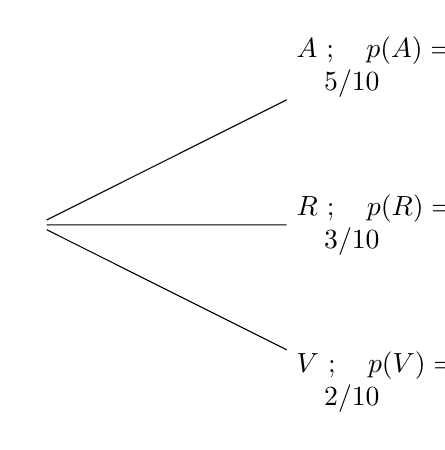
\begin{tikzpicture}[grow=right, sloped]
\node {}
    child {
        node[bag] {$V\ ; \quad p(V)=2/10$}          
    }
    child {
        node[bag] {$R\ ; \quad p(R)=3/10$}              
    }
    child {
        node[bag] {$A\ ;  \quad p(A)=5/10$}              
    }
    ;
\end{tikzpicture}
\end{center}
	
$a)\ p(A)=5/10$

$b)\ p(R')=1-3/10=7/10=5/10+2/10$

$c)\ p(N)=0/10=0$

$d)\ p(A\cup V)=5/10+2/10=7/10 \textcolor{gris}{=p(R')}$
\end{ejemplo}

\begin{ejemplo}
\begin{ejre}
 En un grupo de 40 alunnos hay 22 chicos y 18 chicas. Llevan gafas 8 chicos y 6 chicas. 
 
 a) Elegido un alumno al azar, calcula la probabilidad de que sea chico y no lleve gafas.
 
 b) ?`Cuál es la probabilidad de elegir a una persona con gafas? 
 
c)  Si sabemos que la persona que va a ser elegida es un chico, ?`cuál es ahora la probabilidad de que lleve gafas?
\end{ejre}

\vspace{4mm} Vamos a ver un nuevo tipo de `gráfico' que nos facilitará la resolución del problema, en esta ocasión usaremos una \textbf{\emph{tabla de contingencia}}.

\begin{multicols}{2}
\begin{table}[H]
%\small
\centering
\begin{tabular}{c|c|c|c}
 & chico & chica &  \\ \hline
gafas & \textbf{8} & \textbf{6} & 14 \\ \hline
sin gafas & 14 & 12 & 26 \\ \hline
 & \textbf{22} & \textbf{18} & 40
\end{tabular}
\end{table}
Colocamos, en negrita, los datos del problema y rellenamos los huecos y totales de la tabla.

$a)\ \ p(\text{chico y gafas})=8/40$
\end{multicols}

$b)\ \ p(\text{gafas})=14/10; \quad c)\ \ p(\text{gafas, sabiendo que es chico})=8/14$

Esto nos llevará al siguiente apartado, \emph{probabilidad condicionada}.
	
\end{ejemplo}

\begin{destacado}
	En múltiples ocasiones, un diagrama de Venn, un diagrama de árbol o una tabla de contingencia, que obviamente responda al enunciado del problema, nos facilitará mucho su resolución. Es la experiencia la que determinará que opción usar en cada momento. (En general, el diagrama de árbol se usará para sucesos incompatibles y para pruebas compuestas y el diagrama de Venn o tablas de contingencia se usará para sucesos compatibles).
	
	\emph{En lo que queda de tema, por motivos didácticos, se intentará siempre el uso de estas ayudas y evitar, en lo posible, el excesivo uso de fórmulas}.
\end{destacado}

\begin{ejemplo}
\begin{ejre}\textcolor{gris}{.}

Se sabe que $\ p(A)=0.5$, $p(B')=0.7$ y que $p(A'\cup B')=0.8$. 

Calcular: $p(A\cup B)$;	$p(A\cap B)$; $p(A-B)$ y $p(A'\cap B')$.
\end{ejre}
	\begin{figure}[H]
			\centering
			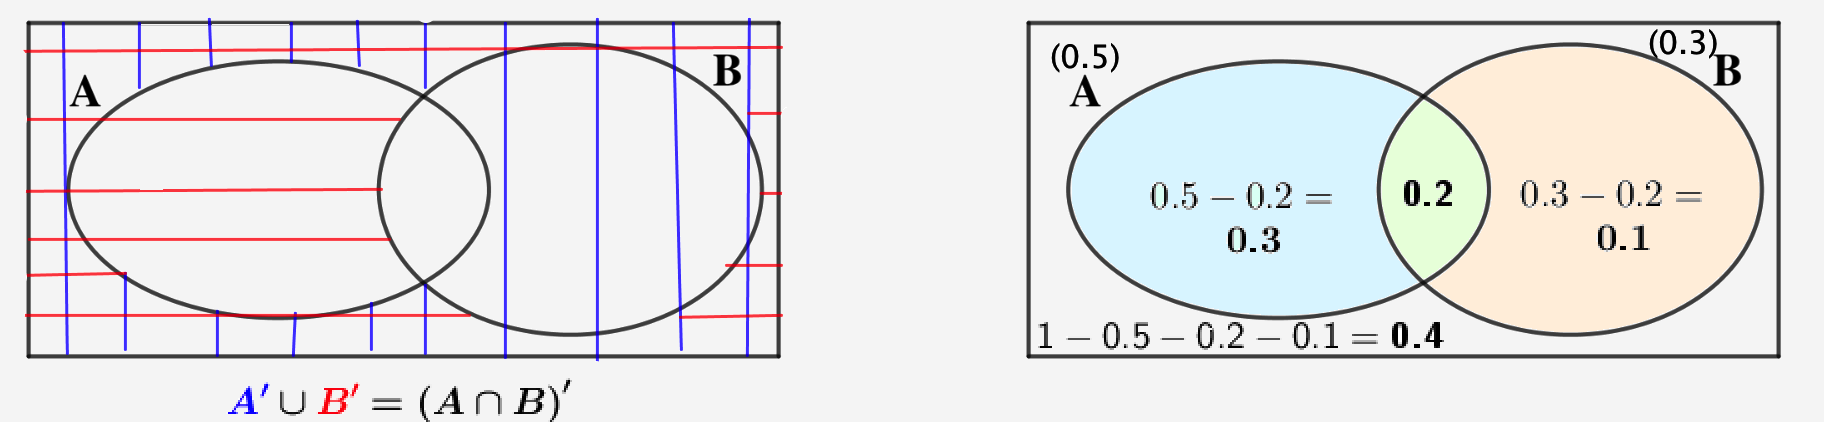
\includegraphics[width=1\textwidth]{imagenes/imagenes02/T02IM18.png}
	\end{figure}
Como $p(B')=0.7 \to P(B)=1-0.7=0.3$

Hemos dibujado con verticales azules $A'$ y con horizontales rojas $B'$, la unión está formada por todas las zonas rayadas de cualquier modo (la intersección donde aparecen las rayas cruzadas). Por ello, vemos que $A'\cup B'=(A\cap B)'$ (Leyes de Morgan), luego $p(A'\cup B')=p(A\cap B)'=1-p(A\cap B)=0.8 \to p(A\cap B)=0.2$

Averiguado esto, es fácil obtener las probabilifades que faltan y aparecen el el segundo diagrama.
\end{ejemplo}


\begin{myexampleblock}{Dominó y barajas (española y francesa)}

\begin{small}
El \textbf{dominó} es un juego de mesa en el que se juegan y emplean unas fichas rectangulares, generalmente blancas por la cara y negras del revés. La cara blanca está dividida por dos cuadrados, cada uno de los cuales está numerado mediante disposiciones de puntos del cero al seis. Hay en total 28 fichas,  $\{(0,0),(0,1),(0,2), \cdots (6,6)\}$
	\begin{figure}[H]
			\centering
			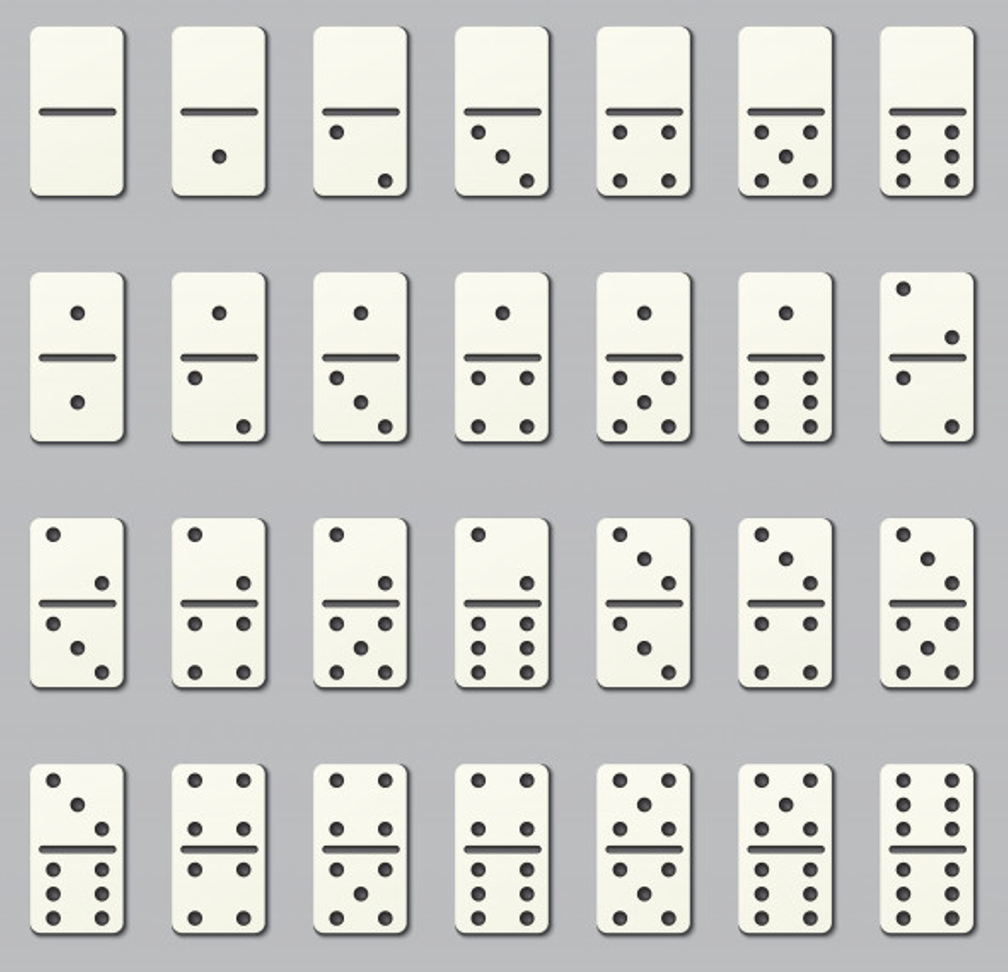
\includegraphics[width=.6\textwidth]{imagenes/imagenes02/T02IM19.png}
	\end{figure}

\vspace{2mm} La \textbf{baraja española} es un mazo o conjunto de cuarenta naipes o cartas de la baraja.  Los naipes están divididos en cuatro ``familias'', ``pintas'' o ``palos''. Los palos son ``oros'', ``copas'', ``espadas'' y ``bastos'', a cada uno de los cuales le corresponde su iconografía característica. Cada palo tiene diez cartas: siete cartas numeradas del uno al siete, llamadas cartas numéricas y tres figuras (sota, caballo y rey) numeradas correlativamente del diez al doce. 
	\begin{figure}[H]
			\centering
			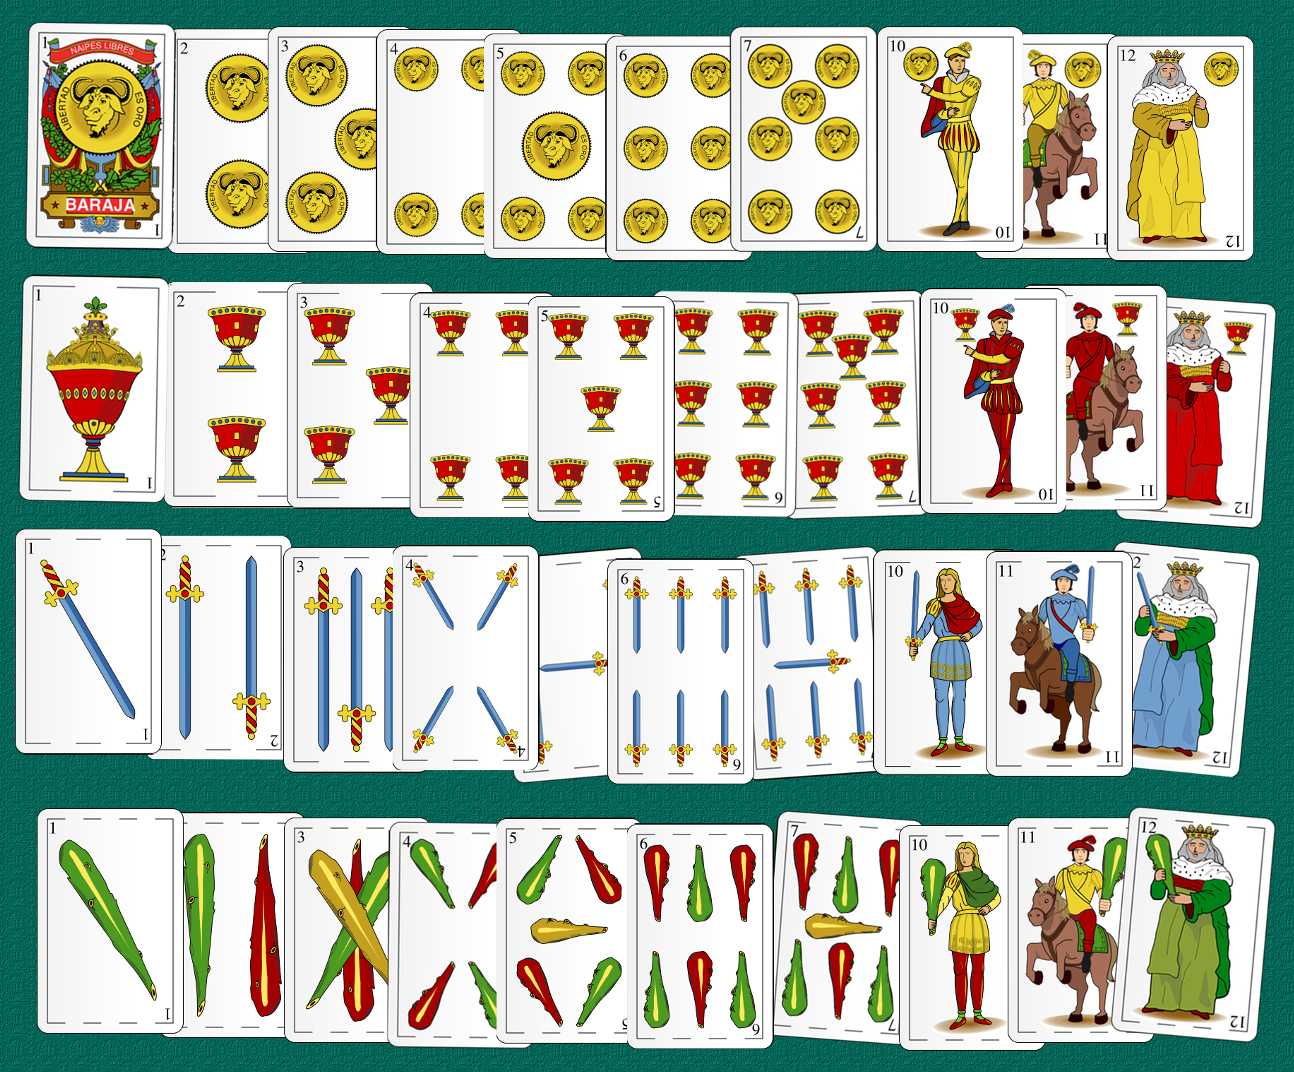
\includegraphics[width=.6\textwidth]{imagenes/imagenes02/T02IM20.png}
	\end{figure}

\vspace{2mm} La \textbf{baraja francesa} es un conjunto de naipes o cartas, formado por 52 unidades repartidas en cuatro palos: corazones, diamantes (que son rojas) , tréboles y picas (que son negras).  Cada palo está formado por 13 cartas, 10 numéricas (del 1 al 10) y tres figuras (sota-Jack, reina-Queen y rey-King: J, Q, K).
	\begin{figure}[H]
			\centering
			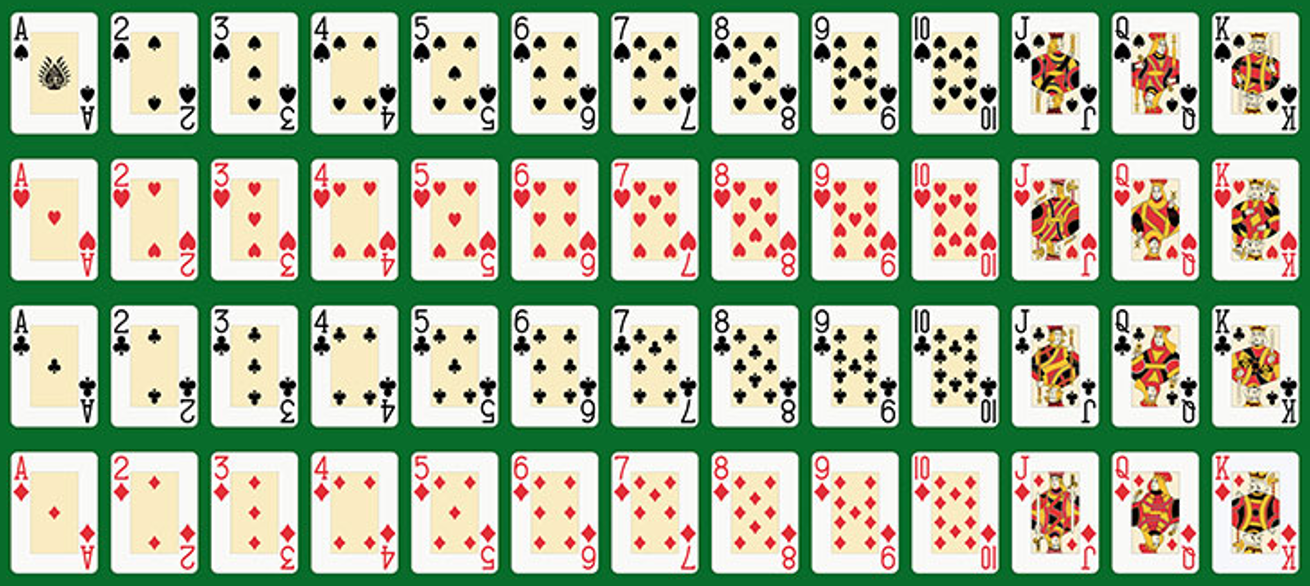
\includegraphics[width=.9\textwidth]{imagenes/imagenes02/T02IM21.png}
	\end{figure}
\end{small}
\end{myexampleblock}


\section{Probabilidad condicionada}	
	
\normalsize{La} \emph{probabilidad condicionada} es uno de los conceptos clave en Teoría de la Probabilidad. Hasta ahora, hemos introducido el concepto de probabilidad considerando que la única información sobre el experimento era el espacio muestral. Sin embargo, hay situaciones en las que se incorpora información suplementaria, como que haya ocurrido otro suceso, con lo que puede variar el espacio de resultados posibles y consecuentemente, sus probabilidades. En este contexto aparece el concepto de probabilidad condicionada. 

El objetivo es analizar cómo afecta el conocimiento de la realización de un determinado suceso a la probabilidad de que ocurra cualquier otro. 

\begin{definition}
.	Se llama \textbf{probabilidad condicionada} de que ocurra el suceso $B$ sabiendo que ha ocurrido el suceso $A$, y se denota por $P(B|A)$ al cociente entre $p(A\cap B)$ y $p(A)$ y \emph{mide las veces que ocurre $B$ de entre las que ocurre $A$.}
	
	$$\subrayado{\ \boxed{\ \boldsymbol{p(B|A)\ = \ \dfrac{p(A\cap B)}{p(A)}} \ } \ }$$
\end{definition}

\emph{La probabilidad de un suceso condicionada a otro es el cociente entre la probabilidad de la intersección y la probabilidad del suceso que condiciona.} \textcolor{gris}{El suceso que condiciona, su probabilidad, va en el denominador.}


\begin{theorem}
. Como la intersección de sucesos es conmutativa, $A\cap B=B\cap A$, se tiene:

$$	\boldsymbol{ p(A\cap B)=p(A)\cdot p(B|A); \qquad \qquad p(A\cap B)=p(B)\cdot p(A|B) } $$
\end{theorem}

\begin{proof}
	Para demostrar la primera expresión no hay más que despejar en la definición de probabilidad condicionada. En la segunda expresión se han intercambiado los papeles de $B$ y $A$.	
\end{proof}

\begin{theorem}
.	$$p(A\cap B\cap C)=p(A)\cdot p(B|A)\cdot p(C|A\cap B)$$	
\end{theorem}

\begin{proof}
$p(	A\cap B\cap C)=p(\ (A\cap B) \ \cap C\ )= p(A\cap B)\cdot p(C|A\cap B) =\ (\to) $

por el teorema anterior, $\ (\to) \ = p(A)\cdot p(B|A) \cdot p(C|A\cap B)$
\end{proof}


\begin{definition}
.	\textbf{Sucesos Dependientes e Independientes}	

\vspace{2mm} Si $p(B|A)=p(B)\ \to \ $ se dice que $A$ y $B$ son \textbf{independientes}. El saber que ha ocurrido $A$ no modifica la probabilidad de que ocurra $B$, el hecho de que ocurra $B$ no se ve influido por la ocurrencia o no de $A$, son \emph{independientes}. 

\vspace{2mm} Si $p(B|A) \neq p(B)\ \to \ $ se dice que $A$ y $B$ son \textbf{dependientes}
\end{definition}

\begin{theorem}
.	Si $A$ es independiente de $B \ \Rightarrow \ B$ es independiente de $A$. 	
\end{theorem}
\begin{proof}
$A$ independiente $B$ $\ \to \ $ $p(A|B)=p(A);\ \ \dfrac{p(A\cap B)}{\textcolor{blue}{p(B)} }= \textcolor{red}{p(A)} \ \to $

$\ \to  \dfrac{p(A\cap B)}{ \textcolor{red}{p(A)}} =  \textcolor{blue}{p(B)};\ \ p(B|A)=p(B) \ \to \ B$ independiente de $A$.	
\end{proof}



\begin{theorem}
. Para sucesos	independientes: $\quad \boldsymbol{ p(A\cap B)=p(A)\cdot p(B)}$
\end{theorem}
\begin{proof}
Evidentemente, al ser $A$ y $B$ independientes, 	$p(B|A)=p(B)$, por lo que al calcular, según la definición, la probabilidad de la intersección:
$p(A\cap B)=p(A)\cdot p(B|A) = p(A)\cdot p(B)$
\end{proof}

\begin{destacado}
También se puede tomar este hecho como comprobación de si dos sucesos son o no independientes:
 
$$ \boldsymbol{ A \textbf{ y } B \textbf{ son independientes } \ \ \longleftrightarrow \ \ p(A\cap B)=p(A)\cdot p(B) }  $$	
\end{destacado}

\begin{destacado}
Atención: no se debe confundir sucesos \textbf{independientes} con sucesos \textbf{incompatibles}:	

--- Si $\  \boldsymbol{ p(B|A)=p(B)\ \to \ }$ se dice que $A$ y $B$ son \textbf{independientes}.

--- Si $\  \boldsymbol{ p(A\cap B)=0 \ \ \to \ }$ se dice que $A$ y $B$ son \textbf{incompatibles}.

\end{destacado}

Podemos reconocer que nos preguntan por una probabilidad condicionada, $p(B|A)$, y no por una normal, $p(B)$ por el enunciado, que será de la forma:

\begin{itemize}
\vspace{-2mm} \item Calcula la probabilidad de B condicionada a A.
\vspace{-2mm} \item Calcula la probabilidad de B \emph{sabiendo} que ha ocurrido A.	
\vspace{-2mm} \item \emph{Sabiendo} que ha ocurrido A, calcula la probabilidad de que ocurra B.
\end{itemize}
\vspace{-2mm} \textcolor{gris}{\emph{!`Ojo a los subjuntivos!}}

\begin{example}
.	De una baraja de 40 cartas española, se extrae una carta al azar. Calcular: 

a) la probabilidad de que sea figura (sota, caballo o rey).

b) la probabilidad de que sea rey.

c) sabiendo que la carta extraída es figura, ?`cuál es la probabilidad de que sea rey?

d) sabiendo que la carta extraída es de copas, ?`cuál es la porb. de que sea rey?

e) ?`Son independientes los sucesos “la carta es rey” y “la carta es figura”? ?`Y los sucesos “la carta es rey” y “la carta es de copas”? 	

\vspace{4mm}

Llamamos F=``la carta es figura''; R=``la carta es rey''; Co=``la carta es de copas''.

$a)\quad p(F)=(3\cdot 4)/40=3/10=0.30$

$b)\quad p(R)=4/40=0.10$

$c)\quad p(R|F)=0.33$

--- con fórmula, $p(R|F)=\dfrac{p(R\cap F)}{p(F)}=\dfrac{4/40}{12/40}=4/12=1/3=0.33$

--- directamente, de la definición: probabilidad sacar un rey (hay 4) sabiendo que el sorteo se efectúa entre las figuras (son 12), entonces, $p(R|F)=4/12=1/3=0.33$. !`Más fácil!

$d)\quad p(R|Co)=1\text{(el rey de copas)}/10\text{(copas)}=0.10$

$e)\quad$ Dependencia e independencia de los sucesos R con $F$ y $co$:

--- $\ R$ y $F$: $\ \ p(R|F)=0.33 \neq 0.10 = p(R) \to $ $F$ y $R$ son \emph{dependientes}.

--- $\ R$ y $Co$: $\ p(R|Co)=0.10 = p(R) \to $ $R$ y $Co$ son \emph{independientes}.

Es decir, el hecho de saber o no que la carta a extraer va a ser de copas no afecta a la probabilidad de sacar un rey, en cambio; si sabemos que la extracción va a ser sobre las figuras, si cambia (aumenta en este caso) la probabilidad de sacar rey.

\emph{La información modifica la probabilidad.}

\end{example}


\section{Teorema de la probabilidad total y teorema de Bayes}
Se llaman \textbf{pruebas compuestas o experiencias compuestas} a aquellas en las que se pueden distinguir dos o más etapas.

El desarrollo de los sucesos de una experiencia compuesta se puede representar con un \textbf{diagrama en árbol}.

El diagrama de árbol es una representación gráfica de los posibles resultados del experimento, el cual consta de una serie de pasos, donde cada uno de estos tiene un número infinito de maneras de ser llevado a cabo. Se utiliza en los problemas de conteo y probabilidad.

Para la construcción de un diagrama en árbol se partirá poniendo una rama para cada una de las posibilidades, acompañada de su probabilidad. Cada una de estas ramas se conoce como rama de primera generación.

En el final de cada rama de primera generación se constituye, un nudo del cual parten nuevas ramas conocidas como ramas de segunda generación, según las posibilidades del siguiente paso, salvo si el nudo representa un posible final del experimento (nudo final).

\begin{destacado}
Hay que tener en cuenta que la suma de probabilidades de las ramas de cada nudo ha de dar siempre 1.	
\end{destacado}

Las probabilidades de los sucesos finales (intersección de las ramas que conducen a ellos) se obtiene multiplicando las probabilidades de las ramas.

	
\begin{definition}
. Un \textbf{Sistema Completo de Sucesos} es una serie de sucesos $A_1, A_2, \cdots A_n$ que cumplen:

$$A_1\cup A_2 \cup \cdots \cup A_n=\displaystyle \cup_{i=1}^n A_i=E;\qquad A_i\cap A_j=\emptyset,\ \forall i\neq j;\qquad p(A_i)\neq 0,\ \forall i$$	

\begin{figure}[H]
			\centering
			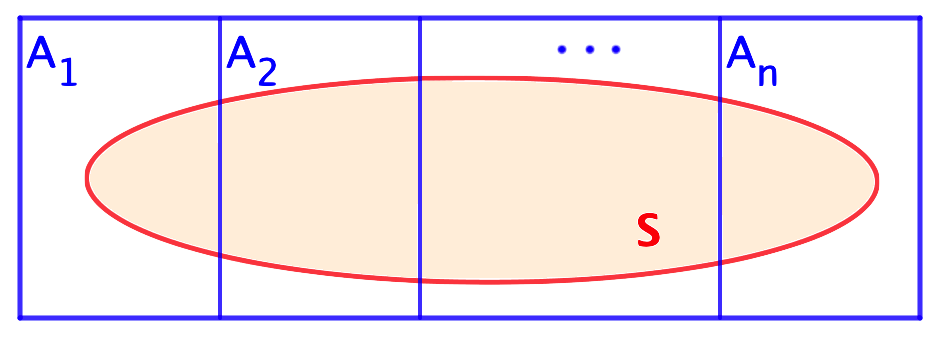
\includegraphics[width=.6\textwidth]{imagenes/imagenes02/T02IM22.png}
	\end{figure}
\end{definition}

\begin{theorem}
.	\textbf{Teorema de la probabilidad total}	

Si $S$ es un suceso cualquiera y $A_i,\ 1\le i\le n$ es un sistema completo de sucesos, se cumple:

$$\boldsymbol{ p(S)=  p(S|A_1)\cdot p(A_1)+ p(S|A_2)\cdot p(A_2) + \cdots + p(S|A_n) \cdot p(A_n)}$$
\end{theorem}

\begin{proof}\textcolor{white}{.}

$A_1\cup A_2 \cup \cdots \cup A_n=E	 \to S=S\cap E=S\cap A_1 \ \cup \ S\cap A_2 \ \cup \cdots \cup \ S\cap A_n$, todos disjuntos (al serlo los $A_i$), por lo que, por el Axioma 3 de Kolmogorov, 
$p(S)=\displaystyle \sum_{i=1}^n \ p(S\cap A_i) = p(A_1\cap S)+p(A_2\cap S)+ \cdots + p(A_n\cap S) = p(S|A_1)\cdot p(A_1)+ p(S|A_2)\cdot p(A_2) + \cdots + p(S|A_n) \cdot p(A_n)$

\textcolor{gris}{La intersección de sucesos es conmutativa: $\ A_i\cap S=S\cap A_i, \ \forall i$}
\end{proof}


Este teorema proporciona una forma de obtener la probabilidad (total) de un suceso de la segunda (o última) etapa de la experiencia compuesta sin condicionar a ninguno de la primera. En un diagrama de árbol, basta con sumar las probabilidades de las ramas finales en que se verifica el suceso en cuestión. (Ver ejemplo siguiente).

\begin{theorem}
.	\textbf{Teorema de Bayes}	

Si $S$ es un suceso cualquiera y $A_i,\ 1\le i\le n$ es un sistema completo de sucesos, se cumple, que para cada suceso $A_i$,

$$ \boldsymbol{ p(A_i|S) \ = \  \dfrac{p(A_i)\cdot p(S|A_i)} { p(S|A_1)\cdot p(A_1)+ p(S|A_2)\cdot p(A_2) + \cdots + p(S|A_n) \cdot p(A_n)}  }$$
\end{theorem}

\begin{proof}\textcolor{white}{.}

$ p(A_i|S)   = \dfrac{p(A_i\cap S)}{p(S)} = 
\dfrac{ p(S) \cdot p(A_i) } { p(S) }  	$ , solo queda aplicar el teorema de la probabilidad total en el denominador.

\textcolor{gris}{La intersección de sucesos es conmutativa: $\ A_i\cap S=S\cap A_i, \ \forall i$}
\end{proof}


Este teorema proporciona el cálculo de probabilidades `a posteriori', es decir, conocer la probabilidad de un suceso de la primera etapa condicionado (sabiendo) que ha ocurrido determinado suceso de la segunda etapa.  En un diagrama de árbol, basta con observar todos los sucesos que verifican el suceso de la segunda etapa  (posibles) y aquel o aquellos de éstos que verifican el suceso de la primera etapa (favorables) y, ahora, aplicar la regla de Laplace.(Ver ejemplo siguiente).

\begin{example}
	. Tenemos tres urnas. La primera contiene 4 bolas rojas y 4 negras; la segunda, 3 rojas y 1 negra, y la tercera, 2 rojas y 4 negras. Elegimos una urna al azar y sacamos una bola de ella.
	
	Calcula la probabilidad de que la bola extraída haya sido negra.
	
	Sabiendo que la bola extraída es negra, ?`cuál es la probabilidad de que sea de la urna 3.
	
	\vspace{4mm} Tenemos una experiencia compuesta. En la primera parte elegimos, al azar, una urna (todas tienen la misma probabilidad de ser elegidas, cada una de ellas $p(U_i)=1/3$). La segunda parte consiste en extraer una bola de la urna, que puede ser roja o negra con probabilidades $p(R)$ y $p(N)$ distintas según la urna de la que se trate.

	\begin{figure}[H]
			\centering
			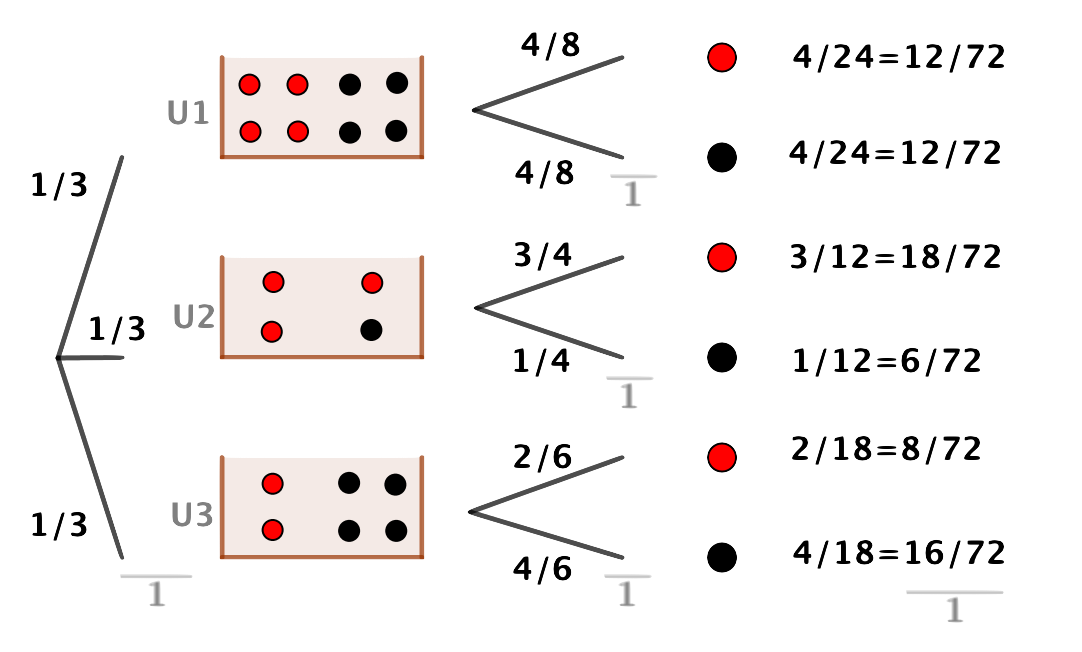
\includegraphics[width=.75\textwidth]{imagenes/imagenes02/T02IM23.png}
	\end{figure}	
	
Las probabilidades de los sucesos compuestos se obtienen multiplicando las ramas que conducen a ellos: p(urna 1 y bola negra)$=p(U1 \cap N)=\dfrac 1 3 \cdot \dfrac 4 8 = \dfrac 4  {24}$. Una de cada tres veces vamos a la urna uno; una vez allí, cuatro de cada ocho veces sacamos bola negra, luego  $\dfrac 1 3 \cdot \dfrac 4 8 = \dfrac 4 {24}$, es decir, cuatro de cada veinticuatro veces habremos ido a la urna 1 y sacado bola roja.  Obtenemos las \emph{probabilidades de los sucesos compuestos multiplicando las probabilidades de las ramas de donde provienen}.

\vspace{2mm} Presentamos las probabilidades finales (de los sucesos compuestos) reducidas a común denominador para mayor claridad del problema.

\vspace{2mm} \textbf{Probabilidad de que la bola extraída haya sido negra}: Si nos fijamos en el árbol, la bola extraída es negra en 12 de cada 72 veces (U1), también en 6 de cada 72 veces (U2) y en 16 de cada 72 veces, en total, en 12+6+16=34 de cada 72 veces. Esto nos permite concluir que $p(N)=34/72$

\vspace{2mm} Hemos calculado la probabilidad de un suceso de la segunda etapa (la bola es negra) sin condicionar a ninguno de la primera etapa (U1, U2, U3): tenemos un \textbf{Teorema de la Probabilidad Total}, hemos, simplemente, \emph{sumado todas las probabilidades que conducen a ese suceso}.

\vspace{2mm} \textcolor{gris}{Usando fórmulas, $P(N)=p(U1)\cdot p(N|U1)+p(U2)\cdot p(N|U2)+p(U1)\cdot p(N|U3)=\frac 1 3 \cdot \frac 4 8 + \frac 1 3 \cdot \frac 1 4 + \frac 1 3 \cdot \frac 4 6 = \frac{34}{72}$}

\vspace{2mm} \textbf{Probabilidad de haber ido a la urna 3 sabiendo que la bola extraída es negra}. Los caso posibles de extraer bola negra son $12/72,\ 6/72 \text{ y } 16/72$, de ellas solo en $16/72$ ocasiones hemos ido a la urna 3 (casos favorables), sin más que usar la regla de Laplace, concluimos que $p(U3|N)=\dfrac{16/72}{12/72 + 6/72 + 16/72}=\dfrac{16/72}{34/72}=\dfrac {16}{34} $ \textcolor{gris}{$\approx 47\%>33\%$} \textcolor{gris}{como decía la intuición, en la urna tres es más probable sacar bola negra que en las otras.}

\vspace{2mm} Hemos calculado una probabilidad de la primera etapa (U3), condicionado a un suceso de la segunda etapa (N), esto es un \textbf{Teorema de Bayes}, tan solo hemos aplicado la regla de Laplace: \emph{favorables/posibles}. 

\vspace{2mm} \textcolor{gris}{Usando fórmulas, $P(U3|N)=\dfrac{p(U3)\cdot p(N|U3)}{p(N)}=\dfrac {1/3 \cdot 4/3}{34/72}\approx 47\%$}

\vspace{4mm}\textsf{Como se puede comprobar, se pueden resolver problemas de ambos teoremas tan solo con un buen árbol y sabiendo que es lo que nos preguntan, huyendo de las fórmulas. Intentaremos resolver así la mayoría de los problemas.}

\vspace{2mm} \textsl{Nótese que, como hemos comprobado en el árbol, todas las ramas que parten de un nodo, sus probabilidades suman UNO. Así como las probabilidades de las hojas finales.}
\end{example}

Presentamos algunos ejercicios resueltos más, usando todos los métodos: árbol, Venn y tablas contingencia. Unos son más sencillos y directos que otros, que requieren cáculos adicionales.

\begin{example}
. \begin{ejre}
	La probabilidad de que una detreminada enfermedad aparezca en un individuo es del 3\%. De entre los enfermos, el 15\% tienen antecedentes familiares y el 2\% de los que no están enfermos también tienen antecedentes familiares. Calcular:
	
	\vspace{2mm} a) porbabilidad de que una persona de esa ciudad no tenga antecedentes familiares.
	
	\vspace{2mm} b) probabilidad de que una persona que no tenga antecedentes familiares \textcolor{gris}{(sabiendo que la persona no tiene antecedentes familiares)}, no padezca la enfermedad.
	
	\vspace{2mm} c) tener la enfermedad y tener antecedentes familiares, ?`son sucesos incompatibles?, ?`e independientes?

\vspace{4mm} $\boldsymbol{\Rightarrow}\quad $ \textbf{Árbol}.
	
\begin{multicols}{2}
	\begin{figure}[H]
			\centering
			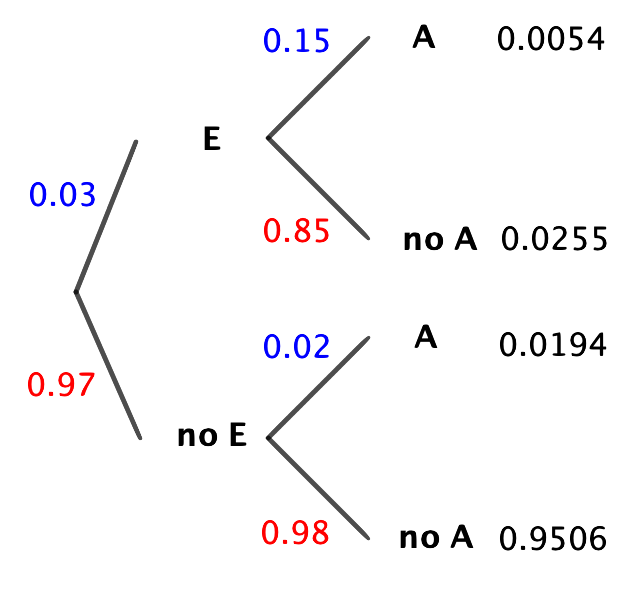
\includegraphics[width=.5\textwidth]{imagenes/imagenes02/T02IM24.png}
	\end{figure}
	Llamamos $E$ al suceso `la persona está enferma', $no\ E$ a su suceso contrario, $A$ a `la persona tiene antecedentes' y $no\ A$ a su contrario.
	
	Una persona cualquiera puede estar o no $E$ y, después, puede que tenga  o no $A$.
	
	Hemos colocado en las ramas los valores conocidos, en azul. En rojo aparecen las probabilidades de los contrarios, sin más que recordar que en un árbol ``las probabilidad de todas las ramas debe sumar uno''.
\end{multicols}		
	
a) $\ p(no \ A)=0.0255+0.9506=0.9761$

b) $\ p(no \ E|no \ A)=\dfrac f p =\dfrac{0.9506}{0.0255+0.9506}=0.9739$

d) $\ p(no \ E|no \ A)=0.9739\neq 0.97=p(no \ E) \to no\ E \ \wedge \ no \ A $ son dependientes, luego $E$ y $A$ también dependientes.

$p(no \ E \text{ y } no \ A)=0.9506\neq 0 \to no\ E \ \wedge \ no \ A$ son compatibles, y también $E$ y $A$ son compatibles. ($\ p(E\cap A)=0.054\neq 0\ $). 

\vspace{4mm} $\boldsymbol{\Rightarrow}\quad $ \textbf{Diagrama de Venn}.

	\begin{figure}[H]
			\centering
			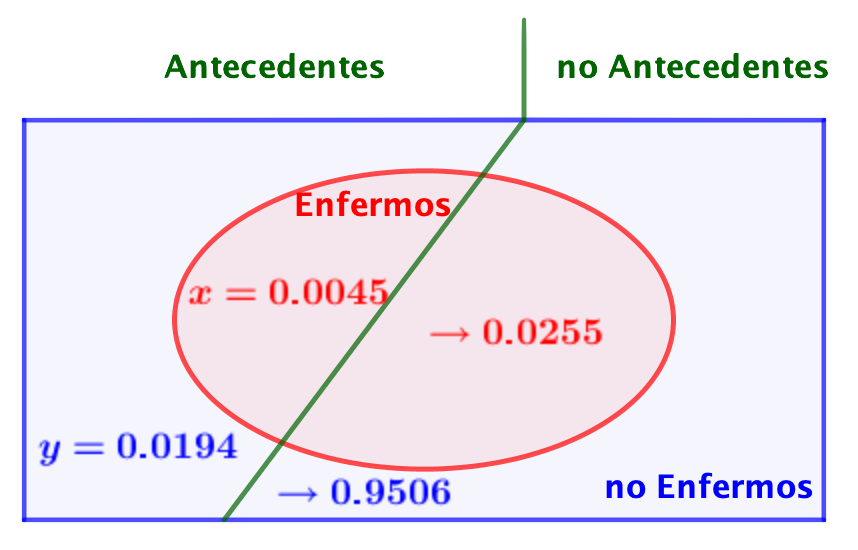
\includegraphics[width=.6\textwidth]{imagenes/imagenes02/T02IM25.png}
	\end{figure}


El problema no es directamente abordable por un diagrama de Venn, a no ser que lo preparemos antes.

Puestos que enfermos hay el 3\%=0.03, dentro de la zona roja, $E$, haremos que el total sea 0,03.

Llamando $x=p(E \cap A)=p(E)\cdot p(A|E)=0.03\cdot 0.14=0.0045$. Así, en la zona roja que falta pondremos $0.03-0.0045=0.0255=p(E\cap no\ A)$.

En la zona azul están los $no\ E$, en total han de ser 0.97 (100\%-3\%). Llamando $y=p(no\ E \cap A)=p(no\ E)\cdot p(A|no\ E)=0.97\cdot 0.02=0.0104$. A la derecha pondremos $0.97-0.0194=0.9506=p(no\ E\cap no\ A)$.

Ahora, ya podemos resolver el problema:

a) $\ p(no \ A)=0.0255+0.9506=0.9761$

b) $\ p(no\ E|no\ A)=\dfrac{0.9506}{0.0255+0.9506}=0.9739$

c) de modo análogo a lo resuelto en el árbol, los sucesos $E$ y $A$ son dependientes y compatibles. 

\vspace{4mm} $\boldsymbol{\Rightarrow}\quad $ \textbf{Tabla de contingencia}.
	
\begin{multicols}{2}	
\begin{table}[H]
\centering
\begin{tabular}{c|c|c|c}
 & \textbf{Ant} & \textbf{no Ant} & \textbf{} \\ \hline
\textbf{E} & x=0.0045 & 0.0255 & \textbf{0.03} \\ \hline
\textbf{no E} & y=0.0149 & 0.9506 & \textbf{0.97} \\ \hline
\textbf{} & 0.0194 & 0.9769 & 
\end{tabular}
\end{table}
También necesitamos cálculos previos para abordar el problema mediante uuna tabla de contingencia.
\end{multicols}

$p(A|E)=0.15=\dfrac{p(A\cap E)}{p(E)}=\dfrac{x}{0.03} \to x=0.045$

$p(A|no\ E)=0.02=\dfrac{p(A\cap no\ E)}{p(no\ E)}=\dfrac{y}{0.97} \to y=0.0194$

Calculadas $x$ e $y$, completamos las celdas adyacentes viendo las sumas parciales (en negrita en la tabla). Completamos la fila de abajo sin mas que sumar.

Con la tabla acabada, ya podemos resolver el problema:

a) $\ p(no \ A)=0.9761$

b) $\ p(no \ E | no\ A)=	\dfrac{0.9506}{0.9761}=0.9739$

c) de modo análogo a lo resuelto en el árbol, los sucesos $E$ y $A$ son dependientes y compatibles.
\end{ejre}	
\end{example}


\begin{example}
. \begin{ejre}
 	Una población está formada, a partes iguales, por hombres ($H$) y mujeres ($M$). La probabilidad de que una persona de esa población no lea ningún periódico ($no\ L$) es $0.25$. Además, el porcentaje de individuos o bién lee algún periódico ($L$) o bien es hombre es del $95\%$. Se elige una persona al azar, calcula:
 	
 	$a)\ \ p(H\cap L);\quad b)\ \ p(L|H);\quad c)\ \ $ ?`$H \text{ y } L $ son dependientes?, ?`compatibles?.
 \end{ejre}
 
\vspace{4mm} $\boldsymbol{\Rightarrow}\quad $ \textbf{Diagrama de Venn}. \textcolor{gris}{( Llamamos $\ x=p(H\cap L)\ $ )}
 \begin{figure}[H]
				\centering
			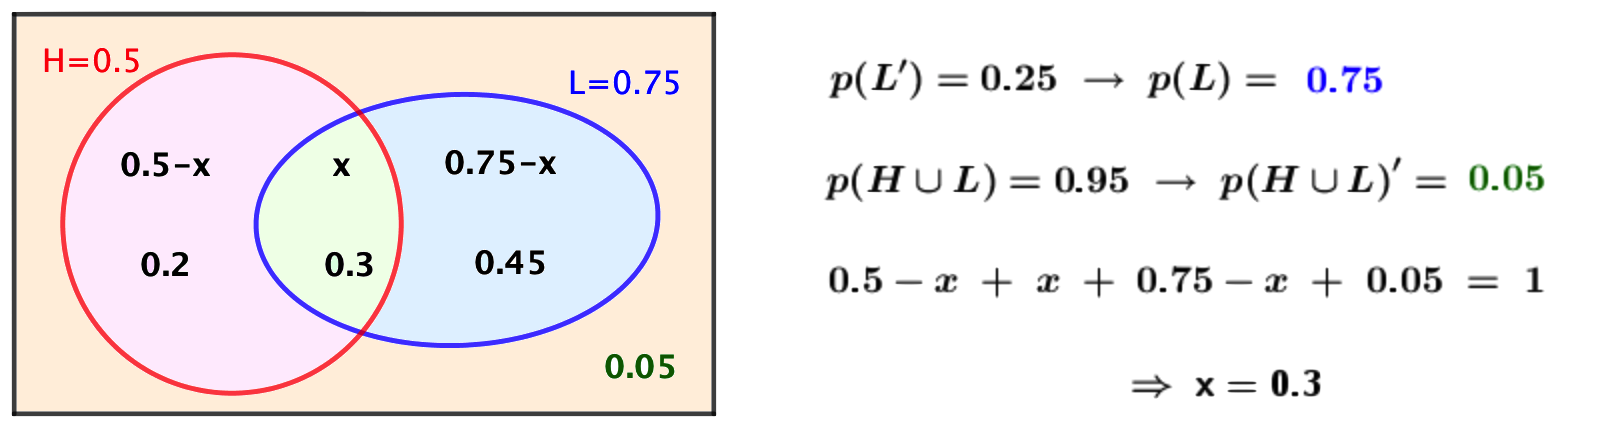
\includegraphics[width=.95\textwidth]{imagenes/imagenes02/T02IM26.png}
	\end{figure}
$p(H\cap L)=0.3\neq 0\to$ Compatibles;

\vspace{2mm} $p(L|H)=\dfrac{0.3}{0.5}=0.6\neq 0.75=p(L)\to $ Dependientes	

\vspace{4mm} $\boldsymbol{\Rightarrow}\quad $ \textbf{Tabla de contingencia}.
\begin{multicols}{2}
\begin{table}[H]
\centering
\begin{tabular}{c|c|c|c}
 & \textbf{H} & \textbf{M} & \textbf{} \\ \hline
\textbf{L} & \begin{tabular}[c]{@{}c@{}}x\\ \\ 0.3\end{tabular} & \begin{tabular}[c]{@{}c@{}}0.75-x\\ \\ 0.45\end{tabular} & \textbf{0.75} \\ \hline
\textbf{no L} & \begin{tabular}[c]{@{}c@{}}0-5-x\\ \\ 0.2\end{tabular} & 0.05 & 0.25 \\ \hline
\textbf{} & \textbf{0.5} & 0.5 & \textbf{1}
\end{tabular}
\end{table}
Llamamos $x=p(H\cap L)$

$\quad$

$p(H\cup L)=x+0.75-x+0.5-x=0.95$

$\quad$

$\to \ \boldsymbol{x=0.3}$

$\quad$

Completamos la tabla.
\end{multicols}
$p(H\cap L)=0.3\neq 0 \to $ compatibles.

\vspace{2mm} $p(L|H)=\dfrac{0.3}{0.5}=0.6\neq 0.75=p(L)\to$ dependientes.

\vspace{4mm} $\boldsymbol{\Rightarrow}\quad $ \textbf{Árbol}.
El problema no directamente abordable desde un árbol, por lo que tendremos que hacer unos cálculos previos.

	\begin{figure}[H]
				\centering
			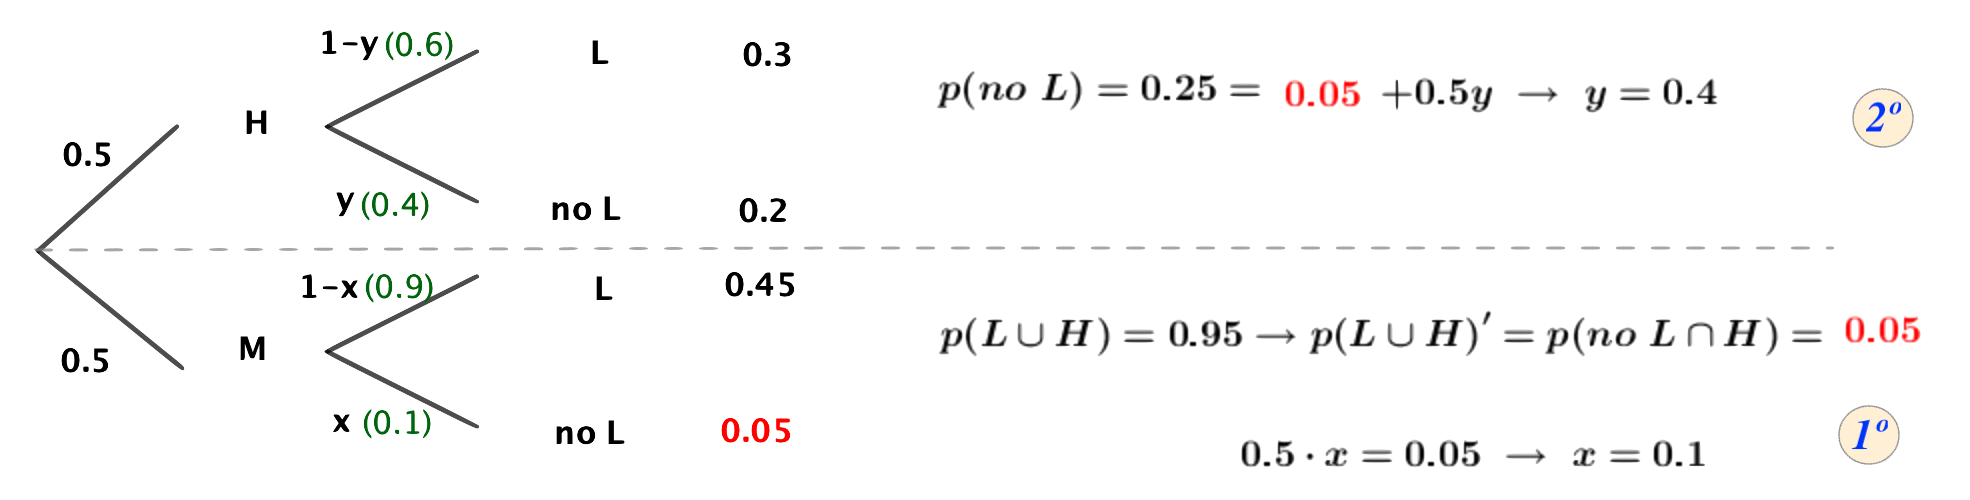
\includegraphics[width=1\textwidth]{imagenes/imagenes02/T02IM27.png}
	\end{figure}
	
$p(H\cap L)=0.3\neq 0 \to $ compatibles.

\vspace{2mm}  $p(L|H)=1-y=0.6\neq 0.75 =0.3+0.45=p(L)\to $ dependientes.


\vspace{4mm} $\boldsymbol{\Rightarrow}\quad $ \textbf{Teóricamente (fórmulas)}.
	
$p(H)=p(M)=0.5;\quad P(no \ L)=0.25 \to p(L)=0.75$

\vspace{2mm}  $p(H\cup L)=p(H)+p(L)-p(H\cap L) \ \to \ 0.95=0.5+0.75-p(H\cap L) \to $

\vspace{2mm}  $\to p(H\cap L)=0.3 \neq 0\to $ comparibles.

\vspace{2mm} $p(L|H)=\dfrac{p(H\cap L)}{p(H)}=\dfrac{0.3}{0.5}=0.6\neq 0.75=p(L) \to $ dependientes.
\end{example}

Con estos ejercicios resueltos queremos poner de manifiesto que de las cuatro estrategias para la resolución de problemas de probabilidad (árbol, Venn, contingencia y fórmulas), en cada problema habrá una más adecuada que otra aunque, con los cálculos necesarios, todas pueden ser útiles. Es la experiencia, tras la realización de muchos ejercicios, la que dirá que método es mejor y más rápido usar. De todos modos, se recomienda que los ejercicios del siguiente apartado se intenten hacer usando distintas estrategias.

En el siguiente cuadro esquematizamos estas cuatro estrategias.


\begin{myalertblock}{Estrategias para la resolución de los problemas de probabilidad}

 $\boldsymbol{\Rightarrow}\quad $ \textbf{Árbol}.

\begin{destacado}
% Set the overall layout of the tree
\tikzstyle{level 1}=[level distance=3.5cm, sibling distance=5.5cm]
\tikzstyle{level 2}=[level distance=3.5cm, sibling distance=3cm]

% Define styles for bags and leafs
\tikzstyle{bag} = [text width=4em, text centered]
\tikzstyle{end} = [circle, minimum width=3pt,fill, inner sep=0pt]

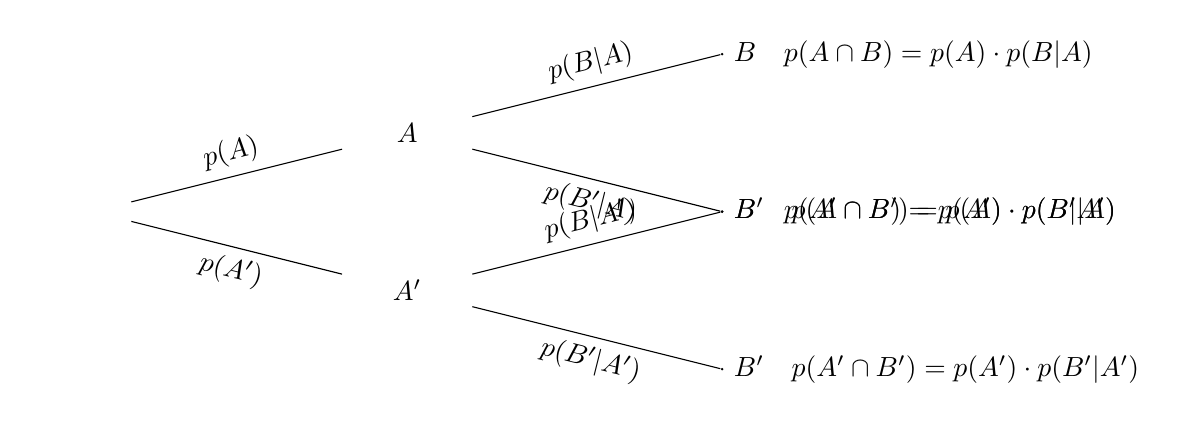
\begin{tikzpicture}[grow=right, sloped]
\node[bag] {}
    child {
        node[bag] {$\boldsymbol{A'}$}        
            child {
                node[end, label=right: {$\boldsymbol{B'}\ \ \  p(A'\cap B')=p(A')\cdot p(B'|A')$}] {}
                edge from parent
                node[above] {}
                node[below]  {$p(B'|A')$}
            }
            child {
                node[end, label=right: {$\boldsymbol{B}\quad p(A'\cap B)=p(A')\cdot p(B|A')$}] {}
                edge from parent
                node[above] {$p(B|A')$}
                node[below]  {}
            }
            edge from parent 
            node[above] {}
            node[below]  {$p(A')$}
    }
    child {
        node[bag] {$\boldsymbol{A}$}   
            child {
                node[end, label=right: {$\boldsymbol{B'}\quad p(A\cap B')=p(A)\cdot p(B'|A)$}] {}
                edge from parent
                node[above] {}
                node[below]  {$p(B'|A)$}
            }
            child {
                node[end, label=right: {$\boldsymbol{B}\quad p(A\cap B)=p(A)\cdot p(B|A)$}] {}
                edge from parent
                node[above] {$p(B|A)$}
                node[below]  {}
            }
            edge from parent         
            node[above] {$p(A)$}
            node[below]  {}
    };
\end{tikzpicture}	
\end{destacado}

$\boldsymbol{\Rightarrow}\quad $ \textbf{Diagrama de Venn}.

\begin{destacado}
	\begin{figure}[H]
				\centering
			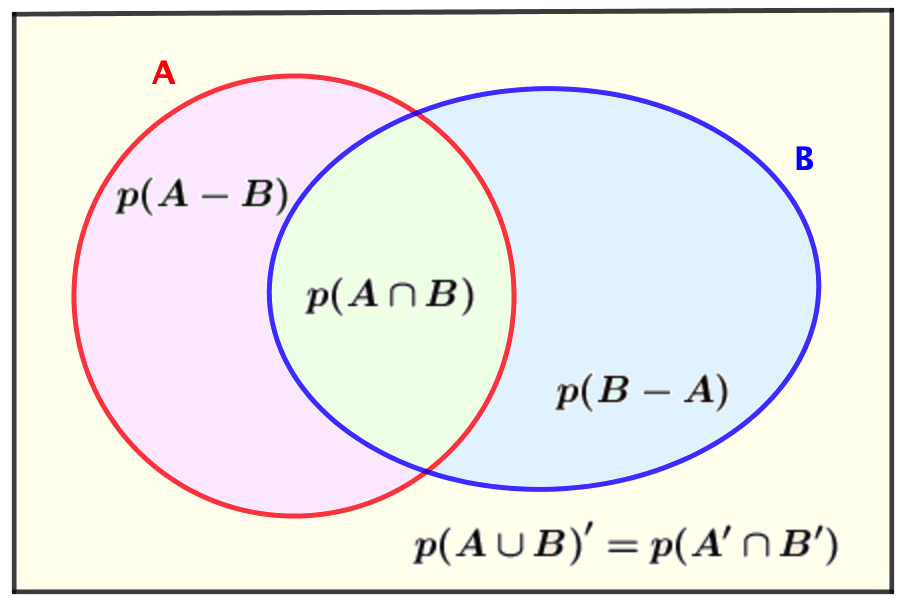
\includegraphics[width=.55\textwidth]{imagenes/imagenes02/T02IM28.png}
	\end{figure}	
\vspace{-9mm}%****************************
\end{destacado}
	
$\boldsymbol{\Rightarrow}\quad $ \textbf{Tabla de contingencia}.
\begin{destacado}

\begin{table}[H]
\centering
\begin{tabular}{c|c|c|c}
 & \textbf{suceso B} & \textbf{suceso B'} & \textbf{totales} \\ \hline
\textbf{suceso A} & $p(A\cap B)$ & $p(A\ \cap B')$ & $\Sigma$ \\ \hline
\textbf{suceso A'} & $p(A'\cap B)$ & $p(A'\cap B')$ & $\Sigma$ \\ \hline
\textbf{totales} & $\Sigma$ & $\Sigma$ & \textbf{1}
\end{tabular}
\end{table}
\vspace{-9mm}%****************************
\end{destacado}

\vspace{4mm} $\boldsymbol{\Rightarrow}\quad $ \textbf{Teóricamente (fórmulas)}.

\begin{destacado}
	Axiomática de Kolmogorov y definición y teoremas de probabilidad condicionada, probabilidad total y teorema de Bayes.
\end{destacado}

\end{myalertblock}

\section{Ejercicios}

$$\subrayado{\  \boxed{ \textbf{Se deberían intentar resolver los ejercicios antes de ver su resolución.} \ } \ }$$

\begin{ejemplo}
\begin{ejer}\textcolor{white}{.}

Una urna 1 tiene tres bolas rojas y dos negras, una urna 2 tiene dos rojas y tres negras.

\begin{adjustwidth}{10mm}{4mm}
A. Nos dirigimos a una urna al azar y sacamos, también al azar, una bola, miramos su color, la devolvemos a la urna y, al azar, sacamos otra bola para observar su color.	(Extracciones con reinserción).

B. Nos dirigimos a una urna al azar y sacamos dos bolas para observar sus colores. (Extracciones sin reinserción).

C. Nos dirigimos a la urna 1 y sacamos una bola, luego nos dirigimos a la urna 2 y sacamos una segunda bola, observando los colores de las bolas extraídas.

D. Nos dirigimos a la urna 1, sacamos una bola para observar su color y la introducimos en la urna 2. Luego, al azar, extraemos una bola de la urna 2 para observar su color.
\end{adjustwidth}


Calcúlese, en cada caso:

\begin{adjustwidth}{10mm}{4mm}
a) Probabilidad de que las dos bolas sean negras.

b) Probabilidad de que las bolas extraídas sean de distinto color.

c) Sabiendo que la bola extraída en segundo lugar en negra, probabilidad de que también lo haya sido la primera bola extraída.
\end{adjustwidth}	
\end{ejer}
\end{ejemplo}

\vspace{20mm}%**********************************
Llamamos $U1,\ U2$ a las urnas; $R1,\ N1$ a los sucesos `la primera bola extraída es roja/negra' y $R2,\ N2$ a los sucesos `la segunda bola extraída es roja/negra'.

Presentamos un diagrama de árbol para cada caso. Se debería estar seguro de la disposición de las ramas y de las probabilidades de cada una de ellas. También se debe comprobar que todas las ramas (incluidas las finales --hojas--) suman uno.




\vspace{40mm}%**********************************
\textcolor{blue}{A. Elegimos urna al azar y sacamos dos bolas con reinserción.}

\vspace{20mm}%**********************************

% Set the overall layout of the tree
\tikzstyle{level 1}=[level distance=3.5cm, sibling distance=7cm]
\tikzstyle{level 2}=[level distance=3.5cm, sibling distance=3.5cm]
\tikzstyle{level 3}=[level distance=3.5cm, sibling distance=2cm]

% Define styles for bags and leafs
\tikzstyle{bag} = [text width=2em, text centered]
\tikzstyle{end} = [circle, minimum width=3pt,fill, inner sep=0pt]

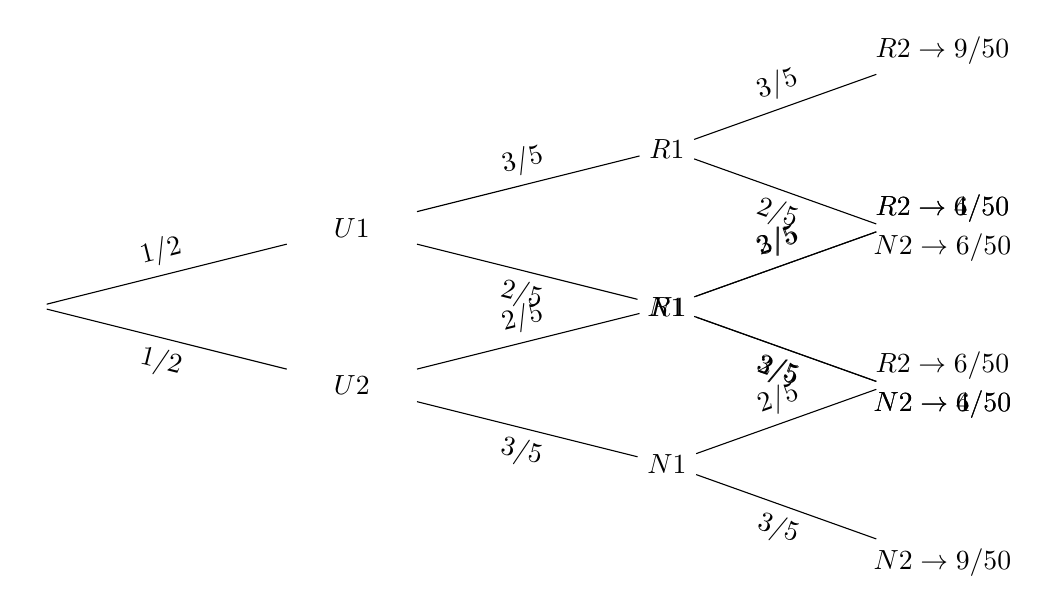
\begin{tikzpicture}[grow=right, sloped]
\node {}
    %******************************************************** RAMA 2
    child {
        node[bag] {$U2$}  
    %************************************************ RAMA 22
            child {
                node {$N1$}{}
            		child {
            		node {$N2 \to 9/50$}
            		edge from parent         
           			node[above] {}
            		node[below]  {$3/5$}
            		}
            		child {
            		node {$R2 \to 6/50$}
            		edge from parent         
           			node[above] {$2/5$}
            		node[below]  {}
            		}
            		edge from parent         
           			node[above] {}
            		node[below]  {$3/5$}
            }
    %************************************************ RAMA 21
            child {
                node {$R1$}{}
            		child {
            		node {$N2 \to 6/50$}
            		edge from parent         
           			node[above] {}
            		node[below]  {$3/5$}
            		}
            		child {
            		node {$R2 \to 4/50$}
            		edge from parent         
           			node[above] {$2/5$}
            		node[below]  {}
            		}
            		edge from parent         
           			node[above] {$2/5$}
            		node[below]  {}
            }
            edge from parent         
            node[above] {}
            node[below] {$1/2$}
    }
    %******************************************************** RAMA 1
    child {
        node[bag] {$U1$}   
    %************************************************ RAMA 12
            child {
                node {$N1$} {}
                	child {
            		node {$N2 \to 4/50$}
            		edge from parent         
           			 node[above] {}
            		 node[below]  {$2/5$}
            		}
            		child {
            		node {$R2 \to 6/50$ }
            		edge from parent         
           			node[above] {$3/5$}
            		node[below]  {}
            		}
            		 edge from parent         
           			 node[above] {}
            		 node[below]  {$2/5$}
            }
    %************************************************ RAMA 11
            child {
                node {$R1$} {}
               		child {
            		node {$N2 \to 6/50$}
            		edge from parent         
           			node[above] {}
            		node[below]  {$2/5$}
            		}
            		child {
            		node {$R2 \to 9/50$}
            		edge from parent         
           			node[above] {$3/5$}
            		node[below]  {}
            		}
            		edge from parent         
           			node[above] {$3/5$}
            		node[below]  {}
            } 
            edge from parent         
            node[above] {$1/2$}
            node[below]  {}
    }
    ;
\end{tikzpicture}


\vspace{20mm}%**********************************
$\Rightarrow  a)\quad  p(N1N2)=4/50+9/50=13/50=26\%$

\vspace{10mm}%*******
$\Rightarrow b)\quad p(\neq colores)=p(N1R2)+p(R1N2)=6/50+6/50+6/50+6/50=24/50=48\%$

\vspace{10mm}%*******
$\Rightarrow c)\quad p(N1|N2)=\dfrac{4/50+9/50}{6/50+4/50+6/50+9/50}=13/25=52\%$










\vspace{40mm} %*************************************************
\textcolor{blue}{B. Elegimos urna al azar y sacamos dos bolas sin reinserción.}


\vspace{20mm}%*******


% Set the overall layout of the tree
\tikzstyle{level 1}=[level distance=3.5cm, sibling distance=7cm]
\tikzstyle{level 2}=[level distance=3.5cm, sibling distance=3.5cm]
\tikzstyle{level 3}=[level distance=3.5cm, sibling distance=2cm]

% Define styles for bags and leafs
\tikzstyle{bag} = [text width=2em, text centered]
\tikzstyle{end} = [circle, minimum width=3pt,fill, inner sep=0pt]

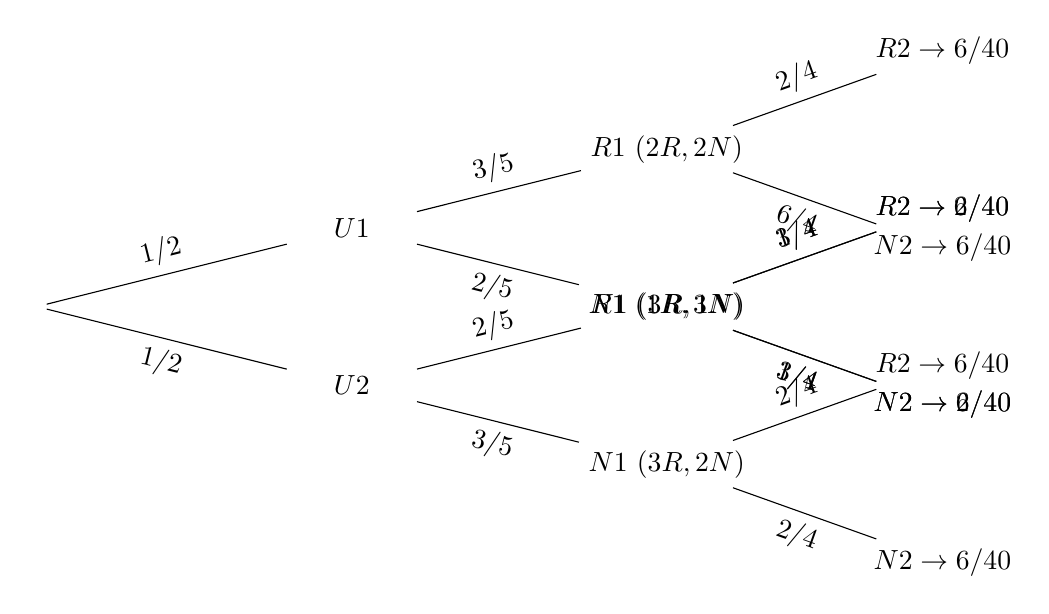
\begin{tikzpicture}[grow=right, sloped]
\node {}
    %******************************************************** RAMA 2
    child {
        node[bag] {$U2$}  
    %************************************************ RAMA 22
            child {
                node {$N1$ $(3R,2N)$}{}
            		child {
            		node {$N2 \to 6/40$}
            		edge from parent         
           			node[above] {}
            		node[below]  {$2/4$}
            		}
            		child {
            		node {$R2 \to 6/40$}
            		edge from parent         
           			node[above] {$2/4$}
            		node[below]  {}
            		}
            		edge from parent         
           			node[above] {}
            		node[below]  {$3/5$}
            }
    %************************************************ RAMA 21
            child {
                node {$R1$ $(1R,3N)$}{}
            		child {
            		node {$N2 \to 6/40$}
            		edge from parent         
           			node[above] {}
            		node[below]  {$3/4$}
            		}
            		child {
            		node {$R2 \to 2/40$}
            		edge from parent         
           			node[above] {$1/4$}
            		node[below]  {}
            		}
            		edge from parent         
           			node[above] {$2/5$}
            		node[below]  {}
            }
            edge from parent         
            node[above] {}
            node[below] {$1/2$}
    }
    %******************************************************** RAMA 1
    child {
        node[bag] {$U1$}   
    %************************************************ RAMA 12
            child {
                node {$N1$ $(3R,1N)$} {}
                	child {
            		node {$N2 \to 2/40$}
            		edge from parent         
           			 node[above] {}
            		 node[below]  {$1/4$}
            		}
            		child {
            		node {$R2 \to 6/40$ }
            		edge from parent         
           			node[above] {$3/4$}
            		node[below]  {}
            		}
            		 edge from parent         
           			 node[above] {}
            		 node[below]  {$2/5$}
            }
    %************************************************ RAMA 11
            child {
                node {$R1$ $(2R,2N)$} {}
               		child {
            		node {$N2 \to 6/40$}
            		edge from parent         
           			node[above] {}
            		node[below]  {$6/4$}
            		}
            		child {
            		node {$R2 \to 6/40$}
            		edge from parent         
           			node[above] {$2/4$}
            		node[below]  {}
            		}
            		edge from parent         
           			node[above] {$3/5$}
            		node[below]  {}
            } 
            edge from parent         
            node[above] {$1/2$}
            node[below]  {}
    }
    ;
\end{tikzpicture}


\vspace{20mm}%**********************************
$\Rightarrow  a)\quad  p(N1N2)=2/40+6/40=9/40=20\%$

\vspace{10mm}%*******
$\Rightarrow b)\quad p(\neq colores)=p(N1R2)+p(R1N2)=6/40+6/40+6/40+6/40=24/40=60\%$

\vspace{10mm}%*******
$\Rightarrow c)\quad p(N1|N2)=\dfrac{2/40+6/40}{6/40+2/40+6/40+6/40}=8/20=40\%$








\vspace{40mm}%********************************************* 
\textcolor{blue}{C. Sacamos una bola de cada urna (primero de la U1 y luego de la U2).}

\vspace{5mm} %*********************

% Set the overall layout of the tree
\tikzstyle{level 1}=[level distance=3.5cm, sibling distance=4cm]
\tikzstyle{level 2}=[level distance=3.5cm, sibling distance=2cm]

% Define styles for bags and leafs
\tikzstyle{bag} = [text width=4em, text centered]
\tikzstyle{end} = [circle, minimum width=3pt,fill, inner sep=0pt]

\begin{center}
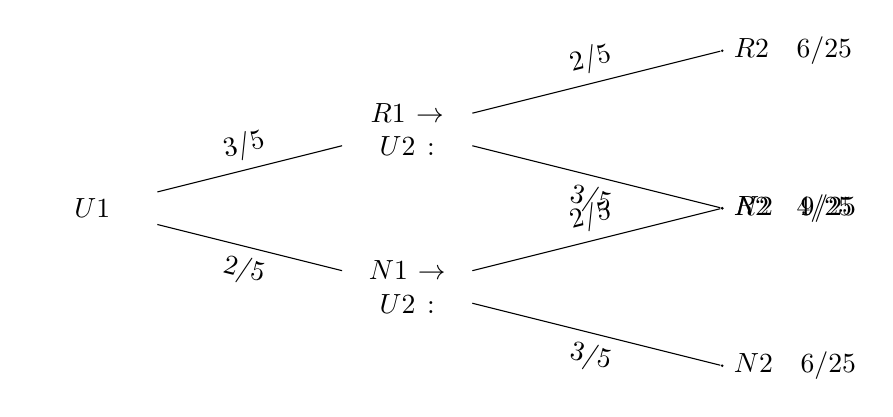
\begin{tikzpicture}[grow=right, sloped]
\node[bag] {$U1$}
    child {
        node[bag] {$\boldsymbol{N1} \to U2:$}        
            child {
                node[end, label=right: {$\boldsymbol{N2}\ \ \  6/25$}] {}
                edge from parent
                node[above] {}
                node[below]  {$3/5$}
            }
            child {
                node[end, label=right: {$\boldsymbol{R2}\quad 4/25$}] {}
                edge from parent
                node[above] {$2/5$}
                node[below]  {}
            }
            edge from parent 
            node[above] {}
            node[below]  {$2/5$}
    }
    child {
        node[bag] { {$\boldsymbol{R1} \to U2:$}}   
            child {
                node[end, label=right: {$\boldsymbol{N2}\quad 9/25$}] {}
                edge from parent
                node[above] {}
                node[below]  {$3/5$}
            }
            child {
                node[end, label=right: {$\boldsymbol{R2}\quad 6/25$}] {}
                edge from parent
                node[above] {$2/5$}
                node[below]  {}
            }
            edge from parent         
            node[above] {$3/5$}
            node[below]  {}
    };
\end{tikzpicture}
\end{center}

\vspace{5mm}%**********************************
$\Rightarrow  a)\quad  p(N1N2)=6/25=24\%$


$\Rightarrow b)\quad p(\neq colores)=p(N1R2)+p(R1N2)=9/25+4/25=52\%$


$\Rightarrow c)\quad p(N1|N2)=\dfrac{6/25}{9/25+6/25}=6/15=40\%$






\vspace{10mm} \textcolor{blue}{D. Trasvasamos una bola (R1 o N1) de la urna U1 a la urna U2 y extraemos bola (R2 o N2).}

\vspace{5mm}%**********************************

% Set the overall layout of the tree
\tikzstyle{level 1}=[level distance=3.5cm, sibling distance=4cm]
\tikzstyle{level 2}=[level distance=3.5cm, sibling distance=2cm]

% Define styles for bags and leafs
\tikzstyle{bag} = [text width=4em, text centered]
\tikzstyle{end} = [circle, minimum width=3pt,fill, inner sep=0pt]

\begin{center}
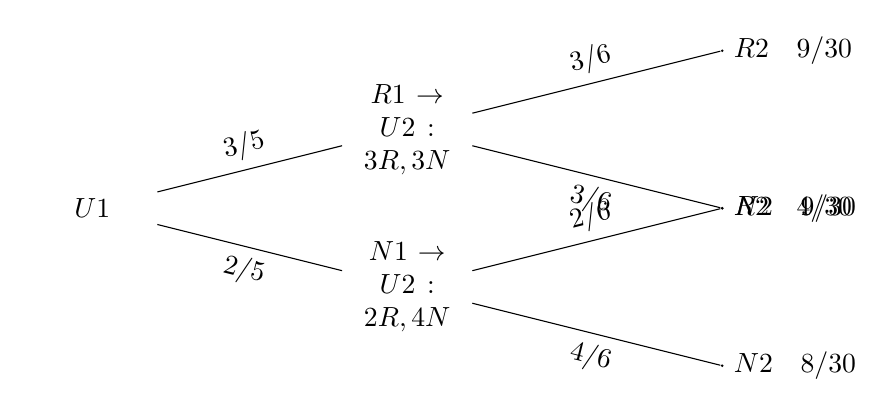
\begin{tikzpicture}[grow=right, sloped]
\node[bag] {$U1$}
    child {
        node[bag] {$\boldsymbol{N1} \to U2:$ $2R,4N$}        
            child {
                node[end, label=right: {$\boldsymbol{N2}\ \ \  8/30$}] {}
                edge from parent
                node[above] {}
                node[below]  {$4/6$}
            }
            child {
                node[end, label=right: {$\boldsymbol{R2}\quad 4/30$}] {}
                edge from parent
                node[above] {$2/6$}
                node[below]  {}
            }
            edge from parent 
            node[above] {}
            node[below]  {$2/5$}
    }
    child {
        node[bag] { {$\boldsymbol{R1} \to U2:$ $3R,3N$}}   
            child {
                node[end, label=right: {$\boldsymbol{N2}\quad 9/30$}] {}
                edge from parent
                node[above] {}
                node[below]  {$3/6$}
            }
            child {
                node[end, label=right: {$\boldsymbol{R2}\quad 9/30$}] {}
                edge from parent
                node[above] {$3/6$}
                node[below]  {}
            }
            edge from parent         
            node[above] {$3/5$}
            node[below]  {}
    };
\end{tikzpicture}
\end{center}

\vspace{5mm}%**********************************
$\Rightarrow  a)\quad  p(N1N2)=8/30=26.7\%$


$\Rightarrow b)\quad p(\neq colores)=p(N1R2)+p(R1N2)=4/30+9/30=13/30=43.3\%$


$\Rightarrow c)\quad p(N1|N2)=\dfrac{8/30}{9/30+8/30}=8/17=47.1\%$



\vspace{5mm}
\begin{ejemplo}
\begin{ejer}
De una baraja española de 40 cartas se extraen dos de ellas (sin reeemplazamiento). Calcula la probabilidad de que:

a) las dos sean reyes.

b) una sea de copas	y otra sea rey.

c) al menos una de ellas sea de copas.
\end{ejer}
\end{ejemplo}

Este problemas lo resolveremos razonando.

a) p(dos reyes)=p(1$^a$ rey y 2$^a$ rey)=$p(R1\cap R2)=p(R1)\cdot p(R2|R1)=\dfrac 4 {40}\cdot \dfrac 3{39}=0.77\%$

b) p(una de copas y otra rey)=p(1$^a$ copas y 2$^a$ rey) + p(1$^a$ rey y 2$^a$ copas)

Si hacemos $p(Co1 \cap R2)+p(R1\cap Co2)=p(co1)\cdot p(R2|Co1)+p(R1)\cdot p(Co2|R1)$

En $p(Co1 \cap R2)$ se nos presenta el siguiente problema: que la segunda rey si la primera es copas, $p(R2|Co1)$, es algo delicado, pues la primera podría haber sido ser el rey de copas, con lo que quedarían 3/39 y no 4/39 reyes en la baraja.

Cuando saquemos la carta de copas vamos a distinguir si esa carta es de copas excluido el rey de copas o si es el rey de copas: $p(Co)=p(Co-RCo)+p(RCo)$, así, 

$p(Co1 \cap R2)=p(Co-RCo1\cap R2)+p(RCo1\cap R2)=\dfrac 9 {40} \cdot \dfrac 4{39} + \dfrac{1}{40} \cdot \dfrac 3{39}$

Para el suceso $p(R1\cap Co2)$ estamos en las mismas, al sacar $R1$ puede que sea el rey de copas u otro, haremos $R1=RnoCo1 \ \cup RCo1$, distinguiremos así entre sacar un rey que no sea de copas (quedan 10/39 copas en la baraja) o sacar el rey de copas (quedan 9/39 copas en la baraja).

$p(R1 \cap Co2)=p(RnoCo1\cap Co2)+p(Rco1\cap Co2) =\dfrac{3}{40}\cdot \dfrac{10}{39} + \dfrac{1}{40}\cdot \dfrac{9}{39} =$

$=\dfrac{(9\cdot 4+1\cdot 3)+(3\cdot 10 + 1\cdot 9)}{40\cdot 39}=\dfrac{78}{1560}=5\%$

c) al menos una carta será de copas cuando lo sea la primera, o la segunda, o las dos. Es más sencillo pensar en el suceso contrario: `(al menos una es de copas)'$ \ '$=`ninguna es de copas'.

p(ninguna Co)=$p(noCo1 \cap noCo2)=p(noCo1)\cdot p(noCo2|noCo1)=\dfrac {30}{40}\cdot \dfrac {29}{39}=\dfrac{870}{1560}$

Por lo que p(al menos una es de Copas)=$1-\dfrac{870}{1560}=\dfrac{690}{1560}=44.2\%$

\vspace{5mm}
\begin{ejemplo}
\begin{ejer}
Un 65\% de los alumnos de un centro han aprobado Matemáticas, un 70\% ha aprobado Filosofía, y un 53\% ha aprobado ambas materias. Si se elige al azar un estudiante, calcúlese la probabilidad de que: 

a) haya aprobado al menos una de las dos materias.

b) haya suspendido ambas materias

c) Si aprobó Matemáticas ¿Cuál es la probabilidad de haber aprobado Filosofía? 	
\end{ejer}
\end{ejemplo}
Resolveremos este ejercicio mediante un diagrama de Venn. Trabajamos en tantos por cien.

	\begin{figure}[H]
				\centering
			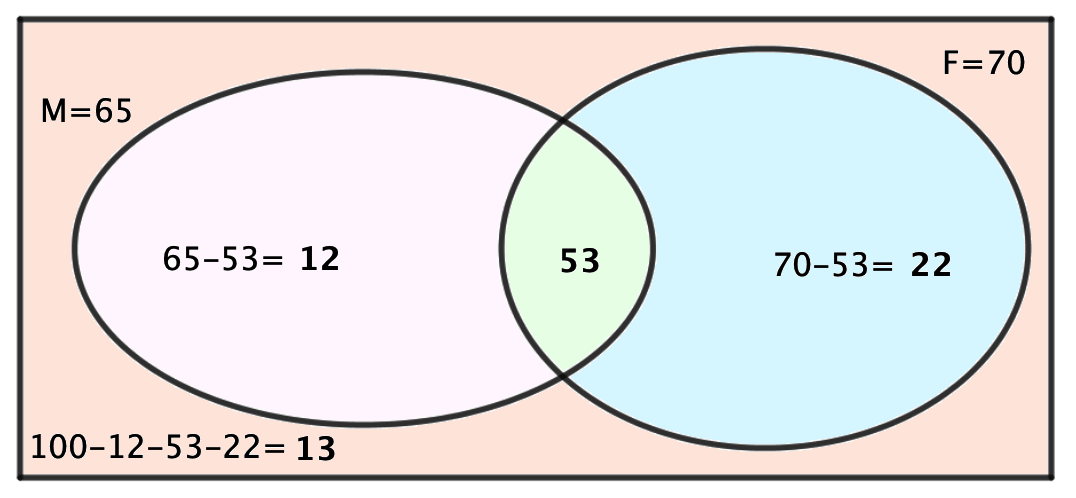
\includegraphics[width=.55\textwidth]{imagenes/imagenes02/T02IM29.png}
	\end{figure}

$a)\ p(\text{aprobar alguna})=p(M\cup F)=(12+53+22)\%=87\%$

$b)\ p(\text{suspender ambas})=p(M\cup F)'=p(M'\cap F')=1-87\%=13\%$

$c)\ p(F|M)=53/65\approx 81.5\%$

\textcolor{gris}{\rule{100mm}{0.1mm}}
\begin{multicols}{2}
\textcolor{gris}{Podría haberse intentado resolver el problema mediante una tabla de contingencia}

\begin{table}[H]
\centering
\begin{tabular}{c|c|c|c}
 & \textbf{F} & \textbf{F'} & \textbf{} \\ \hline
\multicolumn{1}{c|}{\textbf{M}} & 53 &  & 65 \\ \hline
\multicolumn{1}{c|}{\textbf{M'}} &  &  &  \\ \hline
\multicolumn{1}{c|}{\textbf{}} & 70 &  & \textbf{100}
\end{tabular}
\end{table}
\end{multicols}
\begin{flushright}
\vspace{-10mm}\textcolor{gris}{\rule{100mm}{0.1mm}}	
\end{flushright}

\vspace{5mm}
\begin{ejemplo}
\begin{ejer}\textcolor{white}{.}

\begin{multicols}{2}
Suponiendo que la riqueza es independiente del sexo, completar la siguiente tabla y calcular:

a)	probabilidad de que sabiendo que una persona no es pobre, sea hombre.

b) probabilidad de que una persona sea rica o mujer.

\begin{table}[H]
\centering
\begin{tabular}{c|c|c|c|}
\cline{2-4}
 & Rico & Pobre & Total \\ \hline
\multicolumn{1}{|c|}{Hombre} &  &  & 0.607 \\ \hline
\multicolumn{1}{|c|}{Mujer} &  &  & 0.393 \\ \hline
 & 0.002 &  &  \\ \cline{2-4} 
\end{tabular}
\end{table}
\end{multicols}
	
\end{ejer}
\end{ejemplo}
Tenemos una tabla de contingencia, las suma total debe ser \textcolor{red}{\textbf{1}}.

Empezamos por llamar $x=p(Rico\cap Hombre)$, al ser la riqueza independiente del sexo, tendremos que $p(Rico|Hombre)=x/0.607$ ha de coincidir con $p(Rico)=0.002$. De ahí: $x/0.607=0.002 \to$ \textcolor{red}{$\boldsymbol{x=0.0012}$}.

A partir de ahí, sin más que restar por filas, obtenemos $p(Pobre\cap Hombre)=0.607-0-0012=0.6058$

Obtenemos la $p(Pobre)$ sin más que restar en la columna final: $1-0.002=0.998$

Las dos probabilidades que faltan, se pueden obtener sin más que restar columnas. Con todo ellos, tenemos:

\begin{table}[H]
\centering
\begin{tabular}{c|c|c|c|}
\cline{2-4}
 & Rico & Pobre & Total \\ \hline
\multicolumn{1}{|c|}{Hombre} & \textcolor{red}{\textbf{x=0.0012}} & 0.6058 & \textbf{0.607} \\ \hline
\multicolumn{1}{|c|}{Mujer} & 0.0008 & 0.3922 & \textbf{0.393} \\ \hline
 & \textbf{0.002} & 0.998 & \textcolor{red}{\textbf{1}} \\ \cline{2-4} 
\end{tabular}
\end{table}

$a)\ \ p(Hombre|no\ Pobre)=p(Hombre|Rico)=0.0012/0.002=60\%$

$b)\ \ p(Rico \ o \ Hombre)=p(Rico\cup Homnre)=0.0008+0.0012+0.6058=0.6078$



\vspace{5mm}
\begin{ejemplo}
\begin{ejer}
La ciudad A tiene el doble de habitantes que la ciudad B, pero un 30\% de ciudadanos de B lee literatura, mientras que sólo un 10\% de ciudadanos da A lee literatura. 

a)  De un ciudadano se sabe sólo que vive en la ciudad A o en la ciudad B.  Calcula de forma razonada que lea literatura.

b)  Si nos presentan un ciudadano que vive en la ciudad A o en la ciudad B, pero del cual sabemos que lee literatura, calcula razonadamente la probabilidad de que sea de la ciudad B. 	
\end{ejer}
\end{ejemplo}
El problema es lo bastante sencillo como para resolverlo con cualquiera de las tres estrategias (árbol, Ven o tabla), tan solo hay que considerar que si en A hay doble población que B, sea x=población de B, luego 2x=población de A y 3x=población total. Con esto, p(A)=2/3 y p(B)=1/3.

	\begin{figure}[H]
				\centering
			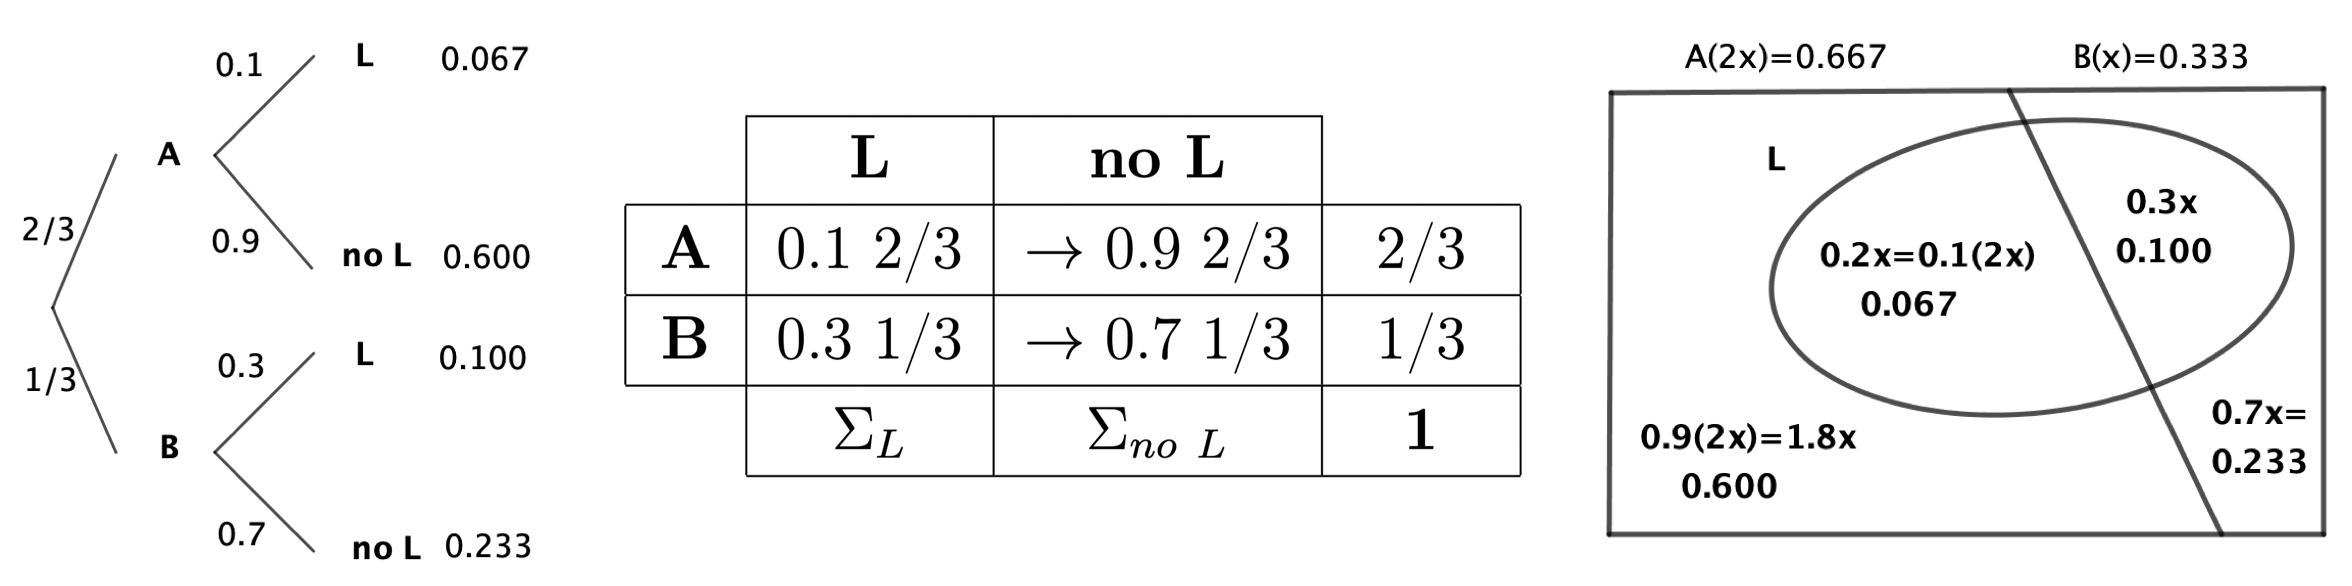
\includegraphics[width=1\textwidth]{imagenes/imagenes02/T02IM30.png}
	\end{figure}

$a)\ p(L)=0.067+0.100=0.167$

$b)\ p(A|L)=\dfrac{0.067}{0.067+0.100}=0.401$



\vspace{5mm}
\begin{ejemplo}
\begin{ejer}
Escribo tres cartas y los tres sobres correspondientes. Introduzco cada carta en un sobre al azar, es decir sin mirar el destinatario. Averiguar razonadamente cuál es la probabilidad de que haya introducido solo una carta en el sobre correcto.	
\end{ejer}
\end{ejemplo}
Resolveremos el problema por razonamiento. Si llamamos A,B,C a los sobres y a,b,c a las cartas, la situación ideal (acertarlos todos) sería  Aa,Bb,Cc.

\begin{multicols}{2}
Supongamos que tenemos los sobres ordenados, A,B,C y vamos a repartir las cartas al azar. Las distintas formas de ordenar 3 objetos a,b,c es 3!=6 (ver apéndice \ref{combinatoria} de Combinatoria, también es fácil de deducir mediante un esquema en árbol). Estos son los casos posibles.

Ahora veamos los casos favorables a acertar solo una carta con su sobre. Si se trata de la carta a, la solución sería Aa,Bc,Cb y no hay más. Solo hay, también, una sola forma de acertar la carta b (Ac, Bb, Ca) y una sola para la carta c (Ab,Ba,Cc). En total, 3 casos posibles.

Aplicando la regla de Laplace:  

\hspace{1cm} p(acertar solo una)=$\dfrac 3 6 =50\%$.

	\begin{figure}[H]
				\centering
			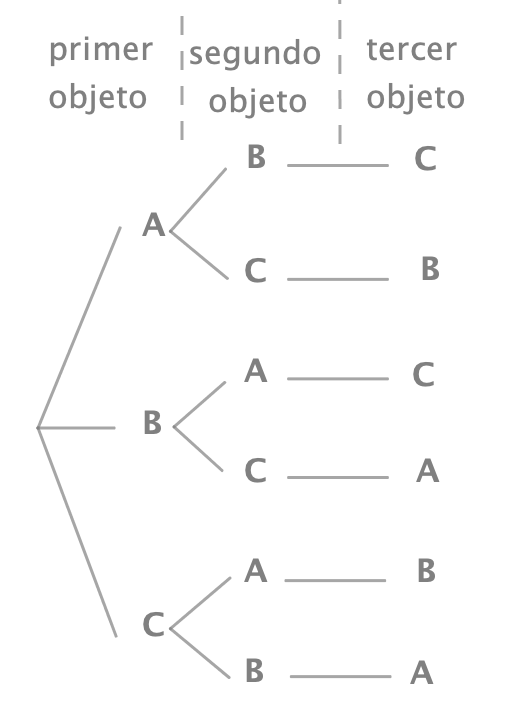
\includegraphics[width=.3\textwidth]{imagenes/imagenes02/T02IM31.png}
	\caption*{\footnotesize{Formas de ordenar 3 objetos}}
	\end{figure}	
\end{multicols}

\vspace{5mm}
\begin{ejemplo}
\begin{ejer}
En un curso de 40 alumnos hay 24 que aprueban Historia, 20 aprueban Lengua y 27 aprueban Filosofía. Sabiendo que no hay ninguno que las suspenda todas, ?`cuál es la probabilidad de que al elegir a un alumno al azar, haya aprobado la Historia y la Lengua?. Sabemos también que las tres asignaturas las aprueban 10 alumnos, que 14 aprueban Filosofía e Historia y que 15 aprueban Lengua y Filosofía.

Si sabemos que un alumno ha aprobado la Historia, ?`cuál es la probabilidad de que apruebe Lengua?

Los sucesos `aprobar Lengua' y `aprobar Historia', ?`son incompatibles?, ?`son independientes?. Razona tus respuestas.	
\end{ejer}
\end{ejemplo}
Usaremos un diagrama de Venn con tres conjuntos compatibles (que se intersecten entre ellos). Ojo a las intersecciones.

En este caso trabajaremos con números absolutos, dentro del rectángulo (referencial) han de estar los 40 alumnos. (Ver figura adjunta).

Empezamos colocando $10=H\cap L\cap F$. Como en todo $F\cap H=14$, fuera de la triple intersección colocaremos $14-10=4$. Lo mismo para $L\cap F$, esos 15 son los 10 de la triple intersección y 5 de fuera.

$L\cap H????$.  Llamaremos $x$ a los alumnos que han aprobado \underline{solo} F y H, excluyendo a los 10 que también han aprobado F, así en $F\cap H$ harán $10+x$.

Completamos ahora las zonas en que solo aparecen H, L o F. De este modo, en F hay 27-4-10-5=8; en H, 6-x, y en L, 5-x. Como hay 0 fuera de los tres conjuntos, ya tenemos a todo el alumnado colocado. Sumándolos a todos hemos de obtener 40 $\ \to x=2$
	\begin{figure}[H]
				\centering
			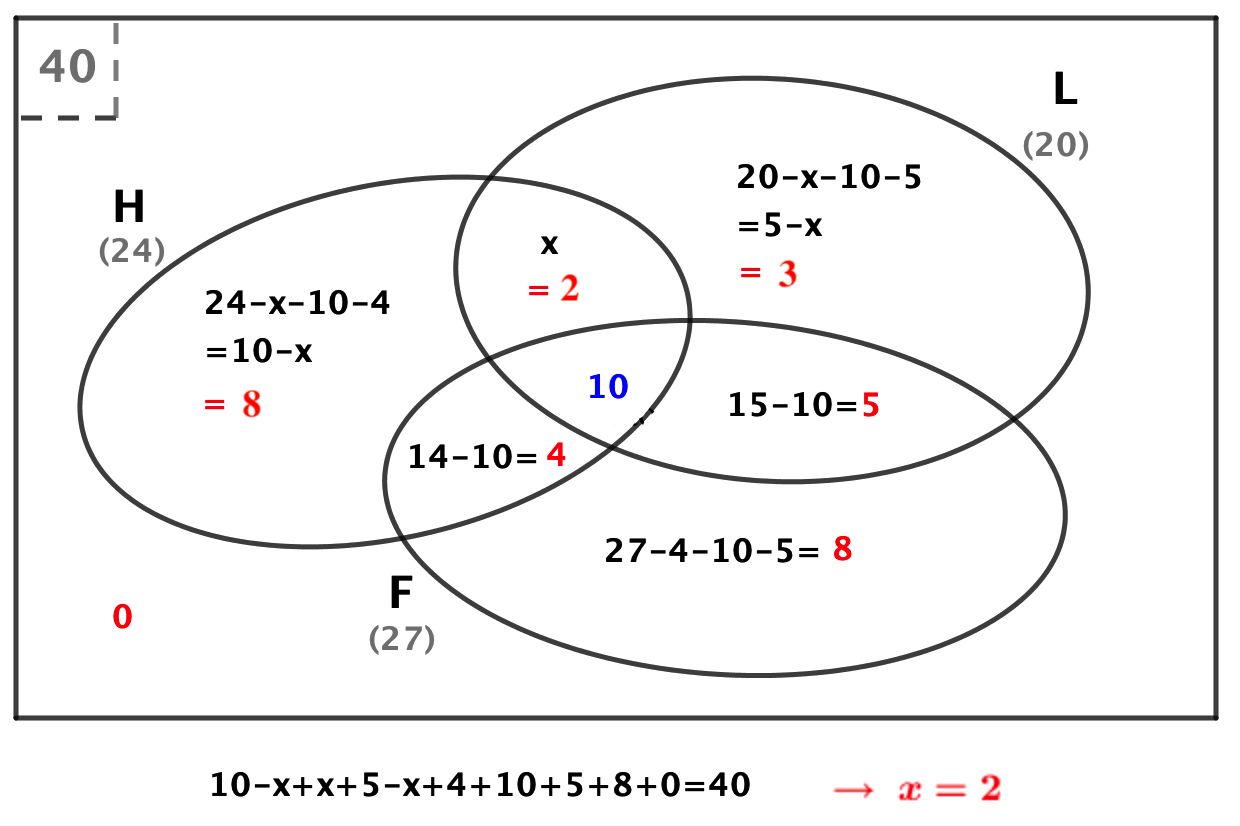
\includegraphics[width=.7\textwidth]{imagenes/imagenes02/T02IM32.png}
	\end{figure}
$p(H\cup L)=(8+2+3+4+10+5)/40=32/40=80\%$

$p(L|H)=(10+2)/(24)=50\%$

$p(L|H)=50\% = p(L)=20/40=50\% \ \to $, H y L son independientes.
\vspace{5mm}
\begin{ejemplo}
\begin{ejer}
En el palacio de rey Nebuzaradan hay 3 cámaras con dos cofres en cada una de ellas. En la primera cámara, cada cofre contiene un diamante, en la segunda hay una esmeralda dentro de cada cofre, y en la tercera, un cofre contiene un diamante y el otro una esmeralda. Un ladrón escoge una de las tres cámaras al azar y roba uno de los cofres. ?`Cuál es la probabilidad de que haya robado un diamante? Si cuando llega a su escondite descubre que ha robado una esmeralda, ?`cuál es la probabilidad de que dentro del segundo cofre de la misma cámara en que ha entrado hubiese un diamante?	
\end{ejer}
\end{ejemplo}
\begin{multicols}{2}
$\quad$

$p(D)=1/6+1/6+1/6=0.5$

$\quad$

$p(C3|D)=\dfrac{1/6}{1/6+1/6+1/6}=0.33$
	\begin{figure}[H]
				\centering
			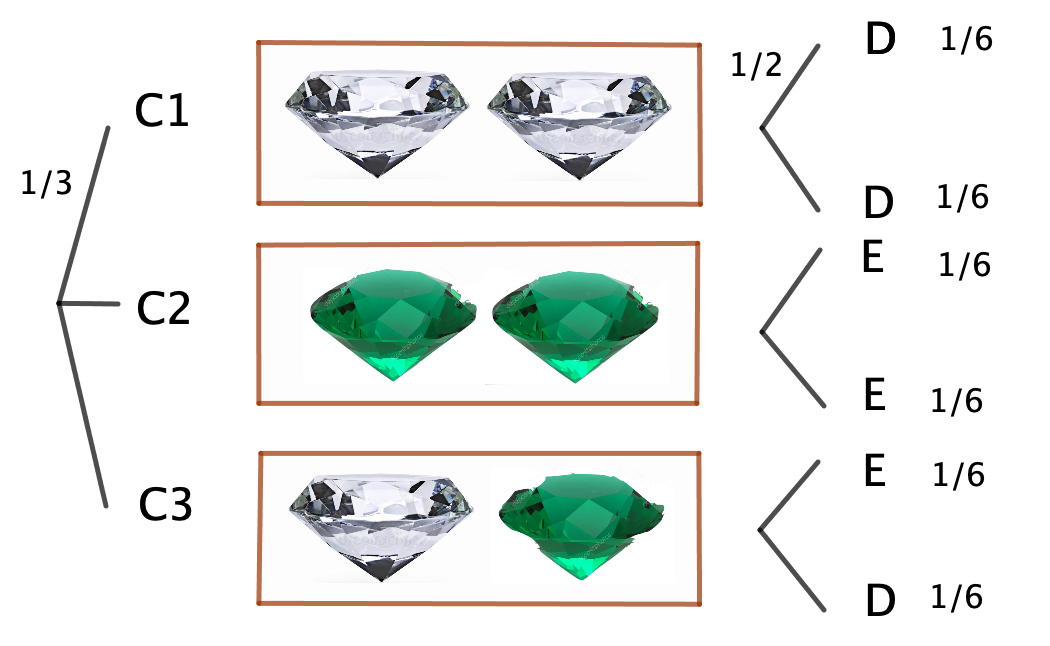
\includegraphics[width=.4\textwidth]{imagenes/imagenes02/T02IM33.png}
	\end{figure}	
\end{multicols}	


\vspace{5mm}
\begin{ejemplo}
\begin{ejer}\textcolor{white}{.}

En 1912, durante su primer viaje a través del Atlántico, el transatlántico Titanic chocó contra un iceberg y se hundió. En la siguiente tabla tienes información sobre el número de mujeres que sobrevivieron y murieron en relación a su nivel económico: 


\begin{table}[H]
\centering
\begin{tabular}{|c|r|r|}
\hline
\textbf{Nivel económico} & \multicolumn{1}{c|}{\textbf{Murieron}} & \multicolumn{1}{c|}{\textbf{Sobreviveron}} \\ \hline
\textbf{Alto}            & 6                                      & 126                                        \\ \hline
\textbf{Medio}           & 13                                     & 90                                         \\ \hline
\textbf{Bajo}            & 107                                    & 101                                        \\ \hline
\end{tabular}
\end{table}
 
 ?`Cuál es la probabilidad de que una mujer de nivel alto sobreviviera? ?`Y una de nivel medio? ?`Y una de nivel bajo? 

?`Cuál es la probabilidad de que una mujer que sobrevivió a la catástrofe fuera de nivel alto? ?`Y de nivel medio? ?`Y de nivel bajo? 
	
\end{ejer}
\end{ejemplo}
Primero, calculemos las sumas parciales:

\begin{table}[H]
\centering
\begin{tabular}{c|r|r|c}
\cline{1-3}
\multicolumn{1}{|c|}{\textbf{Nivel económico}} & \multicolumn{1}{c|}{\textbf{Murieron}} & \multicolumn{1}{c|}{\textbf{Sobreviveron}} & totales                 \\ \hline
\multicolumn{1}{|c|}{\textbf{Alto}}            & 6                                      & 126                                        & 132                     \\ \hline
\multicolumn{1}{|c|}{\textbf{Medio}}           & 13                                     & 90                                         & 103                     \\ \hline
\multicolumn{1}{|c|}{\textbf{Bajo}}            & 107                                    & 101                                        & 208                     \\ \hline
totales                                        & 126                                    & 317                                        & \multicolumn{1}{c}{443}
\end{tabular}
\end{table}

San A, M, B los sucesos `la persona elegida es de nivel económico alto', `medio', `bajo', y Mu, So los sucesos `la persona elegida murió', `sobrevivió´'.


\begin{table}[H]
\small
\centering
\begin{tabular}{lll}
$p(So|A)=126/132=95,5\%\ ;$ & $p(So|M)=90/103=87.4\%;\ $ & $p(So|B)=101/208=48.6\%$ \\ \\
$p(A|So)=126/317=39.7\%;\ $ & $p(M|So)=90/317=28.4;\ $ & $p(B|So)=101/317=31.9\%$
\end{tabular}
\end{table}



\vspace{5mm}
\begin{ejemplo}
\begin{ejer}
En una bolsa de caramelos surtidos hay 10 caramelos de sabor naranja (N), 5 sabor a limón (L) y 3 con sabor a fresa (F). Todos tienen el mismo tamaño y hasta extraerlos de la bolsa no se sabe de que sabor son. Se extraen tres caramelos al azar.

a) Calcular de forma razonada la probabilidad de extraer primero uno con sabor naranja, luego uno con sabor a fresa y, por último, uno con sabor a limón.

b) Calcular de forma razonada la probabilidad de que sean de tres sabores diferentes.	
\end{ejer}
\end{ejemplo}
Aunque el problema parece estar pidiendo ser abordado por un diagrama de árbol, necesitaríamos 3x3x3=27 hojas. Excesivo, así que lo intentamos resolver razonándolo. Cada caramelo, en cada una de las tres extracciones, lo denotaremos por $N_i,\ L_i,\ F_i$, donde con $i=1,2,3$ indicamos el orden en la extracción.

$a)\ p(N1\cap F2\cap L3)=p(N1)\cdot p(F2|L1) \cdot p(L3|N1\cap F2)=
\dfrac{10}{18}\cdot \dfrac{3}{17}\cdot \dfrac{5}{16}=\dfrac{10\cdot 3\cdot 5}{18\cdot 17\cdot 16}=\dfrac{150}{4896}\approx 3\%$

\begin{small}
\vspace{2mm}\textcolor{gris}{Sacar el primer caramelo de naranja tiene una probabilidad de 10/18. Quedan en la bolsa 17 caramelos (9N, 5L, 3F). Sacar ahora uno de fresa tiene una probabilidad de 3/17, quedando 16 caramelos en la bolsa (9N, 5L, 2F), por lo que la probabilidad de sacar esta vez uno de limón es de 5/16. En total, $(10\cdot 3 \cdot 5)(18\cdot 17 \cdot 16)\approx 3\%$.}
\end{small}

$b)\ p(\text{distintos sabores})$. Las distintas formas do ordenar 3 objetos son $3!=6$, todas ellas con las mismas probabilidades.

$\to p(\text{distintos sabores})=6\cdot p(NFL)=6\cdot \dfrac{150}{4896}\approx 18\%$

\begin{small}
\vspace{2mm}\textcolor{gris}{Hay que considerar ls siguientes casos de ordenar los tres sabores:}

\textcolor{gris}{--- NFL, con probabilidad $(10\cdot 3 \cdot 5)/(18\cdot 17 \cdot 16)$}

\textcolor{gris}{--- NLF, con probabilidad $(10\cdot 5 \cdot 3)/(18\cdot 17 \cdot 16)$}

\textcolor{gris}{--- FNL, con probabilidad $(3\cdot 10 \cdot 5)/(18\cdot 17 \cdot 16)$}

\textcolor{gris}{--- LNF, con probabilidad $(5\cdot 10 \cdot 3)/(18\cdot 17 \cdot 16)$}

\textcolor{gris}{--- LFN, con probabilidad $(5\cdot 3 \cdot 10)/(18\cdot 17 \cdot 16)$}

\textcolor{gris}{Todas los probabilidades son iguales (tanto numeradores como denominadores), luego:}

\textcolor{gris}{$\to p(\text{distintos sabores})=6\cdot p(NFL)=6\cdot \dfrac{150}{4896}\approx 18\%$}
\end{small}

\vspace{5mm}
\begin{ejemplo}
\begin{ejer}
Para elegir a un muchacho entre tres se prepara una bolsa con dos bolas negras y una bola blanca. Los tres van sacando, por orden, una bola que no devuelven. Quién saque la bola blanca gana. ?`Quién lleva más ventaja: el primero, el segundo o el tercero? 	
\end{ejer}
\end{ejemplo}
\begin{multicols}{2}
	\begin{figure}[H]
				\centering
			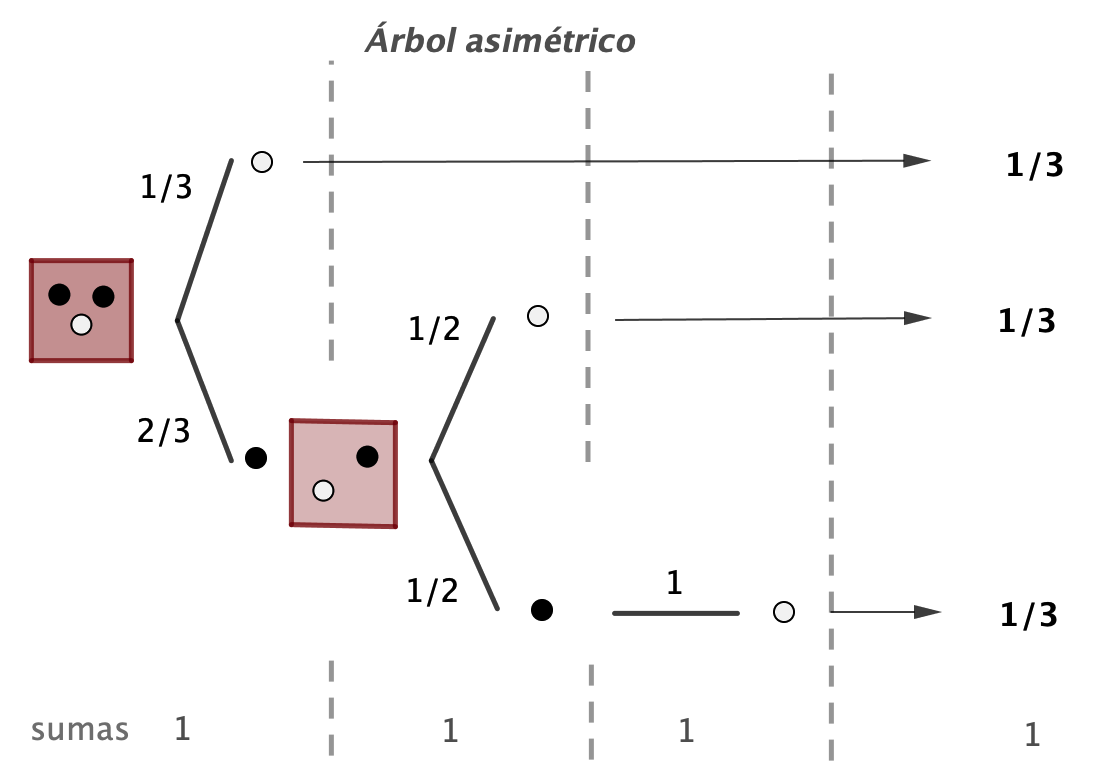
\includegraphics[width=.5\textwidth]{imagenes/imagenes02/T02IM34.png}
	\end{figure}
Cuando un jugador saca bola blanca, gana y acaba el juego (\emph{árbol asimétrico}).

Primer jugador, $p(Blanca)=1/3$

Segundo jugador, $p(Blanca)=2/3 \cdot 1/2=1/3$

Tercer jugador, $p(Blanca)=2/3 \cdot 1/2 \cdot 1=1/3$

Independientemente del turno de cada jugador, todos tienen la misma probabilidad de ganar.
\end{multicols}
\vspace{5mm}
\begin{ejemplo}

\begin{ejer}
Mr. Stoneguy, un experimentado comerciante de diamantes, decide recompensar a su hijo permitiéndole escoger una de dos cajas. Cada caja contiene 3 diamantes. En una de las cajas 2 de los diamantes son reales y el otro es una excelente imitación; en la otra caja uno es real y los otros dos son imitaciones. Si el hijo escoge aleatoriamente entre las dos cajas, su oportunidad de conseguir 2 diamantes verdaderos es 1/2, por lo que Mr. Stoneguy decide ayudarlo de la siguiente manera: permite a su hijo sacar un diamante de una de las cajas y examinarlo para ver si es un verdadero diamante; si el diamante examinado es real, el hijo se queda con esa caja, y se queda con la otra caja en el otro caso. ?`Cuál es la probabilidad de que el hijo se quede con 2 verdaderos diamantes. 	
\end{ejer}
\end{ejemplo}

El hijo de Mr. Stoneguy, primero elige caja (con probabilidades 1/2 para cada una de ellas) y, luego, saca un diamante. La probabilidad de que sea bueno es de 2/3 en la caja uno y de 1/3 en la dos. Si el diamante sacado es bueno, conserva la caja; si es malo, la cambia.

	\begin{figure}[H]
				\centering
			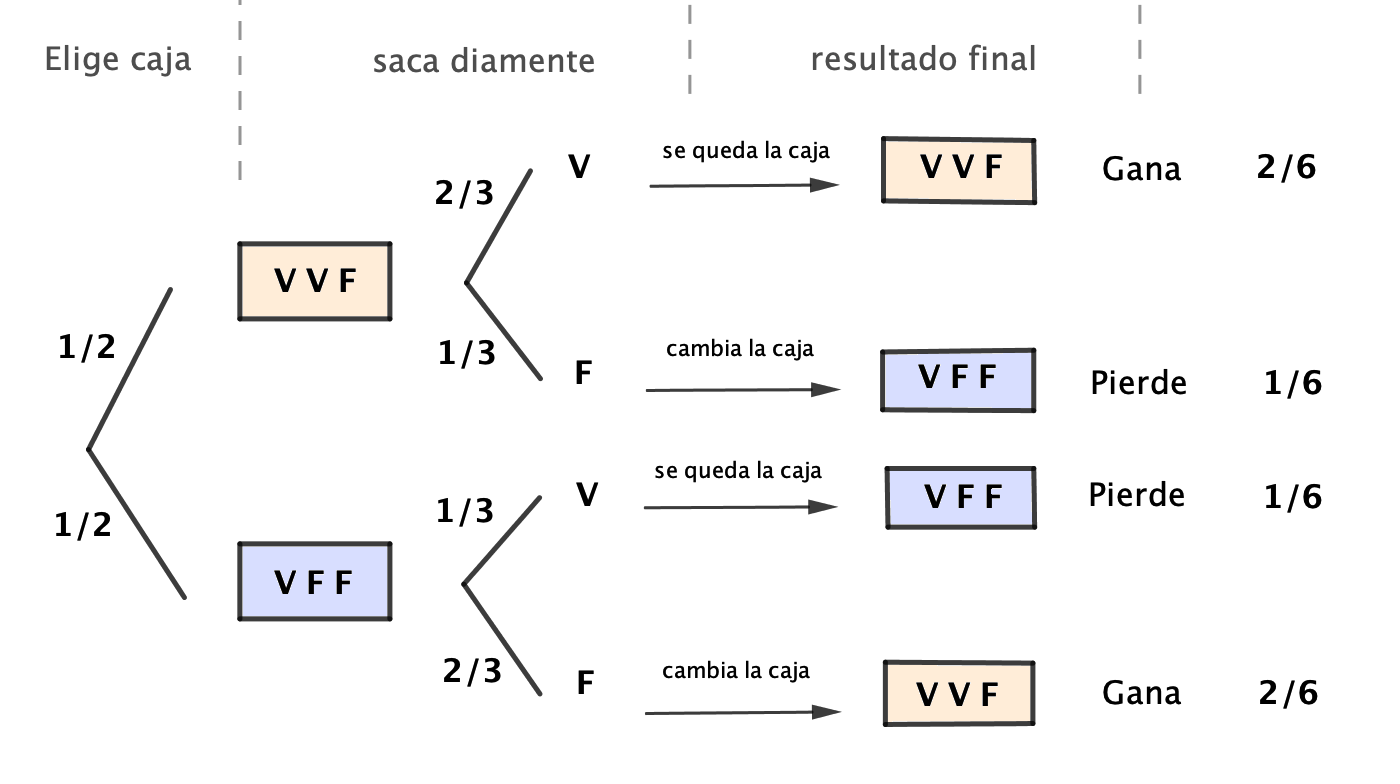
\includegraphics[width=.85\textwidth]{imagenes/imagenes02/T02IM35.png}
	\end{figure}

Decimos que el hijo `Gana' si, al final, se queda con la caja que contiene dos diamantes buenos, así:
$\ p(Gana)=2/6+2/6=66.7\%>50\%$, por lo que realmente Mr. Stoneguy sí ayuda a su hijo en la elección.

\vspace{5mm}
\begin{ejemplo}
\begin{ejer}
En un congreso de 200 jóvenes se pasa una encuesta para conocer los hábitos en cuanto a contratar viajes por internet. Se observa que de los encuestados, 120 son hombres de los que 84 de ellos contratan los viajes por internet., mientras que solo 24 de las mujeres lo hace.

Elegido un congresista al azar, calcula la probabilidad de que:

a) No contrate sus viajes por internet.

b) Sí use internet para contratar viajes , si la persona elegida es una mujer.

c) Sea un hombre, sabiendo que contrata sus viajes por internet.
\end{ejer}

\end{ejemplo}
El problema parece dispuesto para ser atacado por una tabla de contingencia. Pondremos en negrita los datos conocidos e iremos averiguando los que faltan (se han numerado en el orden en que se han averiguado) :

$a)\ \ p(No \ internet)=92/200; \quad$
$b)\ \ p(Internet | Mujer)=24/80; \quad$
$c)\ \ p(H | Internet)=84/108$

\begin{table}[H]
\centering
\begin{tabular}{c|c|c|c}
 & \textbf{\begin{tabular}[c]{@{}c@{}}Usa Internet\\ para los viajes\end{tabular}} & \textbf{\begin{tabular}[c]{@{}c@{}}No usa internet\\ para los viajes\end{tabular}} & \textbf{} \\ \hline
\textbf{Hombre} & \textbf{84} & \begin{tabular}[c]{@{}c@{}}(1)\\ 120-84 =\\ = 36\end{tabular} & \textbf{120} \\ \hline
\textbf{Mujer} & \textbf{24} & \begin{tabular}[c]{@{}c@{}}(3)\\ 80-24=\\ = 56\end{tabular} & \begin{tabular}[c]{@{}c@{}}(2)\\ 200-120=\\ = 80\end{tabular} \\ \hline
\textbf{} & \begin{tabular}[c]{@{}c@{}}(4)\\ 84+24=\\ = 108\end{tabular} & \begin{tabular}[c]{@{}c@{}}(4bis)\\ 36+56=\\ = 92\end{tabular} & \textbf{200}
\end{tabular}
\end{table}

\textcolor{gris}{\rule{70mm}{0.1mm}}	

Podría, con unos pocos cálculos (sobre todo para el árbol), abordarse el problema mediante un diagrama de Venn o mediante un diagrama de árbol.
	\begin{figure}[H]
				\centering
			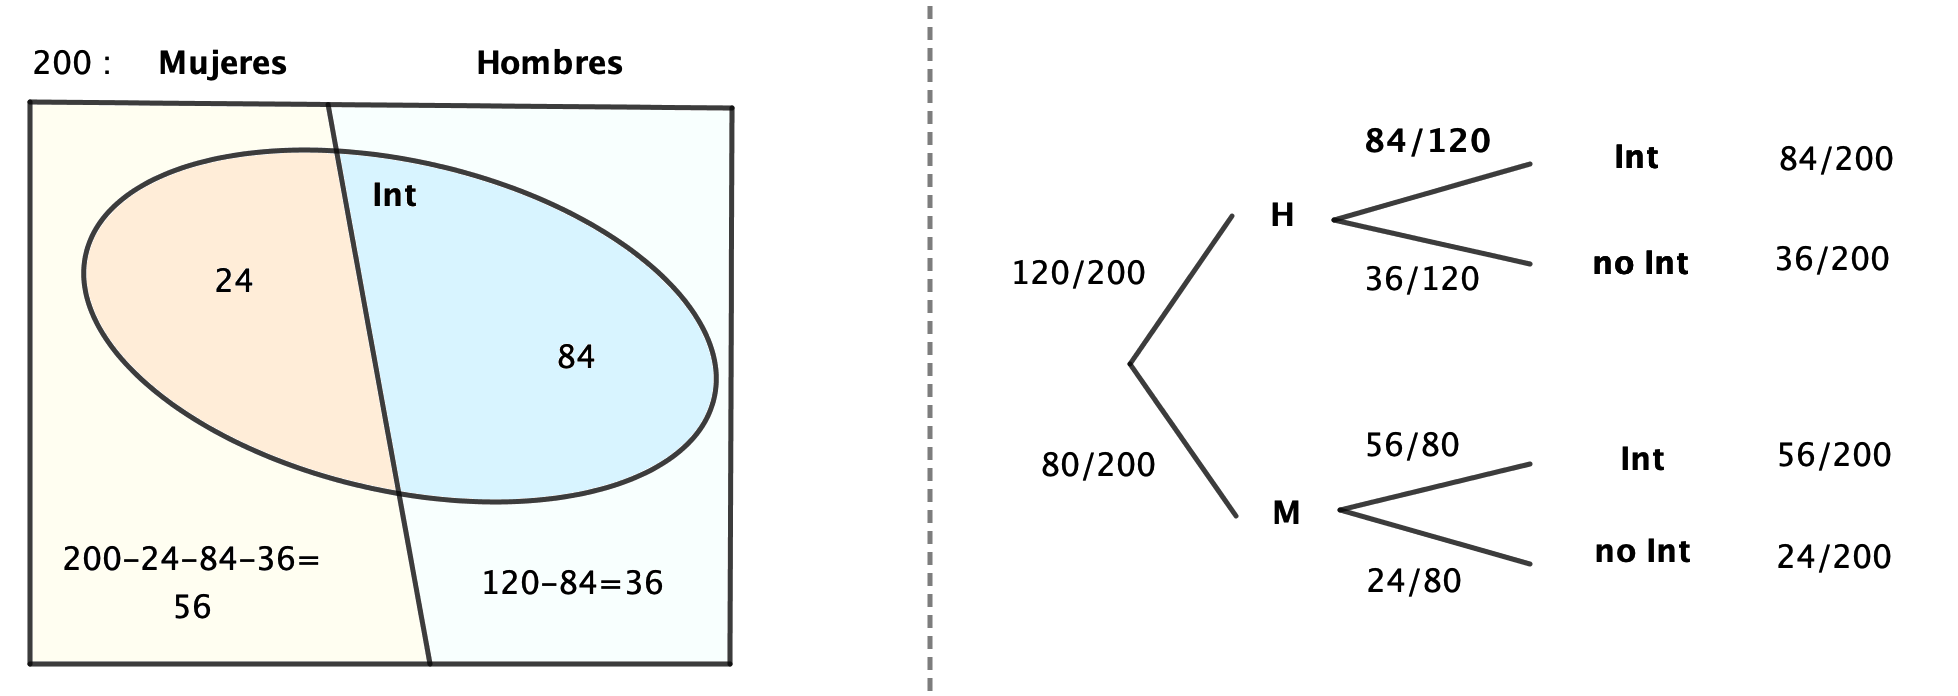
\includegraphics[width=1\textwidth]{imagenes/imagenes02/T02IM36.png}
	\end{figure}
\begin{flushright}
\vspace{-5mm}\textcolor{gris}{\rule{100mm}{0.1mm}}	
\end{flushright}



\vspace{5mm}
\begin{ejemplo}
\begin{ejer}
Se dispone de tres monedas. La primera de ellas es una moneda `cargada' de modo que la probabilidad de obtener cara es solo 0.4. La segunda moneda es una moneda `trucada' que tiene dos cruces y la tercera también está `cargada', pero de modo que la probabilidad de obtener cara es 0.6. Se pide:

a) Escribir el espacio muestral asociado al experimento aleatorio del lanzamiento ordenado de estas tres monedas.

b) Calcula la probabilidad de obtener exactamente dos cruces.

c) Calcula la probabilidad del suceso C1X2C3, es decir, cara en la primera moneda, crux en la segunda y cara en la tercera (CXC ordenadamente).

d) Calcula la probabilidad de obtener al menos una cara.
\end{ejer}
\end{ejemplo}
Abordamos el problema sin estrategia de árbol, Ven o contingencia, directamente.

Usamos la notación CXC para indicar que la primera moneda ha salido cara, C; la segunda cruz, X y la tercera cara. 

Para la primera moneda, p(C)=0.4 y p(X)=0.6. Para la segunda, p(C)=0 y p(X)=1. Para la tercera, p(C)=0.6 y p(X)=0.4.

$a)\ E=\{C\boldsymbol{X}C,\ C\boldsymbol{X}X,\ X\boldsymbol{X}C,\ X\boldsymbol{X}X\}$, la moneda central `trucada' siempre sale $\boldsymbol{X}$.

$b) \ $Observando el espacio muestral anterior y teniendo en cuenta las probabilidades para cada moneda,

$p(dos \ cruces)=p(CXX)+p(XXC)=0.4\cdot 1 \cdot 0.4+ 0.6\cdot 1 \cdot 0.6=0.16+0.36=0.52$

$c)\ p(CXC)=0.4\cdot 1 \cdot 0.6=0.24$

$d)\ $ El suceso contrario a `al menos una cara' es `todas cruz', así:

$p(\text{al menos una cara})=1-p(\text{todoa cruz})=1-p(XXX)=1-0.6\cdot 1 \cdot 0.4=1-0.24=0.78$


\vspace{3mm}
\begin{ejemplo}
\begin{ejer}
Un dado está cargado de modo que la probabilidad de obtener las distintas caras es proporcional al cuadrado del número que estas tienen.

?`Cuál es la probabilidad de obtener un 5? ?`Cuál es la probabilidad de obtener suma 7 en dos lanzamientos?	
\end{ejer}
\end{ejemplo}
\begin{small}
$p(1)=k;\ p(2)=k2^2=4k;\ p(3)=k3^2=9k;\ p(4)=k4^2=16k; \ p(5)=k5^2=25k;\ p(6)=k6^2=36k$ \end{small}

Como $\ \displaystyle \sum_{i=1}^6p(i)=1 \ \to \ k+4k+9k+16k+25k+36k=91k=1 \ \to k=1/91$

La probabilidad de obtener un 5 es: $p(5)=25k=25/91$

Para ver las probabilidades de las distintas sumas al lanzar dos dados podríamos construir una tabla de doble entrada, que va a ser largo, o usar el razonamiento.

Al lanzar dos dados se obtiene suma siete si salen (1,6), con la misma probabilidad que (6,1); o si sale (2,5) o (5,2); o si sale (3,4) o (4,3), así:

$p(suma\ 7)=2\cdot p(1,6)+ 2\cdot p(2,5)+2\cdot p(3,4)=
2\cdot \frac{1}{91}\frac{36}{91}+2\cdot \frac{4}{91} \frac{25}{91}+2\cdot \frac{9}{91} \frac{16}{91}= \dfrac{560}{8281}$

\vspace{3mm}
\begin{ejemplo}
\begin{ejer}
En un centro de secundaria, aprueban Biología 4 de cada 5 alumnos, las Matemáticas las aprueban 2 de cada 3 alumnos y 3 de cada 5 alumnos aprueban Lengua. Elegido al azar un alumno matriculado de esas asignaturas en ese centro, calcula la probabilidad de que a) Suspenda esas tres asignaturas, b) Suspenda solo una de ellas y c) los sucesos `aprobar biología' y `aprobar Matemáticas', ?`son independientes?.	
\end{ejer}
\end{ejemplo}

\vspace{-3mm} Llamaremos B, M, L a los sucesos aprobar Biología, Matemáticas y Lengua. llamaremos B', M' y L' a los sucesos suspender esas asignaturas.
Resolvemos el problema mediante un diagrama de árbol. (Presentamos, ahora, toda la información en él).

% Set the overall layout of the tree
\tikzstyle{level 1}=[level distance=1.5cm, sibling distance=10cm]
\tikzstyle{level 2}=[level distance=3.5cm, sibling distance=5cm]
\tikzstyle{level 3}=[level distance=6 cm, sibling distance=4cm]

% Define styles for bags and leafs
\tikzstyle{bag} = [text width=2em, text centered]
\tikzstyle{end} = [circle, minimum width=3pt,fill, inner sep=0pt]

%Define probabilidades en naranja con rectángulo negro de bordes redondeados
\tikzstyle{aristas}=[rectangle, rounded corners=2pt, fill=orange!20, draw=black, font=\small]

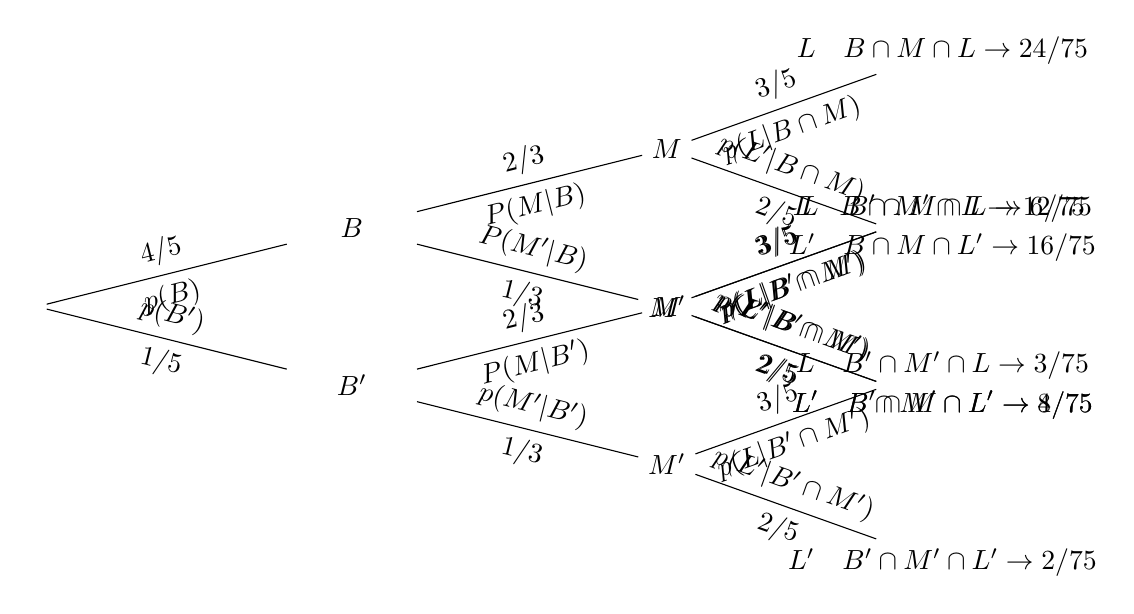
\begin{tikzpicture}[grow=right, sloped]
\node {}
    %******************************************************** RAMA 2
    child {
        node[bag] {$B'$}  
    %************************************************ RAMA 22
            child {
                node {$M'$}{}
            		child {
            		node {$L'\quad B'\cap M'\cap L' \to 2/75$}
            		edge from parent         
           			node[above] {$p(L'|B'\cap M')$}
            		node[below]  {$2/5$}
            		}
            		child {
            		node {$L\quad B'\cap M'\cap L \to 3/75$}
            		edge from parent         
           			node[above] {$3/5$}
            		node[below]  {$p(L|B'\cap M')$}
            		}
            		edge from parent         
           			node[above] {$p(M'|B')$}
            		node[below]  {$1/3$}
            }
    %************************************************ RAMA 21
            child {
                node {$M$}{}
            		child {
            		node {$L'\quad B'\cap M\cap L' \to 4/75$}
            		edge from parent         
           			node[above] {$p(L'|B'\cap M)$}
            		node[below]  {$2/5$}
            		}
            		child {
            		node {$L\quad B'\cap M\cap L \to 6/75$}
            		edge from parent         
           			node[above] {$3/5$}
            		node[below]  {$p(L|B'\cap M)$}
            		}
            		edge from parent         
           			node[above] {$2/3$}
            		node[below]  {$P(M|B')$}
            }
            edge from parent         
            node[above] {$p(B')$}
            node[below] {$1/5$}
    }
    %******************************************************** RAMA 1
    child {
        node[bag] {$B$}   
    %************************************************ RAMA 12
            child {
                node {$M'$} {}
                	child {
            		node {$L'\quad B\cap M'\cap L' \to 8/75$}
            		edge from parent         
           			 node[above] {$p(L'|B\cap M')$}
            		 node[below]  {$2/5$}
            		}
            		child {
            		node {$L\quad B\cap M'\cap L \to 12/75$}
            		edge from parent         
           			node[above] {$3/5$}
            		node[below]  {$p(L|B\cap M')$}
            		}
            		 edge from parent         
           			 node[above] {$P(M'|B)$}
            		 node[below]  {$1/3$}
            }
    %************************************************ RAMA 11
            child {
                node {$M$} {}
               		child {
            		node {$L'\quad B\cap M\cap L' \to 16/75$}
            		edge from parent         
           			node[above] {$p(L'|B \cap M)$}
            		node[below]  {$2/5$}
            		}
            		child {
            		node {$L\quad B\cap M\cap L \to 24/75$}
            		edge from parent         
           			node[above] {$3/5$}
            		node[below]  {$p(L|B\cap M)$}
            		}
            		edge from parent         
           			node[above] {$2/3$}
            		node[below]  {$P(M|B)$}
            } 
            edge from parent         
            node[above] {$4/5$}
            node[below]  {$p(B)$}
    }
    ;
\end{tikzpicture}

$a)\ \ p(\text{suspender las tres})=p(B'\cap M'\cap L')=2/75$

$b)\ \ p(\text{suspender solo una})=P(B'\cap M\cap L)+p(B\cap M'\cap L)+p(B\cap M \cap L')=$

$=6/75+12/75+16/75=34/75$


\vspace{5mm}
\begin{ejemplo}
\begin{ejer}
Un estudio revela que el 10\% de los oyentes de radio sintoniza a diario las cadenas Music y Rhythm, que un 35\% sintoniza a diario Music y que el 55\% de los oyentes no escucha ninguna de las dos emisoras . Obtén:

a) La probabilidad de que un oyente elegido al azar sintonice la cadena Rhythm.

b) La probabilidad de que un oyente elegido al azar sintonice la cadena Rhythm pero no la Music.

c) La probabilidad de que un oyente, del que sabemos que escucha Rhythm, escuche Music.	
\end{ejer}
\end{ejemplo}
Usaremos, para la resolución, un diagrama de Venn.

Llamamos R y M a los sucesos `la persona escucha Rhytm' y `la persona escucha Music', respectivamente.

	\begin{figure}[H]
		\centering
		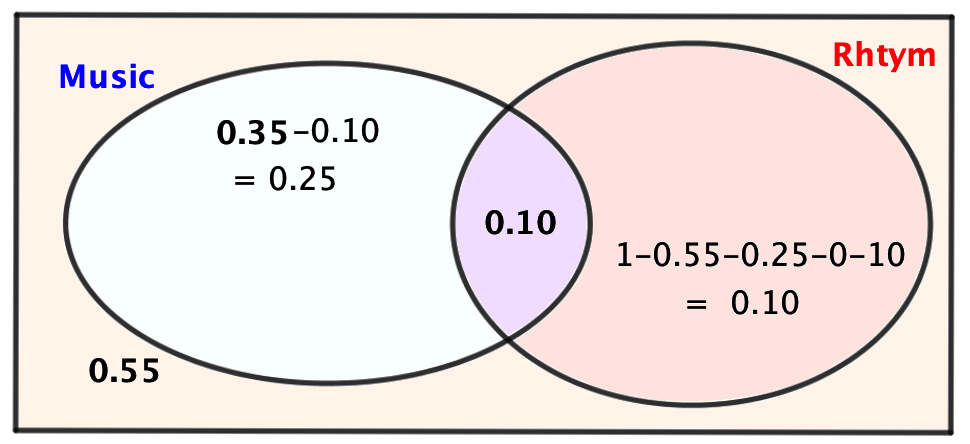
\includegraphics[width=.6\textwidth]{imagenes/imagenes02/T02IM37.png}
	\end{figure}
\vspace{-4mm} %**************************************
	
$a)\ \ p(R)=0.10+0.10=0.20$

$b)\ \ p(R-M)=0.10$

$c)\ \ p(M|R)=0.10/(0.10+0.10)=0.50$	
	
		
\vspace{5mm}
\begin{ejemplo}
\begin{ejer}
A un alumno le lleva en coche a la facultad el 80\% de las veces un amigo. Cuando le lleva en coche llega tarde el 20\% de los días. Cuando el amigo no le lleva, el alumno llega temprano a clase el 10\% de los días. Determinar:

a)  La probabilidad de que llegue pronto a clase y le haya llevado el amigo.

b)  La probabilidad de que llegue tarde a clase.

c)  Ha llegado pronto a clase. ?`Cuál es la probabilidad de que no le haya llevado su amigo?

d)  Llegar pronto a clase e ir en coche, ?`son sucesos independientes?.	
\end{ejer}
\end{ejemplo}
% Set the overall layout of the tree
\tikzstyle{level 1}=[level distance=4cm, sibling distance=2cm]
\tikzstyle{level 2}=[level distance=4cm, sibling distance=1.5cm]

% Define styles for bags and leafs
%\tikzstyle{bag} = [text width=6em, text centered]
%\tikzstyle{end} = [circle, minimum width=1pt,fill, inner sep=0pt]

%Define probabilidades en naranja con rectángulo negro de bordes redondeados
\tikzstyle{aristas}=[rectangle, rounded corners=2pt, fill=orange!20, draw=black, font=\small]

\begin{center}
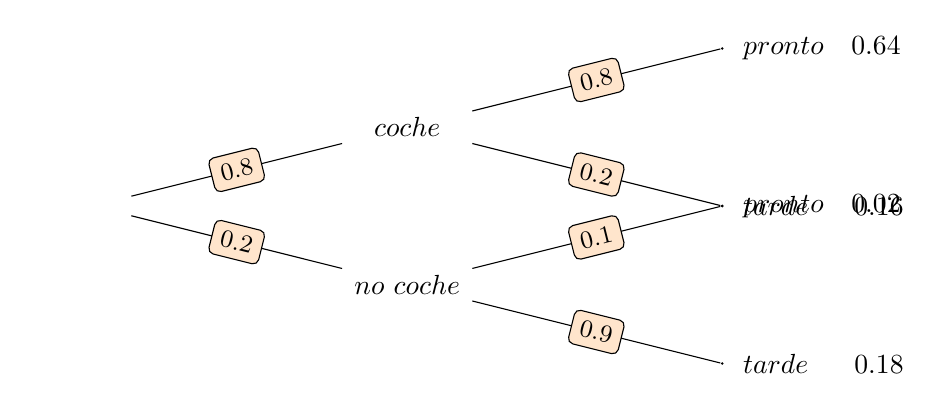
\begin{tikzpicture}[grow=right, sloped]
\node[bag] {}
    child {
        node[bag] {$\boldsymbol{no\ coche}$}        
            child {
                node[end, label=right: {$\ \boldsymbol{tarde}\quad \ \ 0.18$}] {}
                edge from parent
                node[aristas]  {$0.9$}
            }
            child {
                node[end, label=right: {$\ \boldsymbol{pronto}\quad 0.02$}] {}
                edge from parent
                node[aristas] {$0.1$}
            }
            edge from parent 
            node[aristas]  {$0.2$}
    }
    child {
        node[bag] {$\boldsymbol{coche}$}   
            child {
                node[end, label=right: {$\ \boldsymbol{tarde}\quad \ \ 0.16$}] {}
                edge from parent
                node[aristas]  {$0.2$}
            }
            child {
                node[end, label=right: {$\ \boldsymbol{pronto}\quad 0.64$}] {}
                edge from parent
                node[aristas] {$0.8$}
            }
            edge from parent         
            node[aristas] {$0.8$}
    };
\end{tikzpicture}
\end{center}

$a)\ p(pronto\ \cap \ coche)=0.64$

$b)\ p((tarde)=0.16+0.18=0.34$

$c)\ p(no \ coche\ | \ pronto)= 0.02/(0.64+0.02)\approx 0.03$

$d)\ p(no \ coche)=0.2 \neq 0.03 = p(no \ coche|pronto) \to$ los sucesos `coche' (o `no coche') y `pronto' no son independientes.

\vspace{5mm}
\begin{ejemplo}
\begin{ejer}
El 1\% de la población de un determinado lugar padece una enfermedad. Para detectar esta enfermedad se realiza una prueba de diagnóstico. Esta prueba da positiva en el 97\% de los pacientes que padecen la enfermedad; en el 98\% de los individuos que no la padecen da negativa. Si elegimos al azar un individuo de esa población:

a) ?`Cuál es la probabilidad de que el individuo dé positivo y padezca la enfermedad?
b) Si sabemos que ha dado positiva, ?`cuál es la probabilidad de que padezca la enfermedad?	
\end{ejer}
\end{ejemplo}

% Set the overall layout of the tree
\tikzstyle{level 1}=[level distance=4cm, sibling distance=3cm]
\tikzstyle{level 2}=[level distance=4cm, sibling distance=1.5cm]

% Define styles for bags and leafs
%\tikzstyle{bag} = [text width=4em, text centered]
%\tikzstyle{end} = [circle, minimum width=1pt,fill, inner sep=0pt]
%Define probabilidades en naranja con rectángulo negro de bordes redondeados
\tikzstyle{aristas}=[rectangle, rounded corners=2pt, fill=orange!20, draw=black, font=\small]

\begin{center}
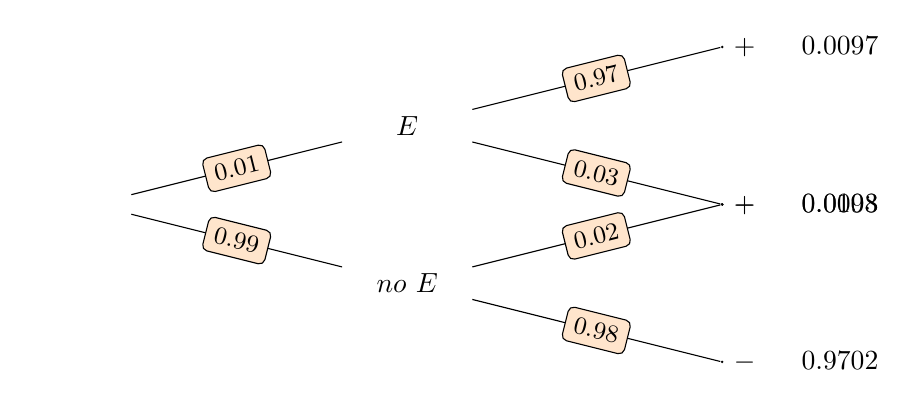
\begin{tikzpicture}[grow=right, sloped]
\node[bag] {}
    child {
        node[bag] {$\boldsymbol{no\ E}$}        
            child {
                node[end, label=right: {$\boldsymbol{-}\quad \ \ 0.9702$}] {}
                edge from parent
                node[aristas]  {$0.98$}
            }
            child {
                node[end, label=right: {$\boldsymbol{+}\quad \ \ 0.0198$}] {}
                edge from parent
                node[aristas] {$0.02$}
            }
            edge from parent 
            node[aristas]  {$0.99$}
    }
    child {
        node[bag] {$\boldsymbol{E}$}   
            child {
                node[end, label=right: {$\boldsymbol{-}\quad \ \ 0.0003$}] {}
                edge from parent
                node[aristas]  {$0.03$}
            }
            child {
                node[end, label=right: {$\boldsymbol{+}\quad \ \ 0.0097$}] {}
                edge from parent
                node[aristas] {$0.97$}
            }
            edge from parent         
            node[aristas] {$0.01$}
    };
\end{tikzpicture}
\end{center}

$a)\ \ p(E \cap +)=0.0097;\qquad b)\ \ p(E|+)=0.0097/(0.0097+0.0198)=32.9\%$

\vspace{5mm}
\begin{ejemplo}
\begin{ejer}
En cierto país, los ascensos de barrendero a jefe de escoba (JE) son  muy disputados. Se puede acceder por tres conductos: por oposición, por concurso de méritos o por enchufe con el ministro de Limpieza Pública.

La probabilidad de que un opositor alcance la plaza es de $0.2$. La probabilidad de que se obtenga la plaza si se concurso es $0,8$. Todos los enchufados del ministro de Limpieza Pública consiguen puesto.
Sabiendo que los aspirantes a jefes de escoba se reparten del siguiente modo: 70\% son opositores; 25\% concursan; 5\% consiguen el enchufe, calcular cuál es la probabilidad de que un cierto jefe de escoba alcance la plaza por oposición.	
\end{ejer}
\end{ejemplo}

\begin{center}
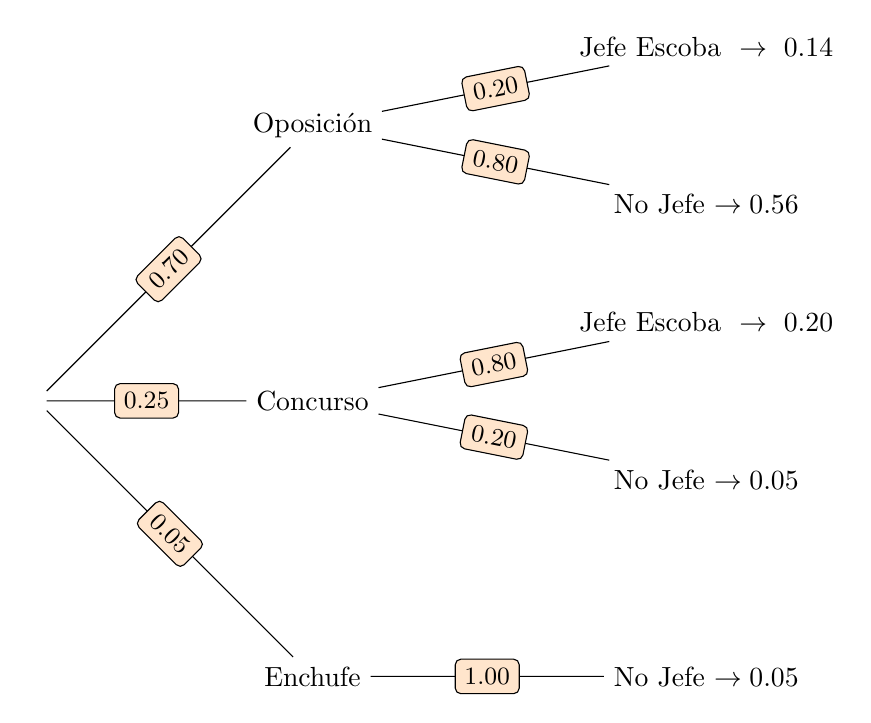
\begin{tikzpicture}[grow=right, sloped]

% Set the overall layout of the tree
\tikzstyle{level 1}=[level distance=3.5cm, sibling distance=3.5cm]
\tikzstyle{level 2}=[level distance=5cm, sibling distance=2cm]


% Define styles for bags and leafs
\tikzstyle{bag} = [text width=1em, text centered]
\tikzstyle{end} = [circle, minimum width=1pt,fill, inner sep=0pt]

%Define probabilidades en naranja con rectángulo negro de bordes redondeados
\tikzstyle{aristas}=[rectangle, rounded corners=2pt, fill=orange!20, draw=black, font=\small]

\node{}
	child{
    	node{Enchufe}
    	child{
    		node{No Jefe $\to 0.05$}
    		edge from parent
    		node[aristas]{$1.00$}
    		}
    	edge from parent
    	node[aristas]{$0.05$}
    }
    child{
    	node{Concurso}
    		child{
    		node{No Jefe $\to 0.05$}
    		edge from parent
    		node[aristas]{$0.20$}
    		}
    		child{
    		node{Jefe Escoba $\ \to \ 0.20$}
    		edge from parent
    		node[aristas]{$0.80$}
    		}
    	edge from parent
    	node[aristas]{$0.25$}
    }
    child{
    	node{Oposición}
    		child{
    		node{No Jefe $\to 0.56$}
    		edge from parent
    		node[aristas]{$0.80$}
    		}
    		child{
    		node{Jefe Escoba $\ \to \ 0.14$}
    		edge from parent
    		node[aristas]{$0.20$}
    		}
    	edge from parent
    	node[aristas]{$0.70$}
    }
	;
\end{tikzpicture}

$p(\text{Jefe Escoba}|\text{oposición})=\dfrac{0.14}{0.14+0.20+0.05} \approx 36 \%$
\end{center}


\vspace{5mm}
\begin{ejemplo}
\begin{ejer}
Un hombre y una mujer de la misma edad se casan a los 20 años. Las probabilidades de que lleguen a los 70 años son 0.76 para el hombre y 0.82 para la mujer.

Se pregunta cuál es la probabilidad de que a los 70 años:
\begin{adjustwidth}{20pt}{2pt}
	\begin{enumerate}[a) ]
	\item Ambos estén vivos
	\item No viva ninguno.
	\item Viva solamente la mujer.
	\item Viva al menos uno de los dos.	
	\end{enumerate}
\end{adjustwidth}
\end{ejer}
\end{ejemplo}

Podemos resolver el problema con un árbol o con una tabla.


\begin{multicols}{2}
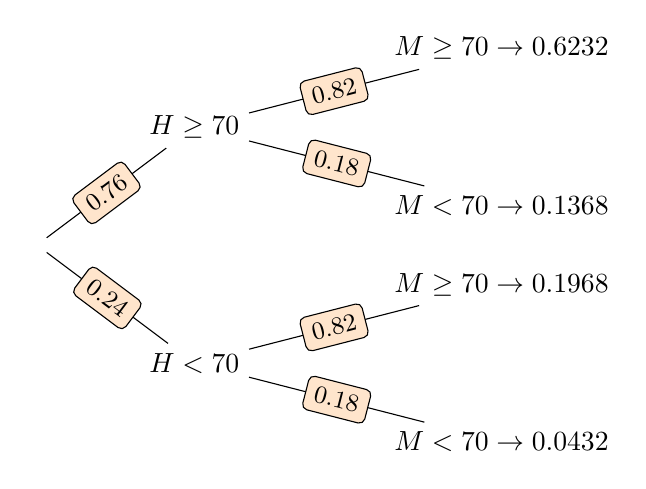
\begin{tikzpicture}[grow=right, sloped]

% Set the overall layout of the tree
\tikzstyle{level 1}=[level distance=2cm, sibling distance=3cm]
\tikzstyle{level 2}=[level distance=3.9cm, sibling distance=2cm]


% Define styles for bags and leafs
\tikzstyle{bag} = [text width=4em, text centered]
\tikzstyle{end} = [circle, minimum width=1pt,fill, inner sep=0pt]

%Define probabilidades en naranja con rectángulo negro de bordes redondeados
\tikzstyle{aristas}=[rectangle, rounded corners=2pt, fill=orange!20, draw=black, font=\small]

\node{}
    child{
    	node{$H<70$}
    		child{
    		node{$M<70 \to 0.0432$}
    		edge from parent
    		node[aristas]{$0.18$}
    		}
    		child{
    		node{$M\ge 70 \to 0.1968$}
    		edge from parent
    		node[aristas]{$0.82$}
    		}
    	edge from parent
    	node[aristas]{$0.24$}
    }
    child{
    	node{$H\ge 70$}
    		child{
    		node{$M<70 \to 0.1368$}
    		edge from parent
    		node[aristas]{$0.18$}
    		}
    		child{
    		node{$M\ge 70 \to 0.6232$}
    		edge from parent
    		node[aristas]{$0.82$}
    		}
    	edge from parent
    	node[aristas]{$0.76$}
    }
	;
\end{tikzpicture}

Hemos llamado $H\ge 70$ y $H<70$ a que el hombre llegue vivo a lo 70 años y de que no. Anlalogamente, para la mujer, $M\ge 70$ y $M<70$.


\begin{table}[H]
\centering
\begin{tabular}{c|c|c|c}
\cline{2-3}
\textbf{} & \textbf{$H\ge 70$} & \textbf{$H<70$} & \textbf{} \\ \hline
\multicolumn{1}{|c|}{\textbf{$M\ge 70$}} & 0.6232 & 0.1968 & \multicolumn{1}{c|}{\textbf{0.82}} \\ \hline
\multicolumn{1}{|c|}{\textbf{$M<70$}} & 0.1368 & 0.0432 & \multicolumn{1}{c|}{\textbf{0.18}} \\ \hline
\textbf{} & \textbf{0.76} & \textbf{0.24} & \textbf{} \\ \cline{2-3}
\end{tabular}
\end{table}
\end{multicols}

\begin{multicols}{2}
$p(\text{ambos vivos})=0.6232$

$p(\text{ninguno vivo})=0.0432$

$p(\text{solo vive mujer})=0.1968$

$p(\text{almenos uno vivo})=1-0.0432=0.9568$	
\end{multicols}


\vspace{5mm}
\begin{ejemplo}
\begin{ejer}
Se lanza una moneda y si sale cara se ponen 7 bolas blancas en una urna y si sale cruz se ponen 4 blancas. Se vuelve a lanzar la moneda y se ponen 5 o 2 bolas negras, según se saque cara o cruz. Después se saca una bola de urna así compuesta. ¿Cuál es la probabilidad de que la bola extraída sea negra? Si la bola ha sido negra, ¿cuál es la probabilidad de que hayan salido 2 veces cara? 	
\end{ejer}
\end{ejemplo}
	\begin{figure}[H]
		\centering
		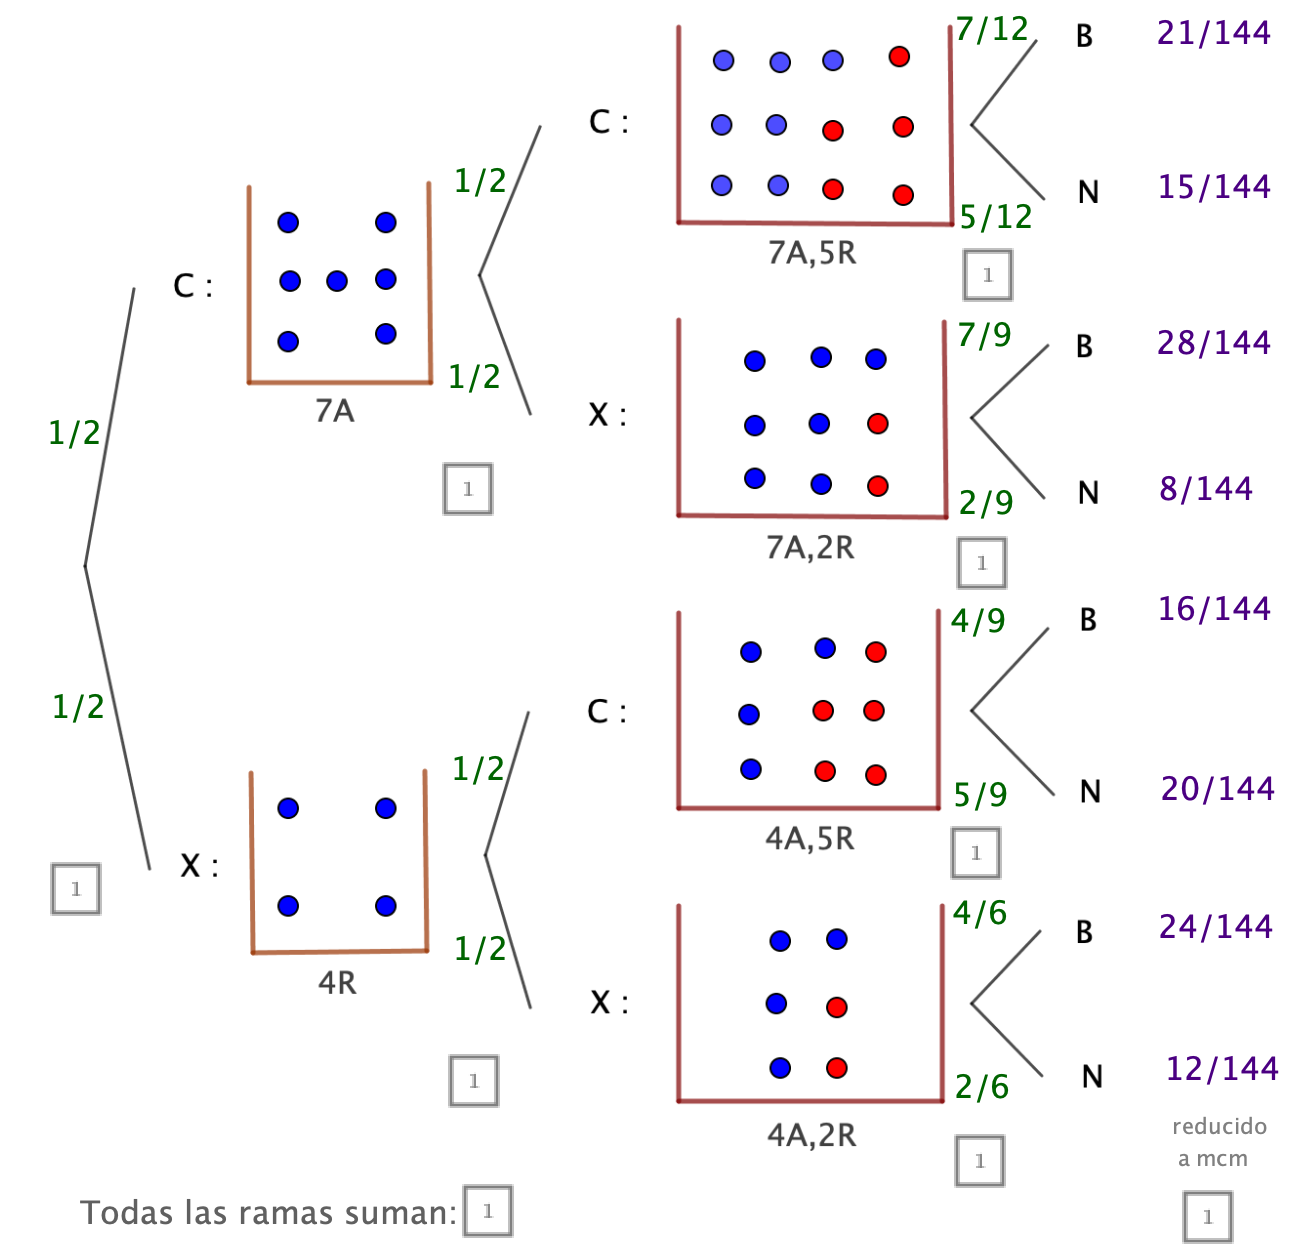
\includegraphics[width=1\textwidth]{imagenes/imagenes02/T02IM44.png}
	\end{figure}
	
$p(N)=15/144+8/144+20/144+12/144=55/144=38.2\%$

$p(C1\cap C2|N)=21/55=38.2\%$


\vspace{5mm}
\begin{ejemplo}
\begin{ejer}
Mr. Bandit, un bien conocido ranchero pero no bien conocido ladrón de ganado, tiene 20 cabezas de ganado listas para vender. Dieciséis de estas cabezas son suyas y consecuentemente llevan su propia marca. Las otras cuatro llevan marcas ajenas. Mr.Bandit sabe que el inspector de marcas revisa el 20\% del ganado de cualquier cargamento. Él tiene dos camiones, uno de los cuales puede cargar a las 20 cabezas a la vez, y el otro puede cargar sólo 10 cabezas. Mr. Bandit considera 4 estrategias en su intento de llevar el ganado al mercado para venderlo sin que sea descubierto: 1) enviar en un solo cargamento las 20 cabezas, 2) enviar dos cargamentos de 10 cabezas cada uno, en donde las 4 cabezas robadas se encuentran en uno de los viajes, 3) se envían dos cargamentos de 10, uno con 3 cabezas robadas y el otro con una, y 4) se envían dos cargamentos de 10, cada uno con dos cabezas robadas. ¿Qué estrategia minimiza la probabilidad de que Mr.Bandit sea descubierto?.	
\end{ejer}
\end{ejemplo}
	\begin{figure}[H]
		\centering
		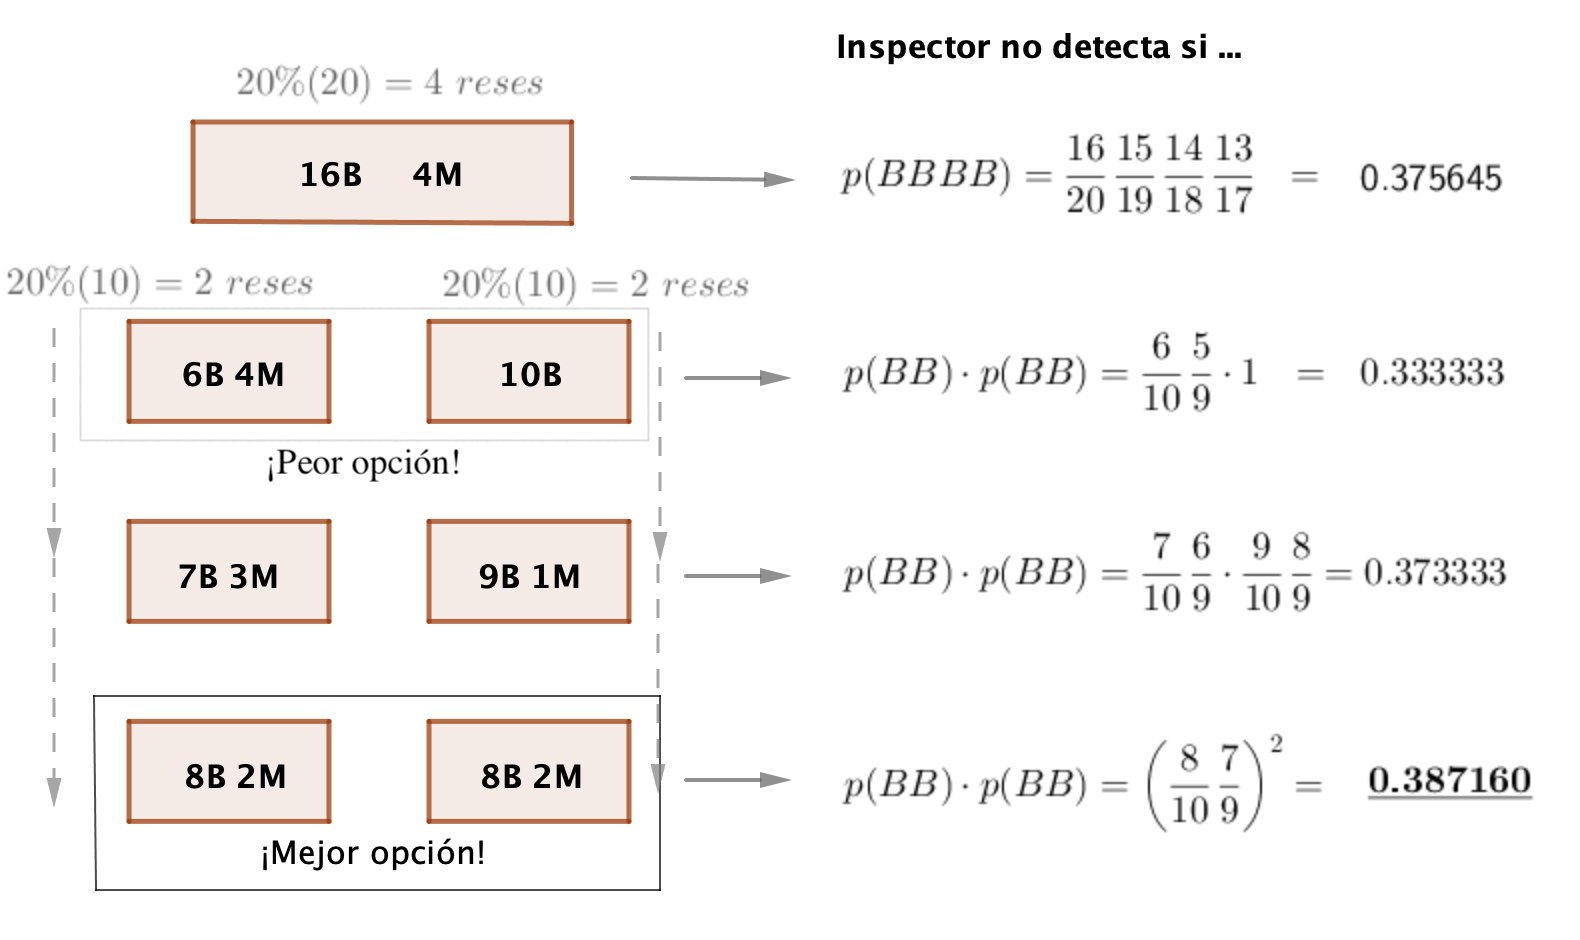
\includegraphics[width=1\textwidth]{imagenes/imagenes02/T02IM45.png}
	\end{figure}



\vspace{5mm}
\begin{ejemplo}
\begin{ejer}
Dispones de dos bolas rojas y dos bolas negras que disponer en dos urnas, con la condición de que nunca quede una urna sin bolas.

a) Comprueba que solo hay 4 disposiciones posibles.

b) En cada disposición posible de las 4 bolas en las dos urnas, te diriges a  ellas y extraes una bola de cada urna. ?`Cuál es la probabilidad, en cada disposición, de extraer bolas de distinto color?

c) ?`En qué disposición es mayor esta probabilidad? ?`Y menor?
\end{ejer}
\end{ejemplo}

	\begin{figure}[H]
		\centering
		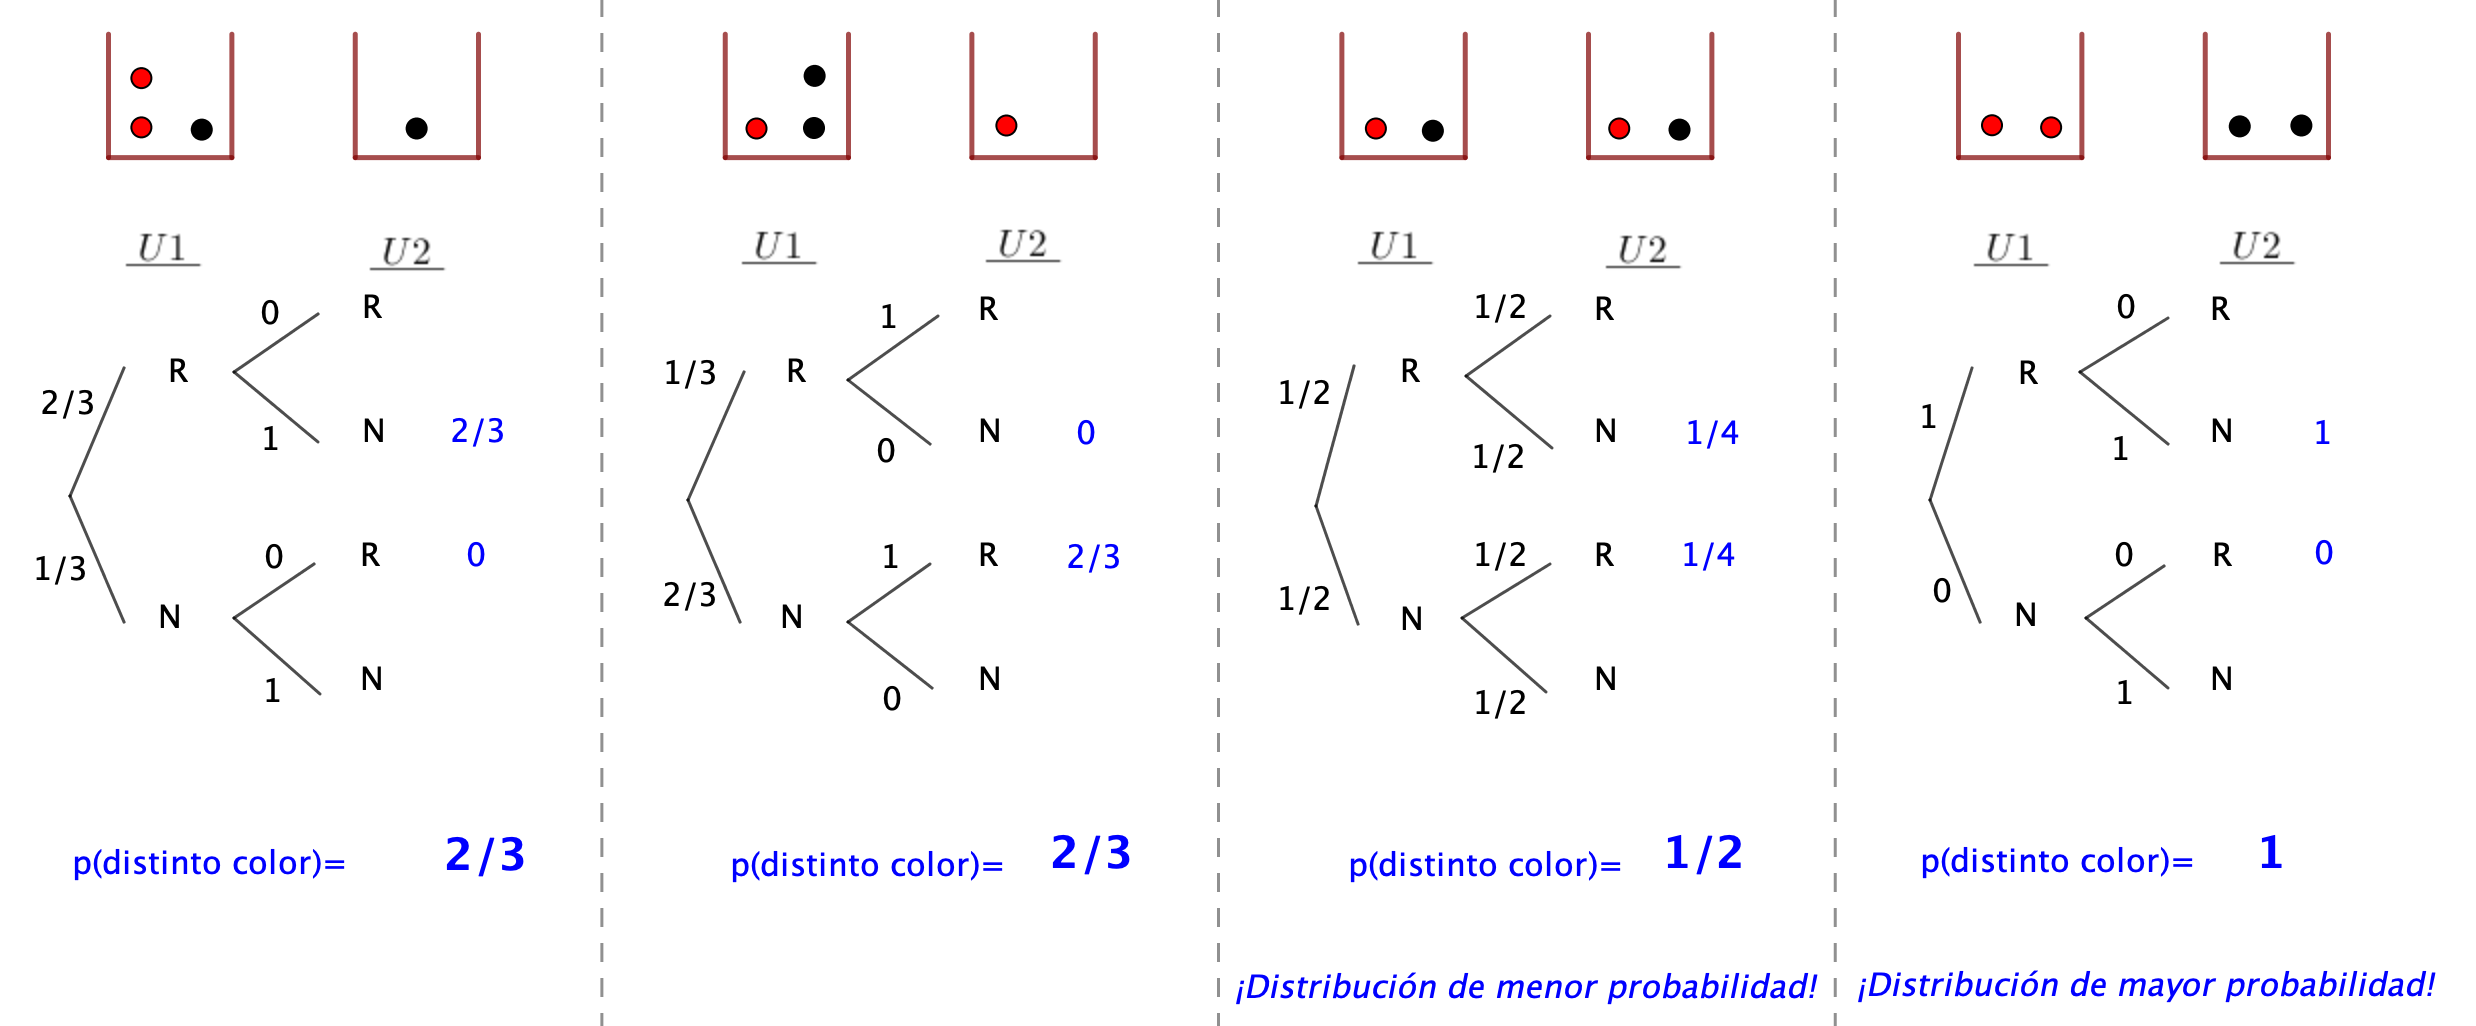
\includegraphics[width=1.05\textwidth]{imagenes/imagenes02/T02IM46.png}
	\end{figure}



\vspace{5mm}
\begin{ejemplo}
\begin{ejer}
En la figura se muestra un tiro al blanco. El punto central del tiro al blanco se llama diana. Se sabe que una persona da al tablero $9$ de cada $10$ veces que lanza y que, si ha dado al tablero, da a la diana proporcionalmente a la superficie de esta. Sabiendo que $R = 4r$, determine las siguientes probabilidades: 

P (corona); P (diana | tablero); P (tablero | corona); P (corona | no tablero); P (no tablero | diana) ; P (diana); P (tablero | diana); P (diana | no tablero); P (no tablero | corona); P (corona | tablero)

	\begin{figure}[H]
		\centering
		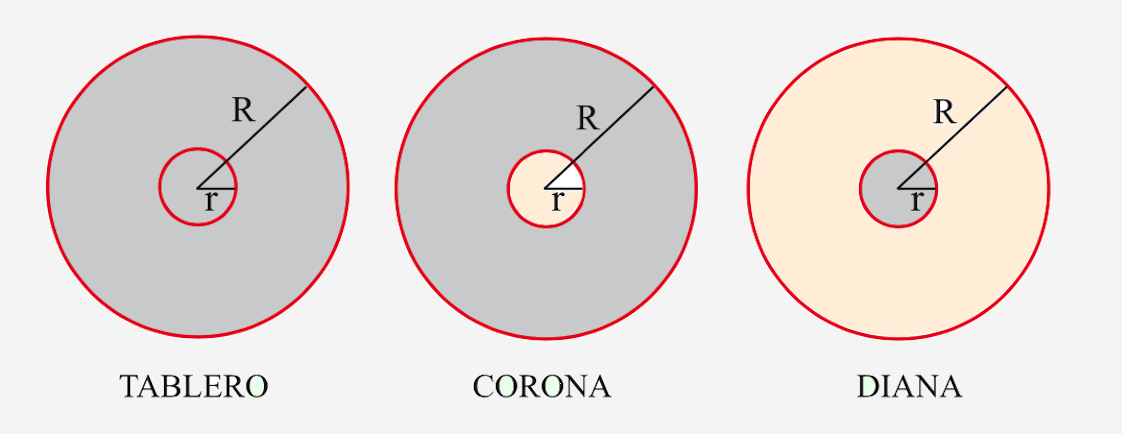
\includegraphics[width=.75\textwidth]{imagenes/imagenes02/T02IM51.png}
	\end{figure}

Donde la palabra `tablero' representa el suceso ``dar en el tablero''; la palabra `diana', ``dar en la diana''; etc. 		
\end{ejer}
\end{ejemplo}

Una vez impactado el tablero, la probabilidad de hacer diana o corona será proporcional a la fracción de las áreas de estas zonas ($A_D,\ A_C$) respecto a la del tablero ($A_T$)

$A_T=\pi R^2;\qquad A_C=\pi (R^2-r^2); \qquad A_D=\pi r^2$

$p(C|T)=\dfrac{\cancel{\pi} (R^2-r^2)}{\cancel{\pi} R^2}=1-\dfrac{r^2}{R^2}; \qquad
p(D|T)=\dfrac{\cancel{\pi} (r^2)}{\cancel{\pi} R^2}=\dfrac{r^2}{R^2}$

Representamos las distintas opciones y sus probabilidades en el siguiente árbol. Llamamos $D$ al suceso 'dar en la diana', $D|T$ a `dar en la diana sabiendo que se ha dado en el tablero', etc.

\begin{tikzpicture}[grow=right, sloped]

% Set the overall layout of the tree
\tikzstyle{level 1}=[level distance=4.5cm, sibling distance=3cm]
\tikzstyle{level 2}=[level distance=6.5cm, sibling distance=3cm]


% Define styles for bags and leafs
\tikzstyle{bag} = [text width=4em, text centered]
\tikzstyle{end} = [circle, minimum width=1pt,fill, inner sep=0pt]

%Define probabilidades en naranja con rectángulo negro de bordes redondeados
\tikzstyle{aristas}=[rectangle, rounded corners=2pt, fill=orange!20, draw=black, font=\small]

\node{}
    child{
    	node{no Tablero $\quad \to 0.1$}
    	edge from parent
    	node[aristas]{$0.1$}
    }
    child{
    	node{Tablero}
    		child{
    		node{Diana: $\ \to 0.9 \cdot \dfrac{r^2}{R^2}$}
    		edge from parent
    		node[aristas]{$\dfrac {r^2}{R^2}$}
    		}
    		child{
    		node{Corona: $\ \to 0.9 \cdot \left( 1- \dfrac{r^2}{R^2} \right) $}
    		edge from parent
    		node[aristas]{$\dfrac {R^2-r^2}{R^2}$}
    		}
    	edge from parent
    	node[aristas]{$0.9$}
    }
	;
\end{tikzpicture}

\begin{multicols}{3}
\begin{small}
$p(C)=0.9\cdot \left( 1-\dfrac {r^2}{R^2} \right)$

$p(D|T)= \dfrac {0.9(r^2/R^2)}{0.9}=r^2/R^2$

$p((T|C)=\dfrac{0.9(1-r^2/R^2)}{0.9(1-r^2/R^2)}=1$

$p(C|no\ T)=(no\ T|D)=0$

$p(D)=0.9 r^2/R^2$

$p(p(T|D)=1$

$p(D| no\ T)=p(no\ T|C)=0$

$p(C|T)=1-r^2/R^2$
\end{small}
\end{multicols}

\vspace{5mm}
\begin{ejemplo}
\begin{ejer}
Imagina cinco sillas alineadas 1, 2, 3, 4, 5 y que un individuo está sentado inicialmente en la silla central (número 3). Se lanza una moneda al aire y, si el resultado es cara, se desplaza a la silla situada a su derecha, mientras que si el resultado es cruz, se desplaza a la situada a su izquierda. Se realizan sucesivos lanzamientos (y los cambios de silla consecutivos correspondientes) teniendo en cuenta que si tras alguno de ellos llega a sentarse en alguna de las sillas de los extremos (1 o 5), permanecerá sentado en ella con independencia de los resultados de los lanzamientos posteriores. Se pide:

a) Dibujar el diagrama de árbol para cuatro lanzamientos de moneda.

b) La probabilidad de que tras los tres primeros lanzamientos esté sentado de nuevo en la silla central (3).

c) La probabilidad de que tras los tres primeros lanzamientos esté sentado en alguna de las sillas de los extremos (1 o 5).

d) La probabilidad de que tras los cuatro primeros lanzamientos esté sentado en alguna de las sillas de los extremos (1 o 5).
\end{ejer}
\end{ejemplo}

La siguiente figura ilustra la resolución del problema. Hemos colocado un \textcolor{green}{$\boldsymbol{+}$} en los casos en que el individuo queda sentado en las silla 1 o 5 tras 3 lanzamientos y un \textcolor{red}{$\boldsymbol{+}$}cuando queda sentado en las sillas 1 o 5 tras el cuarto.

	\begin{figure}[H]
		\centering
		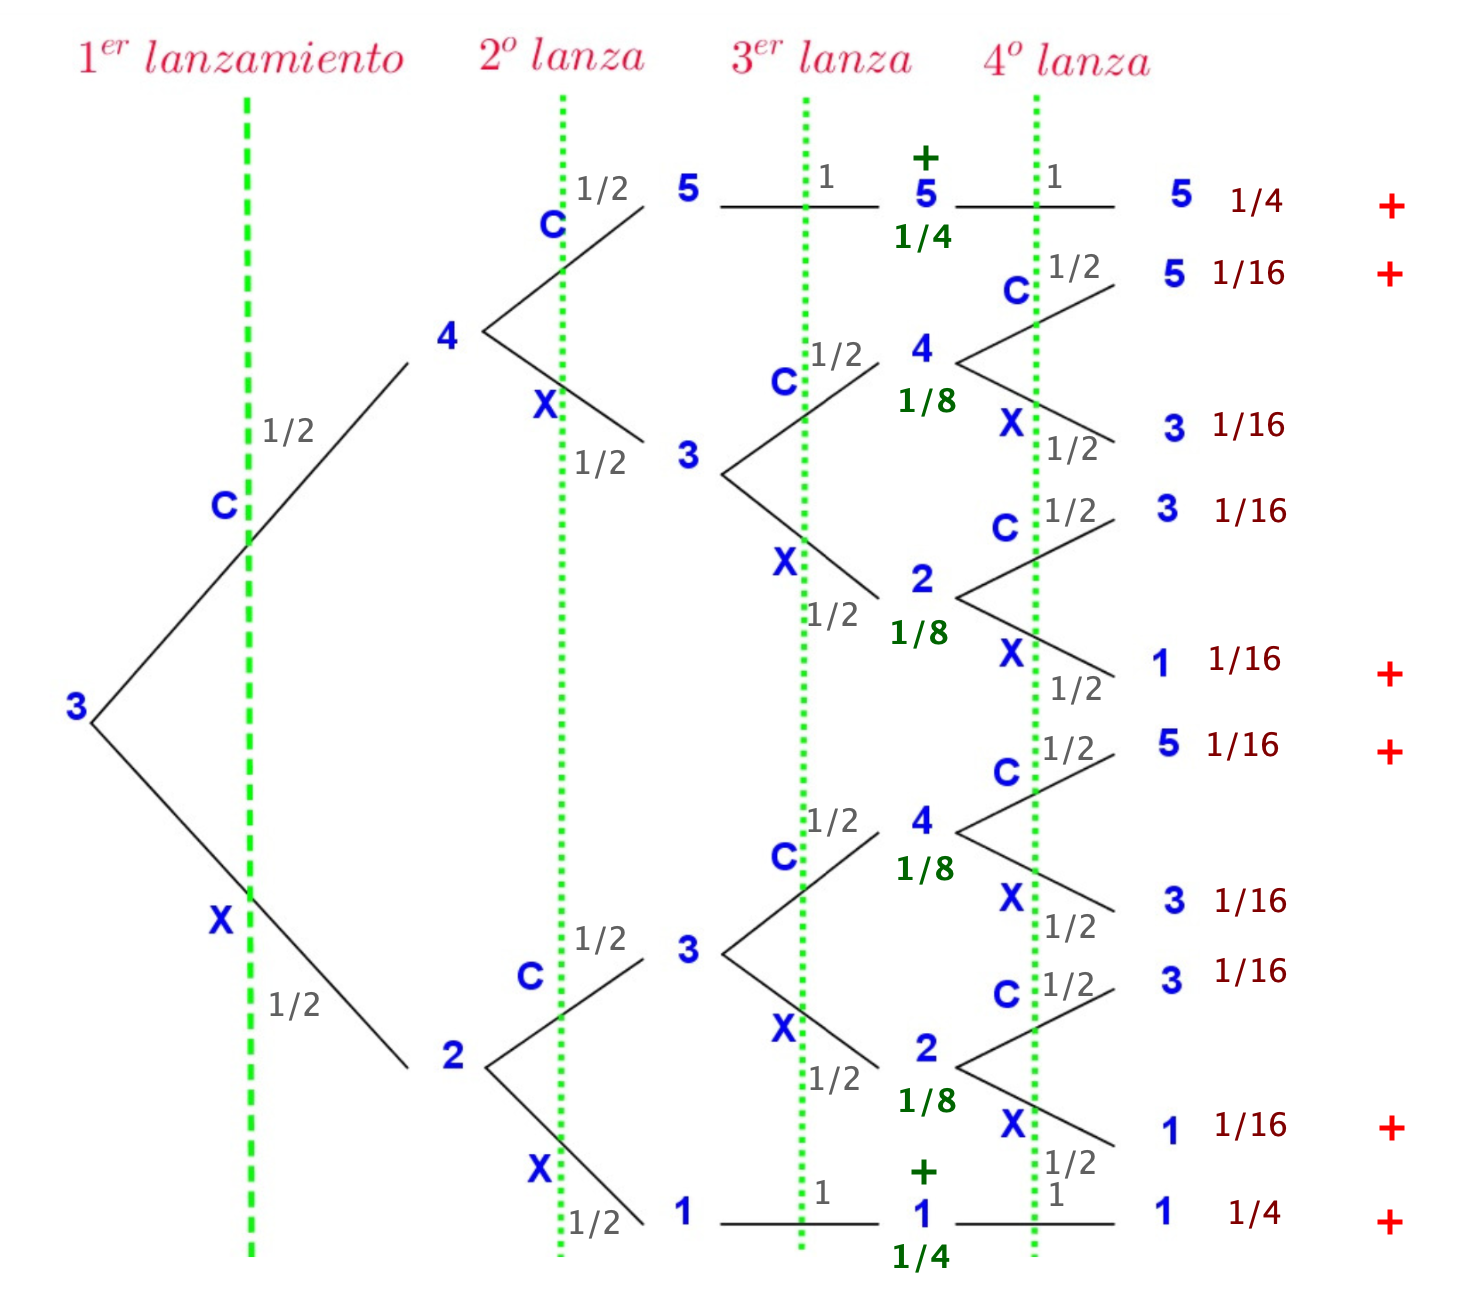
\includegraphics[width=1\textwidth]{imagenes/imagenes02/T02IM52.png}
	\end{figure}
	
$p(\text{silla 3 tras 3 lanzamientos})=0$, tras tres lanzamientos se encuentra en las sillas 1, 2, 4 o 5, nunca en la 3.

$p(\text{silla 1 o 5 tras 3 lanzamientos})=\frac 1 4 + \frac 1 4 = \dfrac 1 2$

$p(\text{silla 1 o 5 tras 4 lanzamientos})=\frac 1 4+4\cdot \frac 1 {16} + \frac 1 4=\dfrac 3 4$


\vspace{1cm}
\begin{adjustwidth}{50pt}{50pt}
	\textcolor{gris}{\rule{70mm}{0.1mm}}
	
	\begin{destacado}
	\textbf{\emph{Los siguientes problemas (`machaca', sin enunciado literario) se pueden resolver aplicando lass fórmulas vistas en el tema, pero es mucho más fácil resolverlos si nos ayudamos del correspondiente diagrama de Venn.}}
	\end{destacado}
	\begin{flushright}
	\rule{70mm}{0.1mm}	
	\end{flushright}
\end{adjustwidth}
\vspace{1cm}



\vspace{5mm}
\begin{ejemplo}
\begin{ejer}
Sean $A$ y $B$ dos sucesos de un espacio de probabilidad tales que: $P[A'] = 0.6 ; \ P[B] = 0.3 ; \ P[A' \cup B'] = 0.9$

a) ?`Son independientes $A$ y $B$?, ?`son incompatibles?

b) Calcula $P[A | B']$.	
\end{ejer}
\end{ejemplo}
Aunque es sencillo volver a recorcar con un diagrama de Venn que $(A' \cup B')$ es el complementario de $(A\cap B)$ (es una de las leyes de Morgan), presentamos la siguiente figura que será de utilidad en los problemas 'machaca'.


	\begin{figure}[H]
		\centering
		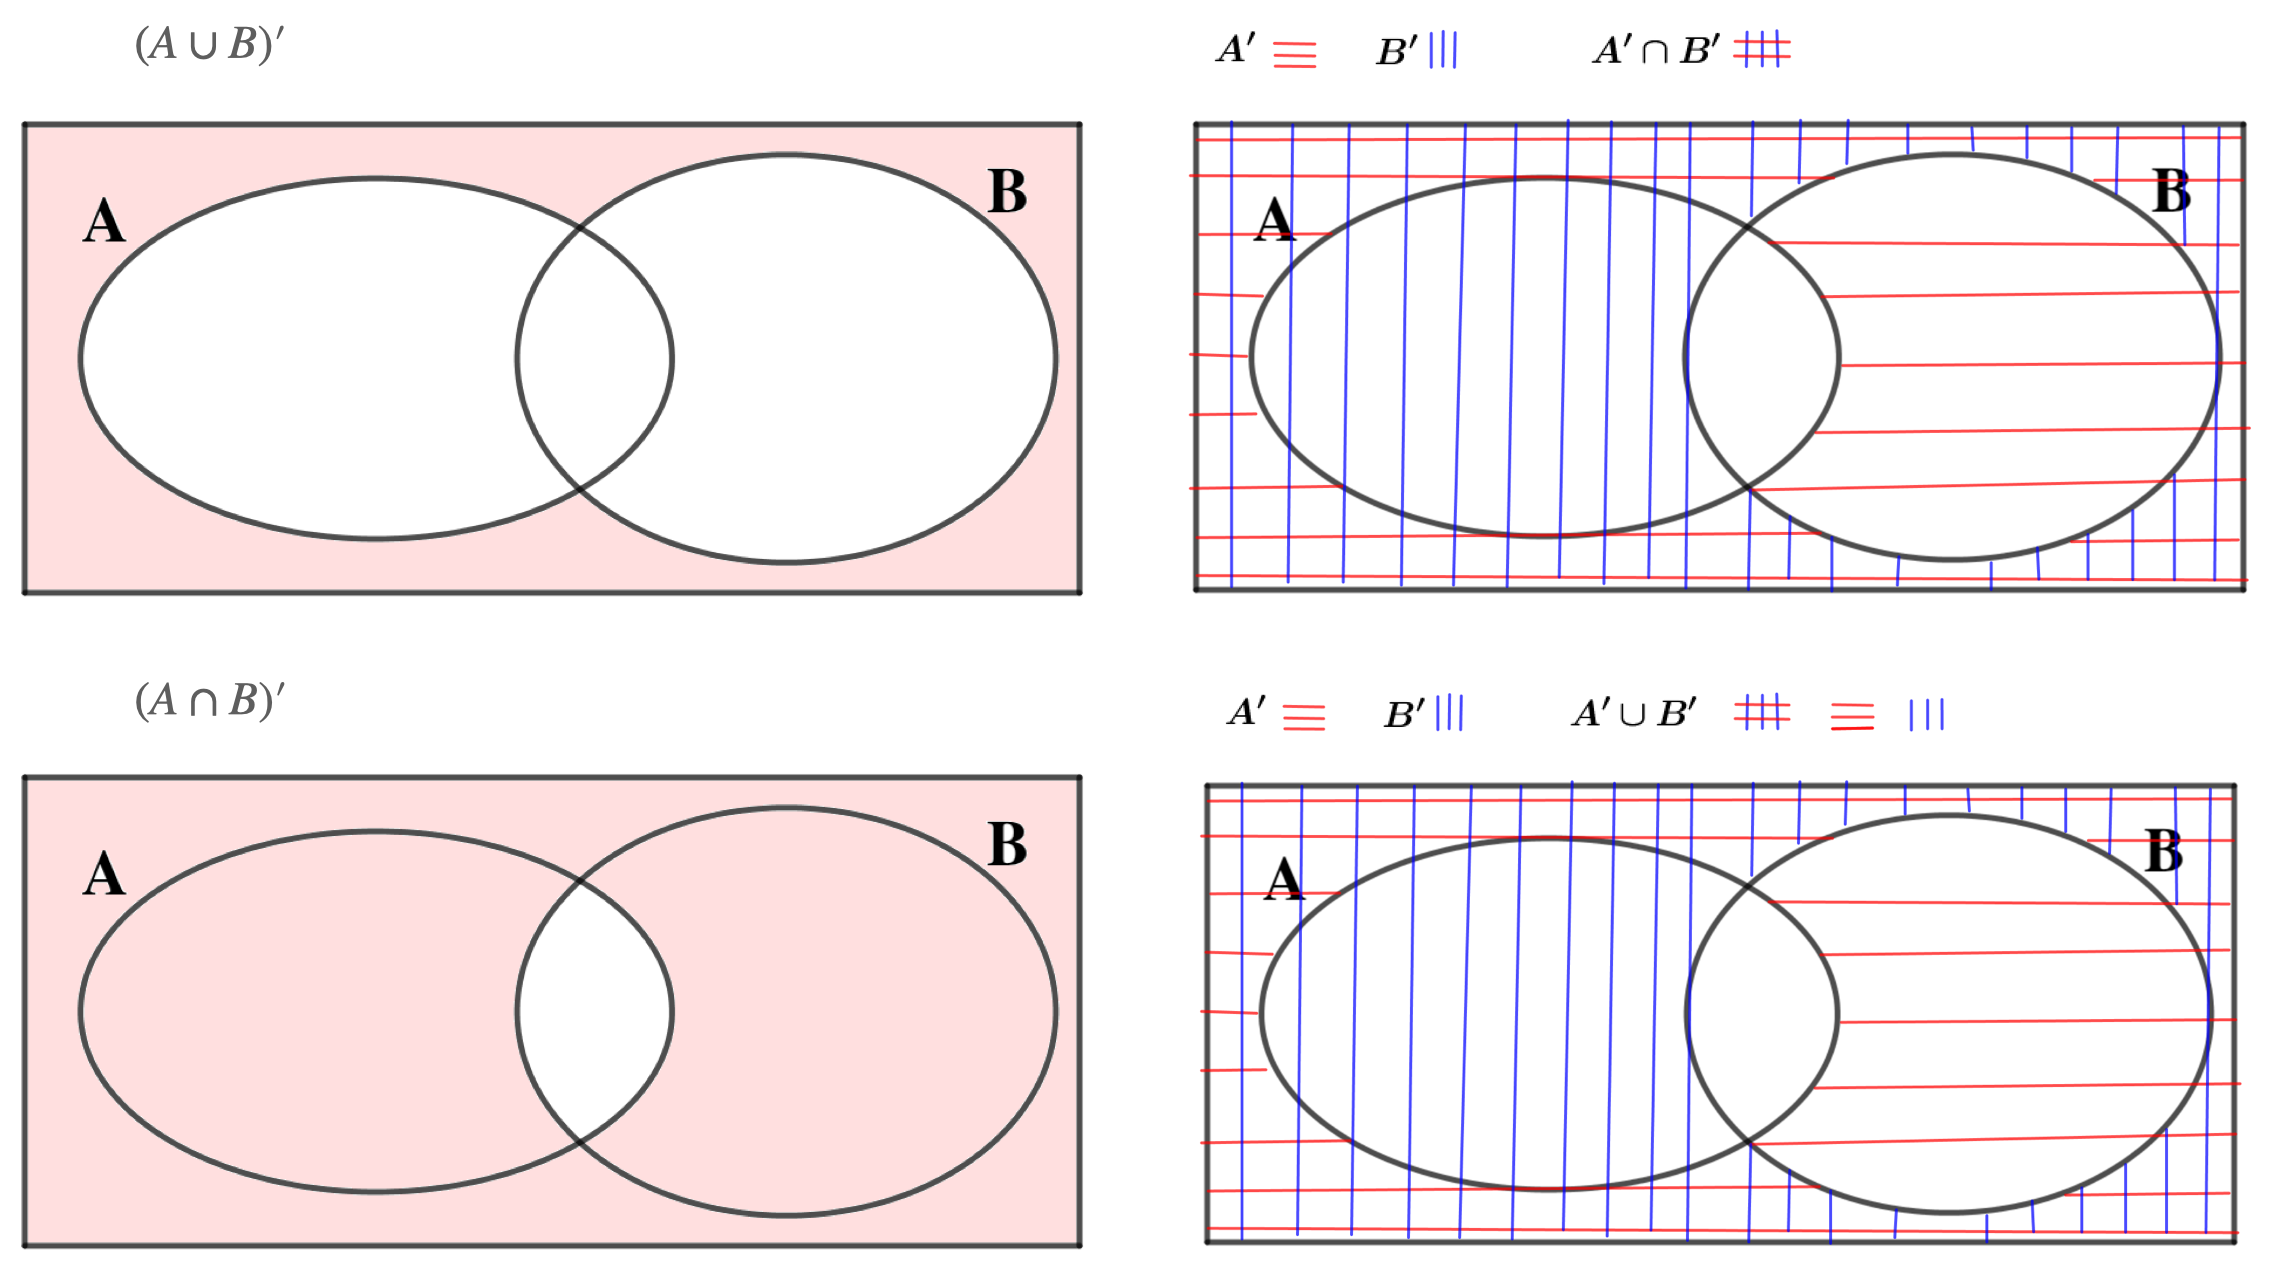
\includegraphics[width=.75\textwidth]{imagenes/imagenes02/T02IM38.png}
		\caption*{Leyes de Morgan}
	\end{figure}


$p(A')=0.6\to p(A)=0.4;\qquad p(A\cap B)=1-p(A'\cup B')=1-0.9=0.1$

Si $P(A)=0.4$ y $P(A\cap B)=0.1 \to  p(A-B)= 0.4-0.1=0.3$

Análogamente, $\ p(B-A)=0.3.0.1=0.2$

La región externa, $\ p(A\cup B)'=1-0.3-0.1-0.2=0.4$

	\begin{figure}[H]
		\centering
		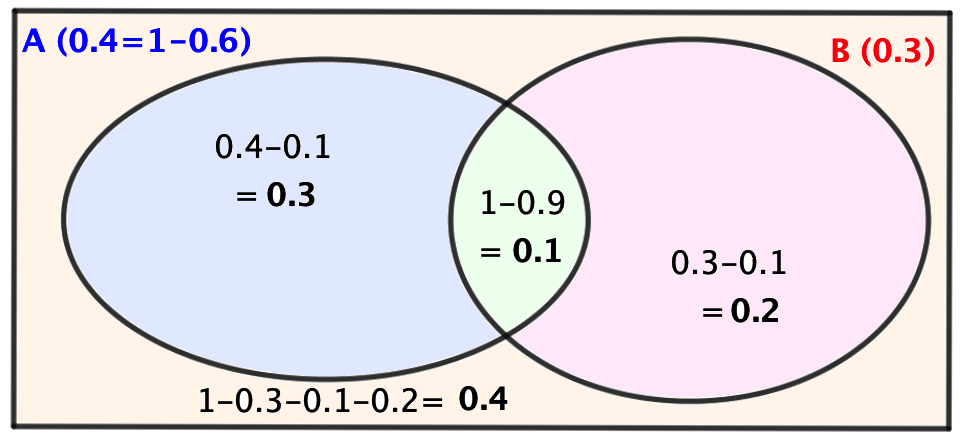
\includegraphics[width=.6\textwidth]{imagenes/imagenes02/T02IM39.png}
	\end{figure}
$p(A)=0.4;\qquad     p(A|B)=0.1/0.3=0.33 \to p(A)\neq p(A|B) \to A \text{ y } B$ son dependientes.

$p(A\cap B)=0.1\neq 0 \to A \text{ y } B$ son compatibles.

De la última figura, B' `ha ocurrido' en 0.3+0.4=0.7 `ocasiones', de ellas, A `ha ocurrido' en solo 0.3 `ocasiones', por lo que: $p(A|B')=0.3/0.7=0.43$. Para facilitar el cálculo basta con que en el diagrama, al saber que ha ocurrido B' (el suceso que condiciona), tapes con tu mano todo el suceso B. Te queda solo 0.3 y 0.4. De ellos, en 0.3 ocurre A.

Con un razonamiento análogo, se puede calcular $p(A'|B)$ (si ocurre B, nos quedamos solo con B e ignoramos el resto, tenemos 0.1 -ocurre A- y 0.2 -ocurre A'-):

$p(A'|B)=0.2/(0.1+0.2)=0.2/0.3=0.67
\quad \text{ y } \quad  
p(A'|B')=0.4/(0.3+0.4)=0.4/0.7=0.57$

\vspace{5mm}
\begin{ejemplo}
\begin{ejer}
Sabiendo que $p(A)=0.5;\ \ p(B')=0.6;\ \ p(A'\cap B')=0.25$, calcula:
$p(A|B); \ \  p(A'|B); \ \ p(A|B'); \ \  p(A'|B')$. Calcula, también, $p(A\cap B|A\cup B)$.
\end{ejer}
\end{ejemplo}
$p(B')=0.6 \to p(B)=0.4$

O bien dibujándonos quién es $A'\cap B'$ o bien recordando la figura ``Leyes de Morgan'' del ejercicio 2.20, tenemos que $A'\cap B'$ representa la región externa a A y a B. Ponemos los datos en nuestro diagrama de Venn y nos vemos obligado a llamar $x=p(A\cap B)$, pues nos es desconocida. Con esto, $p(A-B)=0.5-x$ y $p(B-A)=0.4-x$. Puesto que la probabilidad total ha de ser $1:\ 0.5-x+x+0.4-x+0.25=1 \to x=0.15$ y ya podemos completar nuestro diagrama de Venn. !`Ahora, que nos pregunten lo que quieran!

	\begin{figure}[H]
		\centering
		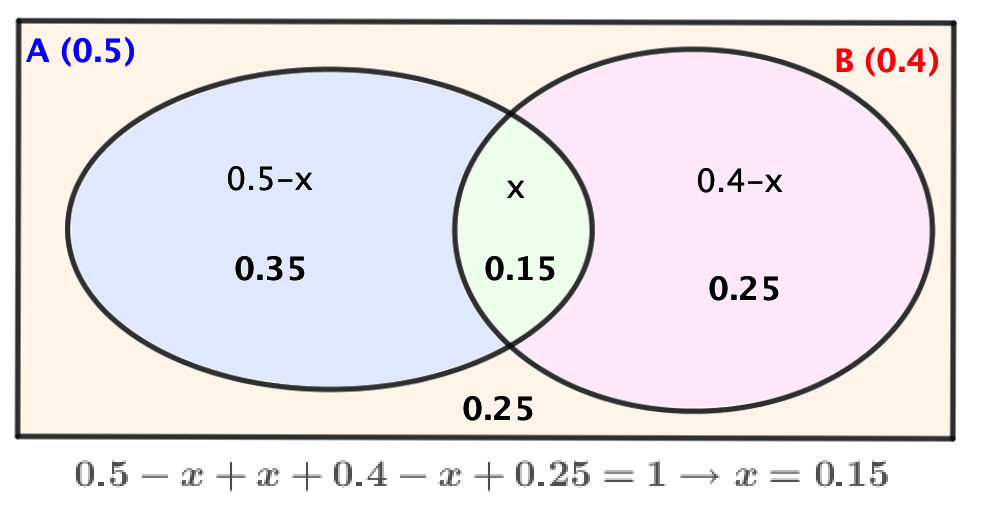
\includegraphics[width=.6\textwidth]{imagenes/imagenes02/T02IM40.png}
	\end{figure}

Para calcular las probabilidades condicionadas a B, nos centramos solo en B y observamos que hay 0.15 y 0.25 posibilidades, en las primeras ocurre A y en las segundas no (ocurre B'). Para probabilidades condicionadas a B' nos centramos en lo que no es B (podemos tapar el conjunto B con nuestra mano) y observamos que quedan 0.35 y 0.25 posibilidades, en las primeras ocurre A y en las segundas A'.


$p(A|B)=0.15/(0.15+0.25)=0.375; \qquad \ p(A'|B)=0.25(0.15+0.25)=0.625$

$p(A|B')=0.35/(0.35+0.25)=0.583;\qquad p(A'|B')=0.25/(0.35+0.25)=0.417$


Para calcular $p(A\cap B|A\cup B)$, puesto que sabemos que se ha verificado el suceso $A\cup B$, tenemos 0.35 (ocurre solo A) más 0.15 (ocurren A y B simultáneamente) más 0.25 (ocurre solo B), luego:
$\ p(A\cap B|A\cup B)=0.15/(0.35+0.15+0.25=0.12/0.75=0.200$

\vspace{5mm}
\begin{ejemplo}
\begin{ejer}
Dos sucesos tienen la misma probabilidad de ocurrir, 0.5. La probabilidad de que ocurra uno de los sucesos sabiendo que ha ocurrido el otro es 0.3. ?`Cuál es la probabilidad de que no ocurra ninguno de los sucesos?
\end{ejer}
\end{ejemplo}

Tenemos que $p(A)=p(B)=0.5$ y que, por ejemplo, $p(A|B)=0.3=\dfrac{p(A\cap B)}{p(B)}= \dfrac {p(A\cap B)} {0.5}  \to p(A\cap B)=0.5\cdot 0.3=0.15$

 \textcolor{gris}{Lo que es compatible con que $0.3=p(B|A)=\dfrac{p(A\cap B)}{p(A)}=\dfrac{0.15}{0.5}=0.3$. }  

Ahora, $p(A\cup B)=p(A)+p(B)-p(A\cap B)=0.5+0.5-0.15=0.85$

De donde, $p(A'\cap B')=p(A\cup B)'=1-p(A\cup B)=1-0.85=01.5$

\vspace{-4mm} \begin{center} \textcolor{gris}{\rule{70mm}{0.1mm}} \end{center}
 
 Con la ayuda de un diagrama de Venn.
	\begin{figure}[H]
		\centering
		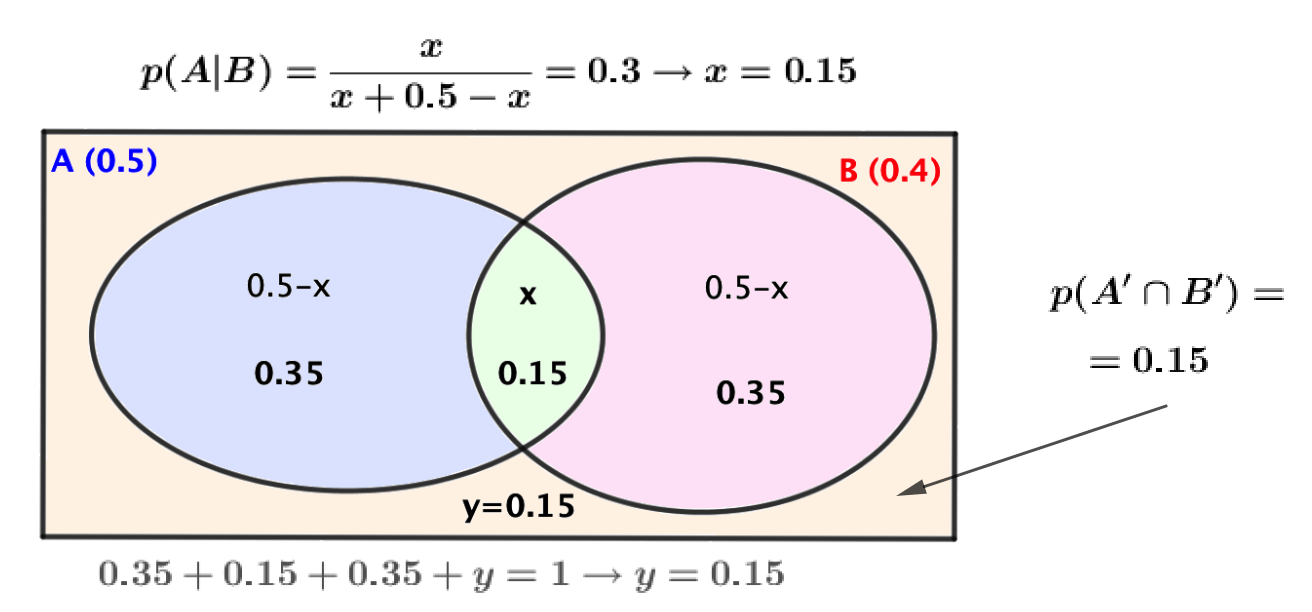
\includegraphics[width=.75\textwidth]{imagenes/imagenes02/T02IM41.png}
	\end{figure}

\vspace{5mm}
\begin{ejemplo}
\begin{ejer}
Dados dos sucesos $A$ y $B$, sabemos que $p(A\cap B)=0.1;\ \ p(A\cup B)=0.7$ y que $p(A|B)=0.2$. Calcula $p(A)$ y $p(B)$ y di si los sucesos $A$ y $B$ son independientes y/o incompatibles.	
\end{ejer}
\end{ejemplo}
	
	\begin{figure}[H]
		\centering
		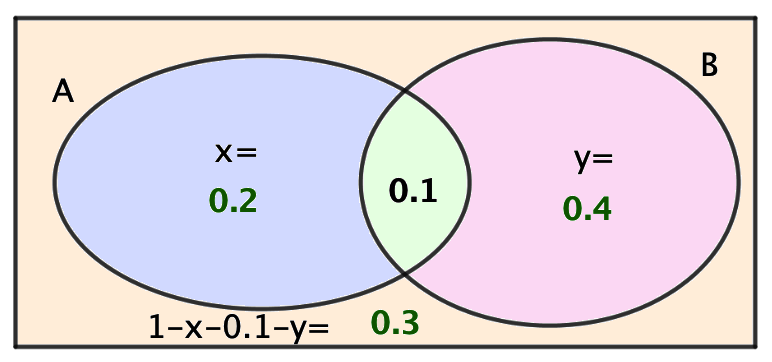
\includegraphics[width=.6\textwidth]{imagenes/imagenes02/T02IM42.png}
	\end{figure}

Hemos llamado $\ x=p(A-B)\ $ e $\ y=p(B-A)$.

$p(A|B)=0.2 \to \dfrac{0.1}{0.1+y}=0.2 \to y=0.4$

$p(A\cup B)=0.7 \to 0.7= x+0.1+0.4 \to x=0.2$

Con esto, $\ p(A)=0.2+0.1=0.3;\qquad p(B)=0.1+0.4=0.5$

Como $\ p(A\cap B)=0.1\neq 0 \to A\text{ y } B\ $ son compatibles.

Como $\ p(A)=0.3 \neq 0.2 =p(A|B) \to A\text{ y } B\ $ son dependientes.

\vspace{5mm}
\begin{ejemplo}
\begin{ejer}
Sabemos que $p(B|A)=0.9;\ \ p(A|B)=0.2 \ \text{ y } \ p(A)=0.1$. Calcula  $p(B)$ y di si los sucesos $A$ y $B$ son independientes y/o incompatibles. ?`Qué vale $p(A\cup B')$?
\end{ejer}
\end{ejemplo}

	\begin{figure}[H]
		\centering
		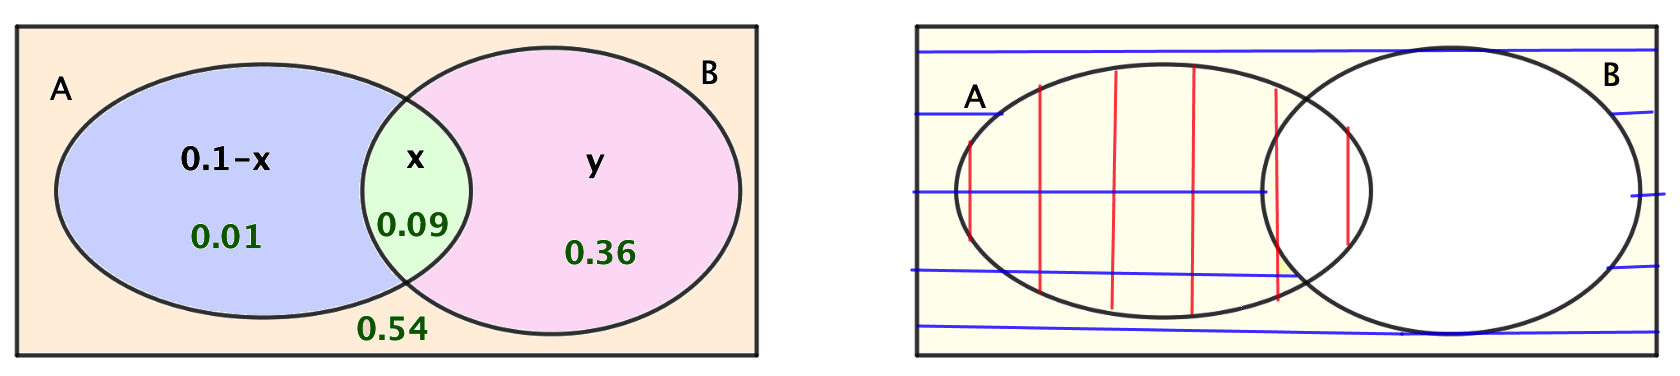
\includegraphics[width=1\textwidth]{imagenes/imagenes02/T02IM43.png}
	\end{figure}

Llamamos $x=p(A\cap B)$, como $p(A)=0.1\to p(B-A)=0.1-x$. Llamamos $y=p(B-A)$.

$P(B|A)=0.9 \to \dfrac{x}{0.1-x+x}=0.9 \to x=0.09$

$P(A|B)=0.2 \to \dfrac{0.09}{0.09+y}=0.2 \to y=0.36$

La zona externa, $p(AUB)'=1-0.01-0.09-0.36=0.64$. !`Listo!

$p(B)=0.09+0.36=0.45$

$p(A\cap B)=0.09\neq 0 \to $ compatibles.

$p(B|A)=0.9\neq 0.45=p(B) \to $ dependientes.

En el dibujo de la derecha hemos representado $A$ en vertical y $B'$ en horizontal. Como buscamos la unión, estamos interesados en todo lo rayado, vertical u horizontalmente, la zona amarilla (si buscásemos la intersección nos interesaría la zona en que se cruzan las líneas, $A-B$).

De est modo, $\ p(A\cup B')=1-0.36=0.64$


\vspace{1cm}
\begin{adjustwidth}{50pt}{50pt}
	\textcolor{gris}{\rule{70mm}{0.1mm}}
	
	\begin{destacado}
	\textbf{\emph{Los siguientes problemas nos preparan para el siguiente tema de distribuciones de probabilidad. En concreto, para la distribución binomial de probabilidad.}}
	\end{destacado}
	\begin{flushright}
	\rule{70mm}{0.1mm}	
	\end{flushright}
\end{adjustwidth}
\vspace{1cm}



\begin{ejemplo}
\begin{ejer}
Un arquero dispone de 3 flechas en su carcaj. Su probabalidad de hacer diana es constante y vale 0.8; una vez conseguida una diana, acaba el juego.	

?`Cuál es la probabilidad que que el arquero haga diana al segundo intento? ?`Y de que haga diana en algún intento? 

?`Cuál es la probabilidad de fallar todos sus intentos si dispone de 5 flechas en su carcaj?
\end{ejer}
\end{ejemplo}

\begin{center}
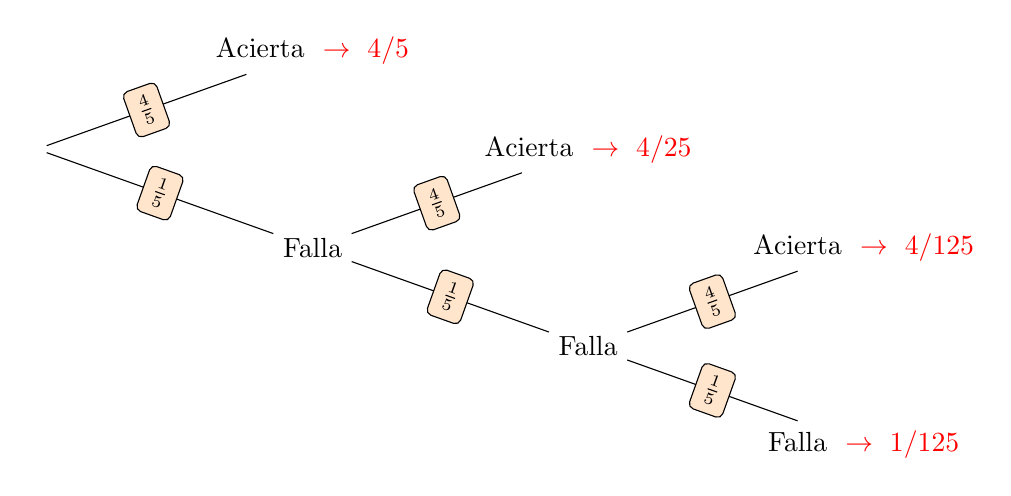
\begin{tikzpicture}[grow=right, sloped]

% Set the overall layout of the tree
\tikzstyle{level 1}=[level distance=3.5cm, sibling distance=2.5cm]
\tikzstyle{level 2}=[level distance=3.5cm, sibling distance=2.5cm]
\tikzstyle{level 3}=[level distance=3.5cm, sibling distance=2.5cm]

% Define styles for bags and leafs
\tikzstyle{bag} = [text width=4em, text centered]
\tikzstyle{end} = [circle, minimum width=1pt,fill, inner sep=0pt]

%Define probabilidades en naranja con rectángulo negro de bordes redondeados
\tikzstyle{aristas}=[rectangle, rounded corners=2pt, fill=orange!20, draw=black, font=\small]

\node{}
    child{
   		node{Falla}
   			child{
   				node{Falla}
   					child{
   						node{Falla $\ \textcolor{red}{\to \ 1/125}$}
   						edge from parent
    					node[aristas]{$\frac  1 5$}
    				}
    				child{
    					node{Acierta $\ \textcolor{red}{\to \ 4/125}$}
    					edge from parent
    					node[aristas]{$\frac 4 5$}
    				}
    			edge from parent
    			node[aristas]{$\frac 1 5$}
   			 }
   		 	child{
    			node{Acierta $\ \textcolor{red}{\to \ 4/25}$}
    			edge from parent
    			node[aristas]{$\frac 4 5$}
   			 }
   		edge from parent
    	node[aristas]{$\frac 1 5$}
    }
    child{
    	node{Acierta $\ \textcolor{red}{\to \ 4/5}$}
    	edge from parent
    	node[aristas]{$\frac 4 5$}
    }
    ;  
\end{tikzpicture}
\end{center}

$p(\text{acierto 2 intento})=4/25$

$p(\text{algún acierto})=1-p(\text{ningún acierto})=1-1/125=124/125$

Con cinco flechas: $p(\text{algún acierto})=1-1/5^5=3124/3125$

\vspace{5mm}
\begin{ejemplo}
\begin{ejer}
Un jugador de tenis tiene una probabilidad de 0.4, constante, de ganar una partida, si juega cuatro partidas, calcula la probabilidad de que gane más de la mitad.	
\end{ejer}
\end{ejemplo}

Para resolver el problema con un árbol necesitaríamos $2 \cdot 2 \cdot 2 \cdot 2=2¿4=16$ ramas, excesivo. Intentemos resolver el problema razonando.

En cada jugada, independientemente de jugadas anteriores, la probabilidad de ganar es $p(G)=0.4$ y la de perder $p(P)=0.6$. El jugador ganará más de la mitad de las partidas si gana 3 o 4 partidas.

--- Ganar 3 partidas es tanto como perder una sola, ésta puede ser la primera, la segunda, la tercera o la cuarta.

Calculemos la probabilidad de perder la primera y ganar las restantes: $PGGG\to 0.6\cdot 0.4 \cdot 0.4 \cdot 0.4=0.6\cdot 0.4^3$. Pero la probabilidad de perder en la tercera de las partidas también es: $GGPG\to 0.4\cdot 0.4 \cdot 0.6 \cdot 0.4=0.6\cdot 0.4^3$. Así, para los cuatro casos:

$p(\text{ganar 3 partidas})=p(3)=4\cdot 0.6\cdot 0.4^3$

--- Ganar la cuatro partidas tiene una probabilidad de $GGGG\to 0.4\cdot 0.4 \cdot 0.4 \cdot 0.4=0.4^4$

------ Finalmente, ganar más de la mitas de las partidas $=p(3)+p(4)=4\cdot 0.6\cdot 0.4^3 +0.4^4=0.1792\approx 18\%$.



\vspace{5mm}
\begin{ejemplo}
\begin{ejer}
Un alumno realiza un examen tipo test que consta de 5 preguntas. Cada una de las preguntas tiene tres posibles respuestas, de las que solo una es correcta. Si el alumno aprueba contestando correctamente tres o más preguntas, obtener de forma razonada la probabilidad de que apruebe si escoge las respuestas de cada una de las preguntas completamente al azar	
\end{ejer}
\end{ejemplo}

En esta ocasión, el árbol es aún mayor, de $2^5=32$ ramas. Razonemos de modo análoga al problema anterior.

$p(acertar)=p(A)=1/3; \ \ p(fallar)=p(F)=2/3$.

Aprueba si acierta tres o más: $\ p(aprobar)=p(3)+p(4)+p(5)$, donde con $p(i)$ indicamos la probabilidad de acertar $i$ preguntas.

\textcolor{gris}{El suceso contrario, $p(suspender)=p(0)+p(1)+p(2)$, parece que tiene tantos cálculos como el suceso pedido, por lo que abordamos el problema directamente.}

--- Probabilidad de acertar 3 de las 5 preguntas:

$AAAFF \ \to \ 1/3\cdot 1/3 \cdot 1/3 \cdot 2/3 \cdot 2/3=(1/3)^3\cdot (2/3)^2$

$AAFFA \ \to \ 1/3\cdot 1/3 \cdot 2/3 \cdot 2/3 \cdot 1/3=(1/3)^3\cdot (2/3)^2$

Todas las formas de obtener 3 aciertos y dos fallos tiene la misma probabilidad, $(1/3)^3\cdot (2/3)^2$.

?`Cuántas formas hay de acertar 3 de 5 preguntas? $\ \to \ C_{5}^3=\mqty(5\\2)=\dfrac{5!}{3!\cdot 2!}=10$ \textcolor{gris}{(* Ver cáculo sin usar combinatoria al final del problema)}.

Luego, $\ p(3)=10\cdot (1/3)^3\cdot (2/3)^2$

--- Probabilidad de acertar 4 de la cinco preguntas $\to AAAAF,\ $ $AAAFA,\ $ $AAFAA,\ $ $AFAAA,\ $ $FAAAA$, 5 formas distintas ($C_5^1=C_5^4=5$), todas ellas con la misma probabilidad, 4 aciertos y 1 fallo, $(1/3)^4\cdot (2/3)$.

--- Probabilidad de acertarlas todas, una sola forma ($C_5^5=C_5^0=1$, 5 aciertos, 0 fallos), con probabilidad $(1/3)^5)$

------ Finalmente,

$p(aprobar)=p(3)+p(4)+p(5)=10 \cdot (1/3)^3 \cdot (2/3)^2+ \cdot 5 \cdot (1/3)^4 \cdot (2/3) + 1 \cdot (1/3)^5=0.2099\approx 21\%$

\vspace{1cm} 

\textcolor{gris}{\rule{100mm}{0.1mm}}

\textcolor{gris}{Las distintas formas de ordenar 3 A y 2 F son:}

\textcolor{gris}{Si las F están juntas: FFAAA; AFFAA; AAFFA; AAAFF}

\textcolor{gris}{Si las F dejan un espacio entre ellas: FAFAA; AFAFA; AAFAF}

\textcolor{gris}{Si las F dejan dos espacios entre sí: FAAFA; AFAAF}

\textcolor{gris}{Si dejan 3 espcios entre ellas: FAAAF}

\textcolor{gris}{En total, 10 formas distintas}

\textcolor{gris}{Es recomendable consultar el apéndice \ref{combinatoria} de combinatoria.}
 
\begin{flushright} \rule{100mm}{0.1mm} \end{flushright}

\vspace{1cm}

\begin{adjustwidth}{50pt}{50pt}
	\textcolor{gris}{\rule{70mm}{0.1mm}}
	
	\begin{destacado}
	\textbf{\emph{Para acabar los problemas resueltos de probabilidad, presentamos los `tres problemas clásicos del caballero de Méré'' que dieron lugar a la teoría de la probabilidad.}}\footnote{Antoine Gombard, Caballero De Meré y experto jugador, planteó a  Blaise Pascal tres problemas sobre apuestas. En 1654, Pascal y Pierre de Fermat (1601-1665) mantuvieron abundante correspondencia sobre estos problemas. Las soluciones que entre los dos encontraron sentaron las bases del Cálculo de Probabilidades.}
	\end{destacado}
	\begin{flushright}
	\rule{70mm}{0.1mm}	
	\end{flushright}
\end{adjustwidth}
\vspace{1cm}

\vspace{5mm}
\begin{ejemplo}
\begin{ejer}
?`Es ventajoso apostar por el resultado de obtener, al menos un 6, en una serie de 4 lanzamientos de un dado?
\end{ejer}
\end{ejemplo}
Suceso contrario, $p(\text{ningún 6 en 4 lanzamientos})=(5/6)^4$,

luego  $p(\text{algún 6 en 4 lanzamientos})=1-(5/6)^4=0.5168>50\%$, sí es ventajoso.

\vspace{5mm}
\begin{ejemplo}
\begin{ejer}
?`Es ventajoso apostar por el resultado de obtener al menos un doble 6 en una serie de 24 lanzamientos con un par de dados?	
\end{ejer}
\end{ejemplo}
$p(\text{doble 6 al lanzar un par de dados})=p(6,6)=1/36 \to p(no-6,6)=35/36$

$p(\text{obtener ningún doble 6 en 24 lanzamientos})=(35/36)^{24}=0.5086$

Luego, $p(\text{obtener algún doble 6 en 24 lanzamientos})=1-(35/36)^{24}=0.4914<50\%$, no es ventajoso.


\vspace{5mm}
\begin{ejemplo}
\begin{ejer}
\textbf{La apuesta interrumpida:} A y B apuestan, 32 escudos de oro cada uno, a cara o cruz lanzando una moneda. El primero que llegue a obtener 5 puntos gana la apuesta y se lleva todo el dinero (A gana si sale cara y B si sale cruz, el primero en llegar a 5 victorias gana). El juego se interrumpe por causas de fuerza mayor cuando A tiene 4 puntos y B 3 puntos. ?`Cómo deben repartirse el dinero?
\end{ejer}
\end{ejemplo}

Al principio los jugadores A y B están (4,3) (A gana 4 partidas y B gana 3). Ambos jugadores tienen la misma probabilidad de ganar (1/2). Si sale cara, gana A y se ponen (5,3); concluye la partida. Si gana B están (4,4) y hacen un segundo lanzamiento. Representamos la situación con el siguiente diagrama de árbol.

\begin{center}
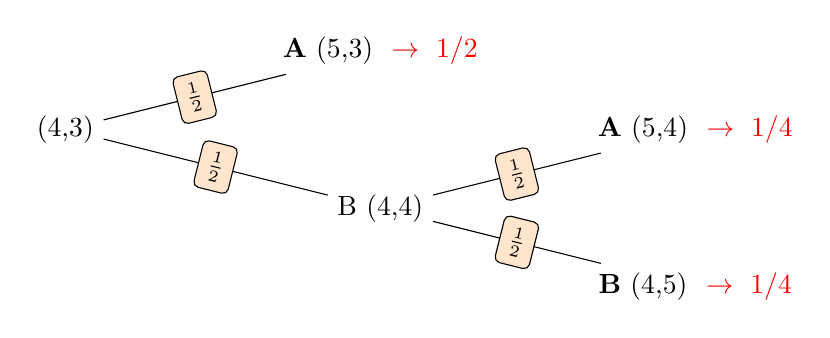
\begin{tikzpicture}[grow=right, sloped]

% Set the overall layout of the tree
\tikzstyle{level 1}=[level distance=4cm, sibling distance=2cm]
\tikzstyle{level 2}=[level distance=4cm, sibling distance=2cm]


% Define styles for bags and leafs
\tikzstyle{bag} = [text width=4em, text centered]
\tikzstyle{end} = [circle, minimum width=1pt,fill, inner sep=0pt]

%Define probabilidades en naranja con rectángulo negro de bordes redondeados
\tikzstyle{aristas}=[rectangle, rounded corners=2pt, fill=orange!20, draw=black, font=\small]

\node{(4,3)}
    child{
   		node{B (4,4)}
   			child{
   				node{\textbf{B} (4,5) $\ \textcolor{red}{\to \ 1/4}$}
    			edge from parent
    			node[aristas]{$\frac 1 2$}
   			 }
   		 	child{
    			node{\textbf{A} (5,4) $\ \textcolor{red}{\to \ 1/4}$}
    			edge from parent
    			node[aristas]{$\frac 1 2$}
   			 }
   		edge from parent
    	node[aristas]{$\frac 1 2$}
    }
    child{
    	node{\textbf{A} (5,3) $\ \textcolor{red}{\to \ 1/2}$}
    	edge from parent
    	node[aristas]{$\frac 1 2$}
    }
    ;  
\end{tikzpicture}
\end{center}

Probabilidad de ganar A: $\ p(A)=1/2+1/4=3/4=75\ $, probabilidad de ganar B: $\ p(B)=25\%$. Los jugadores repartirán la apuesta proporcionalmente a las posibilidades que tienen de ganar:

Para A: $\ 75\% \text{ de } 64 \text{\ doblones\ }= 48 \text{\ doblones\ };\quad $ Para B: $\ 25\% \text{ de } 64 \text{\ doblones\ } = 16 \text{\ doblones }$.






\begin{comment}
\vspace{5mm}
\begin{ejemplo}
\begin{ejer}
enunciado	
\end{ejer}
\end{ejemplo}
resolución	
\end{comment}






\subsection{Problemas propuestos (con solución)}

\begin{adjustwidth}{5mm}{5mm}

\begin{enumerate}[PB. 1. ]


\item Un aparato está formado por dos partes A y B. El proceso de fabricación es tal que la probabilidad de un defecto en A es 0,06 y la probabilidad de un defecto en B es 0,07. ¿Cuál es la probabilidad de que el producto no sea defectuoso? 

\hspace{-1cm}\rotatebox{180}{\leftline{\textcolor{gris}{0.8742}}}\vspace{1cm}



\item La baraja española consta de diez cartas de oros, diez cartas de copas, diez cartas de espadas y diez cartas de bastos. Se extraen tres cartas. Averiguar razonadamente cuál es la probabilidad de que al menos una de las cartas de oros en los siguientes supuestos: 

a) No se devuelven las cartas después d la extracción.

b) Después d cada extracción se devuelve la carta a la baraja antes de la extracción siguiente. 

\hspace{-1cm}\rotatebox{180}{\leftline{\textcolor{gris}{Piensa en el suceso contrario. $a)\ 0.4375;\ \ b) 0.4423$}}}\vspace{1cm}




\item La ciudad A tiene el triple de habitantes que la ciudad B. Un 10\% de habitantes de la ciudad A son alérgicos y un 30\% de habitantes de la ciudad B son alérgicos. Se selecciona un ciudadano sin saber de que ciudad es. Deducir razonadamente cuál es la probabilidad de que sea alérgico.

Entre todos los habitantes alérgicos de ambas ciudades se selecciona un ciudadano. ¿Cuál es la probabilidad de que sea de la ciudad A?. 

\hspace{-1cm}\rotatebox{180}{\leftline{\textcolor{gris}{0.15; 0.50}}}\vspace{1cm}

\item En un aparato de radio hay presintonizadas tres emisoras A, B y C que emiten durante todo el día. La emisora A siempre ofrece música, mientras que la B y la C lo hacen la mitad de tiempo de emisión. Al encender la radio se sintoniza indistintamente cualquiera de las tres emisoras. 

a) Obtener de forma razonada la probabilidad de que al encender la radio escuchemos música. 

b) Si al poner la radio no escuchamos música, calcular de forma razonada cuál es la probabilidad de que esté sintonizada la emisora B. 

\hspace{-1cm}\rotatebox{180}{\leftline{\textcolor{gris}{sol}}}\vspace{1cm}

\item  ¿Cuál es la probabilidad de obtener 12 al multiplicar los resultaos de dos dados? ¿Y de que la diferencia sea 2?

\hspace{-1cm}\rotatebox{180}{\leftline{\textcolor{gris}{Haz las tablas de doble entrada. $\quad 1/9; \ \ 2/9$}}}\vspace{1cm}


\item  Una fábrica tiene 3 máquinas que fabrican tornillos, la máquina A produce el 50\% del total de los tornillos de la fábrica, la B el 30\% y la C el 20\%. De la máquina A salen un 5\% de tornillos defectuosos, un 4\% de la B y un 2\% de la C. 

a) Calcula la probabilidad de que un tornillo elegido al azar resulte defectuoso.

b) Si sabemos que el tornillo elegido es defectuoso, ¿cuál es la probabilidad de que haya sido fabricado por la máquina C?

\hspace{-1cm}\rotatebox{180}{\leftline{\textcolor{gris}{0.042; 0.095}}}\vspace{1cm}

\item  Sabiendo qu $p(A)=0.3,\ \ p(B)=0.4 \ \text{ y } p(A|B)=0.2$, calcula:

a) $\ p(A’\cup B),\ \ p(B|A),\ \ p(A’\cup B’);\ \ P(A\cap B|A\cup B); $

b) $\ p(A|B),\ \  p(A’|B), \ \  p(A|B’), \ \  p(A’|B’)$

c) ¿Son $A$ y $B$ Independientes?, ¿son incompatibles?
 
\hspace{-1cm}\rotatebox{180}{\leftline{\textcolor{gris}{0.32/0.40; 0.08/0.30; 0.92; 0.08/0.62}}}

\hspace{-1cm}\rotatebox{180}{\leftline{\textcolor{gris}{0.08/0.40; 0.32/0.40; 0.22/0.60; 0.38/0.60}}}

\hspace{-1cm}\rotatebox{180}{\leftline{\textcolor{gris}{No; no.}}}\vspace{1cm}

\item En cierto país, los trabajadores de la enseñanza se distribuyen así: un 56\% trabaja en enseñanza primaria, un 34\% en secundaria, y el resto en superior (universidades).

La enfermedad que más afecta a este colectivo es la neurosis angustiosa depresivo aguda (\textbf{NADA}, o N para abreviar). El 30\% de los que trabajan en primaria la padecen, así como el 40\% de los de secundaria y el 20\% de los que trabajan en superior. 

a) ¿Cuál es la probabilidad de que al elegir a un enseñante al azar padezca N?

b) Sabiendo que el enseñante elegido padece N, ¿cuál es la probabilidad de que trabaje en secundaria? 

\hspace{-1cm}\rotatebox{180}{\leftline{\textcolor{gris}{0.306; 0.444}}}\vspace{1cm}

\item Analizada la sangre de los habitantes de una determinada ciudad, resulta que el 40\% son del tipo A, el 35\% del tipo B y el resto del tipo C. Un cierto virus produce una epidemia y ataca de forma distinta a cada habitante. Se comprueba que el 0’03\% de los habitantes con sangre del tipo A son atacados por el virus, también lo son el 0’05\% de los de tipo B y el 0’07\% de los de tipo C. Elegimos un habitante al azar y resulta estar enfermo. ¿Cuál es la probabilidad de que su sangre sea del tipo C? 

\hspace{-1cm}\rotatebox{180}{\leftline{\textcolor{gris}{0.3723}}}\vspace{1cm}

\item Un ladrón, al huir de la policía, puede hacerlo por tres calles A, B o C, con probabilidades 0.25, 0.60 y 0.15, respectivamente. Si huye por la calle A, la probabilidad de ser alcanzado por la policía es de 0.4 y es de 0.5 y 0.6 si lo hace por las calles B y C, respectivamente.

¿Cuál es la probabilidad de que la policía capture al ladrón?

Más tarde vemos a la policía conducir a su vehículo al ladrón esposado, ¿cuál es la probabilidad de que haya huido por la calle A?

\hspace{-1cm}\rotatebox{180}{\leftline{\textcolor{gris}{$0.49;\ \ \ 0.204$}}}\vspace{1cm}

\item En un examen, un alumno sólo ha estudiado 15 temas de los 25 que contiene el cuestionario. El examen consiste en contestar dos temas extraídos al azar del total de temas. Halla la probabilidad de que el alumno sepa los dos temas que le han tocado.

\hspace{-1cm}\rotatebox{180}{\leftline{\textcolor{gris}{$0.35$}}}\vspace{1cm}

\item Se tiene una bolsa con 10 bolas rojas y 6 negras, de la que se extraen dos bolas. Halla la probabilidad de que ambas sean negras.

a) Con devolución a la bolsa de la primera bola extraída. b) Sin devolución.

\hspace{-1cm}\rotatebox{180}{\leftline{\textcolor{gris}{$a)\ 9/64; \ \ \ b) \ 1/8$}}}\vspace{1cm}
 

\item En un sorteo hay 20 papeletas y 5 están premiadas. Si se compran dos papeletas, ¿cuál es la probabilidad de que ambas tengan premio?

\hspace{-1cm}\rotatebox{180}{\leftline{\textcolor{gris}{$1/19$}}}\vspace{1cm}


\item La probabilidad de que un hombre fume es 0,6 y la de que una mujer sea fumadora es 0,3. En una fábrica hay un 75\% de hombre y un 25\% de mujeres. Tomamos una persona al azar. ¿Cuál es la probabilidad de que fume?

Una persona desconocida ha dejado un cigarrillo encendido y se ha producido un pequeño incendio. ¿Cuál es la probabilidad de que el causante fuera un hombre?.

\hspace{-1cm}\rotatebox{180}{\leftline{\textcolor{gris}{$0.525;\ \ 0.857$}}}\vspace{1cm} 


\item Un avión tiene 5 bombas. Se desea destruir un puente. La probabilidad de destruirlo de un bombazo es 1/5. ¿Cuál es la probabilidad de que se destruya el puente?

\hspace{-1cm}\rotatebox{180}{\leftline{\textcolor{gris}{Árbol asimétrico: $\ 0.67232$}}}\vspace{1cm}

\item  Laura y Javier se reparten los ejercicios que les ha propuesto su profesora. Laura se queda con el 45\% y Javier con el resto. Por otro lado, sabemos que Laura resuelve incorrectamente un 10\% de los ejercicios que intenta y Javier, un 8\%.

Halla la probabilidad de que al elegir la profesora un ejercicio al azar, esté mal resuelto.

Halla la probabilidad de que al elegir la profesora un ejercicio al azar, halla sido hecho por Javier, sabiendo que está mal resuelto.

\hspace{-1cm}\rotatebox{180}{\leftline{\textcolor{gris}{0.089; 0.494}}}\vspace{1cm}

\item Se lanza una moneda y si sale cara se ponen 7 bolas blancas en una urna y si sale cruz se ponen 4 blancas. Se vuelve a lanzar la moneda y se ponen 5 o 2 bolas negras, según se saque cara o cruz. Después, se saca una bola de urna así compuesta. ¿Cuál es la probabilidad de que la bola extraída sea negra? Si la bola ha sido negra, ¿cuál es la probabilidad de que hayan salido 2 veces cara? 

\hspace{-1cm}\rotatebox{180}{\leftline{\textcolor{gris}{0.382; 0.273}}}\vspace{1cm}

\item María y Laura idean el siguiente juego: cada una lanza un dado . Si en los dos dados sale el mismo número, gana Laura; si la suma de ambos es 7, gana María; y en cualquier otro caso hay empate . 

a) Calcule la probabilidad de que gane Laura, asociado al experimento . 

b) Probabilidad de que gane María . 

\hspace{-1cm}\rotatebox{180}{\leftline{\textcolor{gris}{Ambos tiene la misma probabilidad: $\ P(L)=p(M)=1/6$}}}\vspace{1cm}


\item Una caja con una docena de huevos contiene dos de ellos ro- tos . Se extraen al azar sin reemplazamiento (sin devolverlos después y de manera consecutiva) cuatro huevos. 

a) Calcular la probabilidad de extraer los cuatro huevos en buen estado.
 
b) Calcular la probabilidad de extraer, entre los cuatro hue- vos, exactamente un huevo roto. 

\hspace{-1cm}\rotatebox{180}{\leftline{\textcolor{gris}{$a)\ 14/33;\ \ b)\ 16/33$}}}\vspace{1cm}


\item En un aula de dibujo hay 40 sillas, 30 con respaldo y 10 sin él . Entre las sillas sin respaldo hay 3 nuevas y entre las sillas con respaldo hay 7 nuevas . 

a)  Tomada una silla al azar, ¿cuál es la probabilidad de que sea nueva? 

b)  Si se coge una silla que no es nueva, ¿cuál es la probabi- lidad de que no tenga respaldo? 

\hspace{-1cm}\rotatebox{180}{\leftline{\textcolor{gris}{Tabla de contingencia. $a)\ 1/4;\ \ b)\ 7/30$}}}\vspace{1cm}


\item En una clase hay 12 alumnos y 16 alumnas . El profesor saca consecutivamente a 4 diferentes a la pizarra. Se pide calcular: 

a) ¿Cuál es la probabilidad de que todos sean alumnas? 

b) Siendo la primera alumna, ¿cuál es la probabilidad de que sean alternativamente una alumna y un alumno? 

c) ¿Cuál es la probabilidad de que sean dos alumnas y dos alumnos? 

\hspace{-1cm}\rotatebox{180}{\leftline{\textcolor{gris}{$a)\ 4/45; \ \  b)\ 22/195;\ \ c)\ 176/445$}}}\vspace{1cm}


\item En un experimento aleatorio se consideran los sucesos A y B. La probabilidad de que no se verifique A es 0,1. La probabilidad de que no se verifique B es 0,4. La probabilidad de que no se verifique A ni B es 0,04. Hallar la probabilidad de que: 

a)  Se verifique el suceso A o se verifique el suceso B. 

b)  Se verifique el suceso A y se verifique el suceso B. ¿Son independientes los sucesos A y B? 

\hspace{-1cm}\rotatebox{180}{\leftline{\textcolor{gris}{$a)\ 0.96;\ \ b)\ 0.54;\ \ c)\ \text{Sí.}$}}}\vspace{1cm}

\item En un experimento aleatorio, la probabilidad de un suceso A es dos veces la probabilidad de otro suceso B, y la suma de la probabilidad de A y la probabilidad del suceso contrario de B es 1,3 . Se sabe, además, que la probabilidad de la inter- sección de A y B es 0,18 . Calcular la probabilidad de que: 

a)  Se verifique el suceso A o se verifique el suceso B. 

b)  Se verifique el suceso contrario de A o se verifique el suceso contrario de B. 

c)  ¿Son independientes los sucesos A y B? 

\hspace{-1cm}\rotatebox{180}{\leftline{\textcolor{gris}{$a)\ 0.72;\ \ b)\ 0.72;\ \ c)\ \text{Sí.}$}}}\vspace{1cm}


\item De una baraja española de 40 cartas se retiran los oros y los ases . De las 27 cartas que quedan se extraen dos cartas al azar (sin devolver la primera). Calcula la probabilidad de los siguientes sucesos: 

a) Ambas son del mismo palo .

b) Al menos una es una figura .

c) Únicamente la segunda carta es una figura . 

\hspace{-1cm}\rotatebox{180}{\leftline{\textcolor{gris}{$a)\ 4/39;\ \ b)\ 22/39;\ \ c)\ 3/13$}}}\vspace{1cm}


\item  En el último pedido de una fábrica de coches, el 7,5\% de los coches tiene cierre centralizado y llantas de aleación. El 67,5\% de los coches tienen cierre centralizado y no tienen llantas de aleación. El 87,5\% de los coches no tiene llantas de aleación. 

a)  ¿Qué porcentaje de coches tiene cierre centralizado? 

b)  Entre los coches con cierre centralizado, ¿qué porcentaje tiene llantas de aleación? 

c)  ¿Qué probabilidad hay de que un coche no tenga ni cierre centralizado ni llantas de aleación? 

\hspace{-1cm}\rotatebox{180}{\leftline{\textcolor{gris}{Diagrama de Venn. $\ a)\ 75\%;\ \ b)\ 10\%;\ \ c)\ 20\%$}}}\vspace{1cm}

\item Los gerentes de unos grandes almacenes han comprobado que el 40\% de los clientes paga sus compras con tarjetas de crédito y el 60\% restante lo hace en efectivo . Ahora bien, si el importe de la compra es superior a 100 euros, la probabilidad de pagar con tarjeta pasa a ser 0,6. Si además sabemos que en el 30\% de las compras el importe es superior a 100 euros, calcular: 

a) Probabilidad de que un importe sea superior a 100 euros y abonado con tarjeta. 

b) Probabilidad de que un importe sea superior a 100euros, sabiendo que fue abonado en efectivo. 

\hspace{-1cm}\rotatebox{180}{\leftline{\textcolor{gris}{$a)\ 0.18;\ \ b) 0.22$}}}\vspace{1cm}


\item Un ordenador personal está contaminado por un virus y tiene cargados dos programas antivirus que actúan independientemente uno de otro . El programa P1 detecta la presencia del virus con una probabilidad de 0,9 y el programa P2 detecta el virus con una probabilidad de 0,8.
 
a)  ¿Cuál es la probabilidad de que el virus no sea detectado por ninguno de los dos programas antivirus? 

b)  ¿Cuál es la probabilidad de que un virus que ha sido detectado por el programa P1 sea también detectado por P2?

\hspace{-1cm}\rotatebox{180}{\leftline{\textcolor{gris}{$a)\ 0.02;\ \ b)\ 0.80$}}}\vspace{1cm}

\item Una persona cuida de su jardín pero es bastante distraída y se olvida de regarlo a veces. La probabilidad de que se olvide de regar el jardín es 2/3 . El jardín no está en muy buenas condiciones, así que si se le riega tiene la misma probabilidad de progresar que de estropearse, pero la probabilidad de que progrese si no se le riega es de 0,25 . Si el jardín se ha estropeado, ¿cuál es la probabilidad de que la persona olvidara regarlo? 

\hspace{-1cm}\rotatebox{180}{\leftline{\textcolor{gris}{3/4}}}\vspace{1cm}

\item Un libro tiene 3 capítulos. El 98\% de las páginas del primer capítulo no tienen ningún error. El 93\% del segundo y el 95\% del tercero tampoco tienen nigún error.
 
El primer capítulo tiene 130 páginas, 153 el segundo y 180 el tercero.

Elegida una página al azar se observa que no contiene ningún error, ¿cuál es la probabilidad de que sea del capítulo 3?

\hspace{-1cm}\rotatebox{180}{\leftline{\textcolor{gris}{0.3383}}}\vspace{1cm}


\item En una empresa hay 160 trabajadores. Elegido uno de ellos al azar se dan las siguientes probabilidades de que hablen idiomas:

0.0625 hablan inglés, francés y alemán; 0.175 hablan inglés y francés; 0.15625 inglés y alemán; 0.1375 francés y alemán;  0.375 francés;  0.36625 alemán y 0.425 inglés.

¿Cuántos trabajadores hablan un solo idioma? ¿Cuántos no hablan ninguno de los tres idiomas?

\hspace{-1cm}\rotatebox{180}{\leftline{\textcolor{gris}{Venn.  120; 40)}}}\vspace{1cm} 

\item En una urna hay 2 bolas blancas y 3 negras. Dos personas sacan, alternativamente, una bola cada uno sin reemplazamiento. Gana el primero que saca bola blanca. ¿Quién lleva ventaja?

\hspace{-1cm}\rotatebox{180}{\leftline{\textcolor{gris}{Árbol asimétrico. Ventaja para el primero, 3/5 a 2/5.}}}\vspace{1cm}


\item En una casa hay tres llaveros, A, B y C con 5, 7 y 8 llaves respectivamente, de las cuales sola hay una en cada llavero que abre una determinada puerta. Se escoge un llavero al azar y, de él, también una llave al azar para abrir la puerta en cuestión.

¿Cuál es la probabilidad de acertar?

¿Cuál es la probabilidad de haber escogido el tercer llavero y que la llave no abra?

Si la llave escogida abre la puerta, ¿cuál es la probabilidad de que sea del llavero A?

\hspace{-1cm}\rotatebox{180}{\leftline{\textcolor{gris}{131/840; 7/24; 56/131}}}\vspace{1cm}




\item En una población, el 40\% tiene el pelo castaño, el 25\% tiene los ojos castaños y el 15\% tiene el pelo castaño y los ojos castaños. Escogida una persona al azar, calcula la probabilidad de que:

a) Si tiene los ojos castaños, también tenga el cabello castaño.

b) Si tiene el pelo castaño, también tenga los ojos castaños.

c) Tenga el pelo castaño o los ojos castaños.

\hspace{-1cm}\rotatebox{180}{\leftline{\textcolor{gris}{60\%; 37.5\%; 50\%}}}\vspace{1cm}





\item Un hombre quiere abrir su puerta y tiene $n$ llaves de las cuales sólo una abre la puerta deseada. Como no recuerda cual es la llave correcta, prueba las llaves al azar, descartando una llave, si no abre la puerta, esto es, no vuelve a probar con ella. ?`Qué es más probable, que acierte a abrir la puerta en el primer o en el segundo intento? 

\hspace{-1cm}\rotatebox{180}{\leftline{\textcolor{gris}{Igual, $1/n$.}}}\vspace{1cm} 


\item Colocamos en una bolsa $10$ bolas numeradas en la forma siguiente: $-1, \ $ $ -2, \ $ $-3, \ $ $-4, \ $ $-5, $ $\ +1, \ $ $+2, \ $ $+3, \ $ $+4, \ $ $+5$. Tomamos al azar una de las bolas y anotamos el número obtenido. Sin devolver la bola a la bolsa tomamos otro número al azar. ?`Cuál es la probabilidad de que el signo del producto de los dos números que hemos obtenido sea positivo? 

\hspace{-1cm}\rotatebox{180}{\leftline{\textcolor{gris}{44.4\%}}}\vspace{1cm} 

\item Existe una prueba para el diagnostico del cáncer que acierta en el 90\% de las ocasiones (es decir, cuando un individuo tiene cáncer, se le diagnostica cáncer con probabilidad $0.9$ y, cuando no tiene, da como resultado que no tiene la maligna enfermedad con la misma probabilidad). Se sabe además que de cada $1000$ habitantes, uno tiene cáncer. ?`Cuál es la probabilidad de que a un individuo que se le ha diagnosticado cáncer, tenga realmente la enfermedad? ?`Qué opinión le merece la prueba como dato aislado para un posible tratamiento? 

\hspace{-1cm}\rotatebox{180}{\leftline{\textcolor{gris}{$\sim 1\%$}}}\vspace{1cm} 

\end{enumerate}

\end{adjustwidth}

\section{Curiosidades}


\begin{myexampleblock} {Errores frecuentes en el cálculo de probabilidades}

\vspace{2mm} Por ejemplo, si un matrimonio tiene tres hijos, ¿cuál es la probabilidad de que todos sean de un mismo sexo? Podríamos razonar de esta manera: ``Por lo menos dos tienen que ser del mismo sexo. El tercero, o será igual o no será igual. Por consiguiente, la probabilidad de que los tres sean iguales es 1/2’’. Pero ahora veamos todas las combinaciones posibles; escribiendo V por varón y H por hembra, tendremos: VVV, VVH, VHV, VHH, HVV, HVH, HHV, HHH. Únicamente en dos de éstas ocho combinaciones (VVV y HHH) todos son iguales. Así pues, la probabilidad correcta de que los tres hijos sean de un mismo sexo es 2/8, o sea de 1/4.

\vspace{2mm} Otra causa frecuente de equivocaciones en el cálculo de probabilidades consiste en suponer que ciertos sucesos tienen relación entre sí cuando en realidad no la tienen. Muchas personas se imaginan, por ejemplo, que si al tirar una moneda al aire y sale cara varias veces seguidas, lo más probables es que la próxima vez salga cruz. No hay tal. Por más veces que haya salido cara, la probabilidad de que en el próximo tiro salga cruz sigue siendo 1/2. Muchos sistemas ridículos de jugar a la ruleta y otros juegos de azar se basan en esta ``falacia del jugador’’ que presume que los resultados previos influyen en los futuros (la momeda no guarda memoria del los resultados anteriores).


\vspace{2mm} 
\begin{multicols}{2}
Algo parecido es el caso del individuo que se creía protegido cuando al viajar en avión, metía una bomba inofensiva en la maleta. Se hacía reflexión de que la probabilidad de que una persona llevara una bomba en un avión es pequeñísima; y la de que dos personas lleven sendas bombas, tiene que ser infinitesimal. La intuición de este buen hombre era decidida, pero su conocimiento de la estadística y la probabilidad puede calificarse de nulo.
\begin{figure}[H]
			\centering
			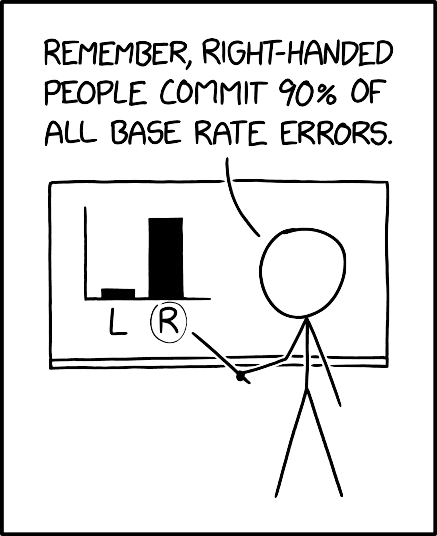
\includegraphics[width=0.3\textwidth]{imagenes/imagenes02/T03IM53.png}
	\end{figure}
\end{multicols}

\begin{flushright}
	 \textit{Martin Gardner. Selecciones del Reader’s Digest.}
\end{flushright}

\end{myexampleblock}


\vspace{5mm}	
\begin{myexampleblock} {El problema de probabilidad de los taxis de colores (y su curiosa solución)}


\vspace{2mm}Los problemas de probabilidad son divertidos y muy difíciles a veces, especialmente cuando el resultado de los cálculos desafía el sentido común. Los economistas Tversky y Kahneman crearon un problema de este tipo, realmente interesante, de esos que van contra la intuición. Más o menos viene a decir lo siguiente:

\vspace{2mm}\emph{``En una ciudad hay dos compañías de taxi: azules y verdes. Un 15\% de los taxis son azules y un 85\% son verdes. En un accidente nocturno, un testigo asegura que vió un taxi azul. Se sabe que gracias a unas pruebas independientes que ese testigo es capaz de identificar correctamente el color de un taxi el 80\% de las veces.\textbf{?`De color era el taxi?}’'}


\vspace{2mm}Casi todo el mundo que intenta resolver el problema cree que el taxi era seguramente azul. Pero el taxi era probablemente verde.

\vspace{2mm}Tal y como aprendimos en CSI lo fiable son los datos y las pruebas, no los testigos, que pueden confundir los colores de los coches, sobre todo en una noche oscura y bajo una luz amarilla.

\vspace{2mm}Ateniéndonos únicamente a los datos, como haría Grissom, el cálculo de probabilidades permite darse cuenta de que, en función de las cantidades de taxis y teniendo en cuenta la fiabilidad del testigo, la probabilidad de que el taxi fuera verde es del 59 por ciento, frente sólo a un 41 por ciento de que fuera azul.

\vspace{2mm}Lo que sucede es que la gente otorga subjetivamente un alto peso a la fiabilidad del 80\% del testigo, que es alta pero no perfecta. En cambio, la gran desproporción de taxis de un color y otro hace que algo improbable (que el taxi involucrado fuera azul, aun habiendo muchos menos taxis de ese color)siga siendo improbable, y que el testimonio carezca de valor.

\vspace{2mm}El calculo de estas probabilidades dista de ser trivial y se hace mediante una tabla o un árbol. 

\vspace{2mm}?`La moraleja? Que cuanto más improbable sea un hecho por su propia naturaleza, más carente de valor será la fiabilidad de un testigo que diga haberlo visto suceder, a menos que sea infalible.


\rule{50mm}{0.1mm}

\begin{flushright}
	\begin{footnotesize}
		De @ALVY, en \emph{microsiervos.com}, (20/02/2008)
	\end{footnotesize}
\end{flushright}

\rule{100mm}{0.1mm}

\begin{multicols}{2}
	\begin{figure}[H]
			\centering
			\includegraphics[width=0.5\textwidth]{imagenes/imagenes02/T02IM47.png}
	\end{figure}
	Puesto que el testigo asegura que el taxi accidentado es Azul, calculemos la probabilidad de que el taxi sea Azul/Verde, sabiendo que el testigo asegura que es Azul: $\ P(A|dice\ A)\ $ y $\ p(V|dice \ A)$:
	
	$\quad$ 
	
	\begin{small}$ P(A|dice\ A)=\dfrac{0.15\cdot 0.8}{0.15\cdot 0.8 + 0.85\cdot 0.2}=\boldsymbol{0.41}$\end{small}
	
	\begin{small}$ P(V|dice\ A)=\dfrac{0.85\cdot 0.2}{0.15\cdot 0.8 + 0.85\cdot 0.2}=\boldsymbol{0.59}$\end{small}
	
	$\quad$ 
	
	Es más probable (60\% frente 40\%, aprox.) que el taxi accidentado sea de color Verde.
	
\end{multicols}


	
\end{myexampleblock}


\vspace{5mm}
\begin{myexampleblock}
{La falacia del fiscal}

\begin{small}
``Señoría, tras hallar la sangre de la acusada en la escena del crimen todo queda más claro”, afirmaba el fiscal mientras sostenía su firme mirada ante la jueza. Poco después y tras un leve carraspeo, declaró: “no hay dudas de su culpabilidad''.\footnote{ http://anabelforte.com/2021/04/18/falacia-fiscal-probabilidad/}

\vspace{2mm} El fiscal, volvió a tomar asiento y repasó los papeles que tenia delante… la probabilidad de hallar el tipo de sangre de la acusada en la escena del crimen, siendo esta la culpable, era de casi un 98\%, y no llegaba al 100\% porque había una pequeña probabilidad de que la sangre no fuese de la persona que había cometido el crimen.

\vspace{2mm} Pero el fiscal se estaba equivocando en algo, estaba cometiendo la conocida \textbf{falacia del fiscal}. Pero ?`en qué se equivocaba? ?`En qué consiste esta falacia?

\vspace{2mm} ?`Me dejas que te cuente?

\vspace{2mm} \underline{Probabilidad Condicionada}


\vspace{2mm} Para poder entender en que se equivocaba el fiscal es importante que conozcamos un concepto básico, la probabilidad condicionada.

\vspace{2mm} Es fácil ser consciente de que determinados sucesos cambian el curso de los acontecimientos y, por tanto, la probabilidad de aquello que nos interesa.

\vspace{2mm} Empezando por un ejemplo muy sencillo, la probabilidad de que, al lanzar dos dados de 6 caras, la suma de los resultados sea 3 es de 2/36 (de las 36 posibles formas en las que caerán los dados, 2 de ellas tendrán una suma de 3 en los casos:  2+1 o 1+2). Sin embargo, si sabemos que en el primero de los dados nos ha salido un 1, la probabilidad aumenta a 1/6 porque ya solo depende de que en el segundo dado nos salga un 2. 

\vspace{2mm} Cuando estamos en este tipo de circunstancias hablamos de probabilidad condicionada y lo expresamos como la probabilidad de que suceda un evento A dado que ha sucedido cierto evento B o, en notación matemática P(A | B).

\vspace{2mm} Cabe mencionar que aquello a lo que condicionamos, lo que hemos llamado evento B, no siempre será algo que haya pasado antes si no que puede hacer referencia a determinadas circunstancias que hacen que cambié todo. Por ejemplo, la probabilidad de ingresar en UCI por la COVID-19 cambia según la franja de edad en la que te encuentras y, por tanto, estamos hablando de probabilidades condicionadas a tus circunstancias, no a algo que ya haya pasado.  

\vspace{2mm} Una cuestión importante cuando hablamos de probabilidad condicionada es entender que se trata, al fin y al cabo, de una probabilidad para el evento A. ¿Y qué quiero decir con esto?, pues que nos estamos centrando en la probabilidad del evento A, aunque sea bajo unas condiciones concretas B. Y aquí, el orden de los factores sí altera el resultado, es decir, la probabilidad de que pase A dadas las condiciones B no serán nunca las mismas que la probabilidad del evento B bajo las condiciones A.  

\vspace{2mm} A este error es a lo que llamamos en probabilidad la \emph{`falacia del fiscal’} y es un error de interpretación mucho más común de lo que pensamos. 

\vspace{2mm} \underline{Una falacia común}

\vspace{2mm} Volviendo al ejemplo de los dos dados, hemos visto que la probabilidad de que sumen 3 bajo la condición de que el primero de ellos había dado 1 era de 1/6. Pero, si condicionamos a que la suma sea 3, sabemos que el primer dado solo ha podido dar como resultado 1 o 2, por tanto, la probabilidad de que haya salido un 1 en esas circunstancias sería de 1/2, muy distinta de la primera.

\vspace{2mm} Puede parecer obvio en este ejemplo pero, la cuestión es que, confundir estas probabilidades es un error típico, por ejemplo, en la detección de enfermedades. 

\vspace{2mm} \underline{Después de un positivo}

\vspace{2mm} Imaginad que os hacen una prueba para ver si sufrís una determinada enfermedad. Toda prueba de este tipo tiene asociada una probabilidad de dar positivo bajo la condición de sufrir realmente la enfermedad. Este valor, conocido como \textbf{sensibilidad}, suele ser bastante alto. Pongamos que en nuestro ejemplo es de 98\%. También tiene una probabilidad de dar negativo cuando no se tiene la enfermedad. Este valor es conocido como \textbf{especificidad} y también suele ser alta. Pongamos que es de un 95\% en este caso

\vspace{2mm} Ante estas condiciones, obtener un positivo puede suponer un drama. Puede parecer que la probabilidad de tener la enfermedad es del 0.98, pero… recapitulemos. 

\vspace{2mm} En este caso, el evento de interés (A) es “tener la enfermedad” y lo que ya es conocido (B) es “haber dado positivo”. Buscamos entonces la probabilidad P(tener la enfermedad|haber dado positivo).


\vspace{2mm} Sin embargo, la sensibilidad hace referencia a la probabilidad de dar positivo dado que se tiene la enfermedad, esto es: P(haber dado positivo | tener la enfermedad) = 0.98 y, como ya hemos visto, no tiene porque ser la misma que la anterior.

\vspace{2mm} Pero seguro que ahora os ha surgido una pregunta ?`podemos calcular la primera en función de la segunda?

\vspace{2mm} Esto es lo que se denomina el problema de la probabilidad inversa y la respuesta es sí. De hecho, aquí aparece uno de los teoremas que más me gustan y que, como ya sabéis, es el teorema de Bayes.



\vspace{2mm} \underline{A vueltas con el teorema de Bayes}



\vspace{2mm} En el Teorema de Bayes que aparecen dos elementos además de las probabilidades condicionadas. El primero es P(A) que, en el caso de la enfermedad representa la probabilidad de sufrirla (con positivo o sin positivo). Este valor recibe el nombre de \textbf{incidencia de la enfermedad} y si estamos hablando de una enfermedad rara, será muy bajita, pongamos de 0.001. Por otra parte, P(B) es la probabilidad de que la prueba sea positiva, sin importar si se está enfermo o no. Esta probabilidad, si bien no la sabemos directamente, se puede calcular como:

\vspace{2mm} P(positivo | enfermedad) $\cdot$ P(enfermedad) + P(positivo | No enfermedad) $\cdot$ P(No enfermedad)  \textcolor{gris}{ (este es el conocido \emph{Teorema de la Probabilitdad Total})}.

\vspace{2mm} Pues bien, vayamos a los números:

\vspace{2mm} --- P(enfermedad) = 0.001, 

--- P(No enfermedad) = 0.999; 

--- P(positivos | enfermedad) =0.98, la \emph{`sensibilidad’}; 

--- P(positivo | No enfermedad) = 1- \emph{`especificidad’} = 1-0.95 = 0.05 

\vspace{2mm} Usando entonces el teorema de Bayes, se llega a una probabilidad de sufrir la enfermedad habiendo obtenido un positivo de 0.02. Un valor muy bajo que no tiene nada que ver con la seguridad que en un inicio nos alarmó.

\vspace{2mm} Pues bien, ahora que hemos entendido que es esto de la probabilidad condicionada y la probabilidad inversa, es hora de volver con nuestro fiscal.

\vspace{2mm} \underline{Volviendo al juicio}

\vspace{2mm} La probabilidad que nuestro fiscal venía manejando era la de haber hallado ese tipo de sangre si la acusada era realmente culpable. Sin embargo, la que le debía interesar realmente, era la de que la acusada fuera culpable dada la única prueba disponible: una muestra de sangre tipo $0-$.


\vspace{2mm} Hemos visto que, usando el Teorema de Bayes como en el caso de la enfermedad, el fiscal podía dar la vuelta a la probabilidad que sí que tenía: P(tipo de sangre $0-$ en la escena del crimen | la acusada cometió el crimen)=0.98 para convertirla en la que realmente le interesaba. Solo necesitaba un valor inicial para la probabilidad de culpabilidad, P(A).



\vspace{2mm} \underline{Juguemos  con los números}



\vspace{2mm} Supongamos que empezamos por creer que la acusada es inocente y damos una probabilidad muy baja a su culpabilidad, de 0.01, por ejemplo. Ahora solo nos falta el denominador, P(B), que en este caso es P(tipo de sangre $0-$ en la escena del crimen). Utilizando de nuevo el teorema de la probabilidad total, podemos calcularla como:

\vspace{2mm} P(tipo $0-$ | la acusada es culpable) $\cdot$ P(culpable) + P(tipo $0-$ | no culpable) $\cdot$ P(no culpable)

\vspace{2mm} Ya sabemos que la primera probabilidad que aparece es la que manejaba el fiscal y tiene un valor de 0.98, la segunda es la de culpable que hemos prefijado en 0.01. Después tenemos la probabilidad de haber hallado ese tipo de sangre si no tenemos ni idea de quien cometió el crimen. Asumimos que esa probabilidad es la misma que en la población general, que para el grupo $0-$ es de 0.07. Por último, tenemos la probabilidad de nos ser culpable que será 1-0.01=0.99.

\vspace{2mm} Combinando todos estos valores y utilizando el Teorema de Bayes nos queda que la probabilidad de que la acusada sea culpable es de 0.12, mucho menor que la probabilidad que manejaba el fiscal. Cabe destacar que, cuanto mas raro sea el tipo de sangre, es decir, más especifica sea la prueba, mayor será la probabilidad de que sea culpable.


\vspace{2mm} \underline{No solo un ejemplo}

\vspace{2mm} El error que cometía nuestro fiscal y que ya hemos dicho que se conoce como la \emph{falacia del fiscal o Prosecutor’s Fallacy}, en inglés, no es solo un ejemplo de juguete. Uno de los casos más famosos en los que esta falacia llevó a la cárcel, injustamente, a una persona, fue en el juicio contra Sally Clark. Sally estaba acusada de haber asesinado a sus dos hijos pequeños. Los dos pequeños de la familia Clark habían sufrido muerte súbita, un suceso muy triste pero que se produce de forma natural en los primeros meses de vida de algunos bebés.



\vspace{2mm} Durante el juicio, se incurrió en la falacia del fiscal al considerar lo probable que era que los niños hubiesen muerto si la madre había sido la culpable, pero no la probabilidad de culpabilidad de la madre que se veía considerablemente reducida si se consideraban todas las posibles causas de muerte y, sobre todo, que la muerte súbita podía tener que ver con la genética de los bebes y, por tanto, ser más común entre hermanos.



\vspace{2mm} Así pues, solo me queda decir que no os dejéis llevar por las apariencias, y que siempre penséis con claridad en cual es el evento del que queréis calcular su probabilidad, no vayamos a darle la vuelta.


\vspace{2mm} !Gracias por leer hasta aquí!

\rule{50mm}{0.1mm}

Artículo del blog de Anabel Forte \emph{(anabelforte.com)}, doctora en Matemáticas y en Ciencias y Técnicas Estadísticas por la Universitat de València. 

\end{small}
	
\end{myexampleblock}



%\newpage
%\includepdf[pages=-]{imagenes/imagenes02/resumen-probabilidad.pdf}

\newpage

$\quad$

$\quad$

\begin{myblock}{RESUMEN: Cálculo de probabilidades}
$\quad$



\vspace{5mm} $\triangleright \ $ Definiciones a posteriori y a priori de probabilidad:

$$p(A)=\lim_{N\to \infty} \dfrac{N_A}{N} \ \ \text{ Ley grandes números} \ ;
\quad \quad
p(A)=\dfrac{\text{favorables}}{\text{posibles}} \ \ \text{ Ley de Laplace}$$

\vspace{5mm} $\triangleright \ $ Axiomática de Kolmogorov:

$$p(\varPhi)=0 \le \ p(A)\ \le 1=p(E)\ ; \qquad
p(A')=1-p(A) \ ; \qquad
p(A\cup B)=p(A)+p(B)-p(A\cap B)  $$

\vspace{5mm} $\triangleright \ $ Probabilidad condicionada:

$$p(A|B)=\dfrac{p(A\cap B)}{p(B)} \ ;
\qquad \qquad 
\left\{ \ 
\begin{matrix}
	A, B \text{ independientes si } p(A|B)=p(A) 
	\\
	A, B \text{ incompatibles si } p(A\cap B)=\varPhi \ \ \ \ 
\end{matrix} \right.$$

$$ A \text{ y } B \text{ independiente } \leftrightarrow p(A\cap B)=p(A) \cdot p(B)$$
 

\vspace{5mm} $\triangleright \ $ Teoremas de la probabilidad total y de Bayes:

	\begin{figure}[H]
			\centering
			\includegraphics[width=.6\textwidth]{imagenes/imagenes02/T02IM22.png}
	\end{figure}

$\quad p(S)=p(S|A_1)\cdot p(A_1) \cdot p(S|A_2)\cdot p(A_2) \cdot \cdots 	\cdot p(S|A_n)\cdot p(A_n) $

$\quad$

$\quad p(A_i|B= \ = \ \dfrac{p(A_i) \cdot p(S|A_i)}{p(S)}$

$\quad$
\end{myblock}



